\chapter{Aplicação a dados sintéticos}

\section{Modelo simples}

Foi simulado um corpo geológico simples imerso em meio não magnético (prismas azuis nas Figuras 
\ref{fig:simple_model}, \ref{fig:simple_l2_result} e \ref{fig:simple_l1_result})
que representa a fonte alvo 3D com profundidade do topo em $0$ m, profundidade da base em $1600$ m, centro em $ (x_0, y_0) = (0, 0) $ e um vetor de magnetização total constante com inclinação $-50^{\circ}$, declinação $9^{\circ}$, e intensidade $9$ A/m.
Esse modelo é composto de $ 8 $ prismas com $ 20 $ vértices cada e raios que diminuem com a profundidade: ($ 1920 $ m, $ 1760 $ m, $ 1600 $ m, $ 144 $ m, $ 1280 $ m, $ 1120 $ m, $ 960 $ m, $ 800 $ m).
Recuperar a geometria desse corpo é uma tarefa relativamente simples para este método porque ele possui um alinhamento vertical e suas fatias horizontais mostram uma forma circular que diminui de tamanho ao longo da profundidade, assim, é possível notar que o corpo satisfaz perfeitamente quase todos os vínculos impostos neste método.
A anomalia de campo total (Figura \ref{fig:simple_model}a) produzida pela fonte alvo foi calculada em $1939$ pontos localizados sobre uma malha irregular com linhas que simulam um levantamento aéreo (Figura \ref{fig:simple_model}b) no plano $ z=-150 $ m. Esses dados sintéticos foram contaminados com um ruído Gaussiano pseudo-aleatório de média zero e desvio padrão igual a $5$ nT.
O método foi aplicado para inverter esse dado contaminado com ruído e obter soluções L2 e L1.
Para cada tipo de solução, foram geradas $36$ soluções L2 e $36$ soluções L1, 
todas elas foram obtidas com a mesma malha de varredura $6 \times 6$ de profundidades do topo $z_{0}$ e intensidade de magnetização total $m_{0}$.
A melhor solução L2 e L1 são definidas como aquelas que produzem o menor valor da função objetivo para cada caso.

A Figura \ref{fig:simple_model_rtp} mostra a anomalia RTP obtida via camada equivalente a partir da anomalia de campo total contaminada com ruído (Figura \ref{fig:simple_model}a) e 
a projeção horizontal das aproximações iniciais $\hat{\mathbf{p}}_{(0)}$ 
usadas nas sucessivas inversões (Figuras \ref{fig:simple_l2_result} e 
\ref{fig:simple_l1_result}).
As aproximações iniciais são compostas de $ L= 5$ prismas com $ V = 20 $ vértices, mesma direção de magnetização do corpo verdadeiro, espessura $ dz=350 $ m e centro em $ (x_0, y_0) = (0, 0) $.
A Figura \ref{fig:simple_l2_result}a mostra que a melhor solução L2 foi obtida através dos valores verdadeiros da profundidade do topo $z_{0}$ e intensidade de magnetização total $m_{0}$. Essa solução L2 produz um ótimo ajuste dos dados (Figura \ref{fig:simple_l2_result}b), possui uma profundidade da base em $1531.1$ m e também recupera a geometria do corpo verdadeiro (Figura \ref{fig:simple_l2_result}d).
A Figura \ref{fig:simple_l1_result} mostra um resultado similar, porém com um ajuste dos dados e geometria inferiores aos da solução L2. A profundidade da base foi estimada em $1756.9$ m.
Podemos observar que nesse teste ambas as abordagens L2 e L1 foram bem sucedidas em estimar a forma do corpo e recuperam as feições principais da fonte alvo. Entretanto, nesse caso, a solução L2 foi ligeiramente superior à solução L1.
Todas as soluções L2 e L1 produzidas neste teste foram obtidas usando o seguinte conjunto de pesos normalizados $\tilde{\alpha}_{\ell}$ (Equação \ref{eq:alphas}): 
$\tilde{\alpha}_{1} = 10^{-4}$, $\tilde{\alpha}_{2} = 10^{-5}$, 
$\tilde{\alpha}_{3} = 10^{-4}$, $\tilde{\alpha}_{4} = 10^{-8}$, e 
$\tilde{\alpha}_{5} = 10^{-4}$. 
É importante notar que, mesmo a solução L2 sendo superior à L1, não há diferenças significativas entre as soluções L2 e L1 obtidas pelo método.

\begin{figure}[!htb]
	\centering
	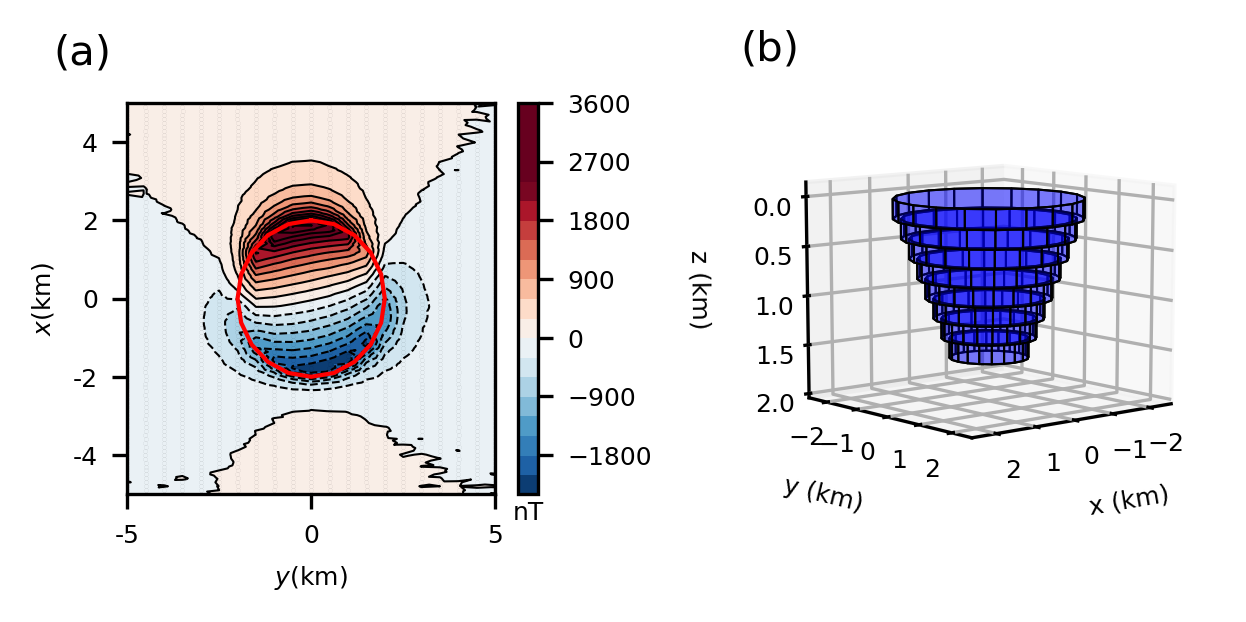
\includegraphics[width=\textwidth]{simple_model_data.png}
	\caption{Modelo simples. (a) Anomalia de campo total contaminada com ruído produzida pela fonte simples (prismas azuis mostrados nos painel b). Os pontos pretos representam os pontos de observação. O círculo vermelho representa a projeção horizontal da aproximação inicial $\hat{\mathbf{p}}_{(0)}$ (prismas vermelhos nas Figuras
		\ref{fig:simple_l2_result}c). %e \ref{fig:simple_l1_result}c). 
		(b) Visualização em perspectiva do modelo da fonte simples representada pelos prismas azuis.
	}
	\label{fig:simple_model}
\end{figure}

\pagebreak

\begin{figure}[!htb]
	\centering
	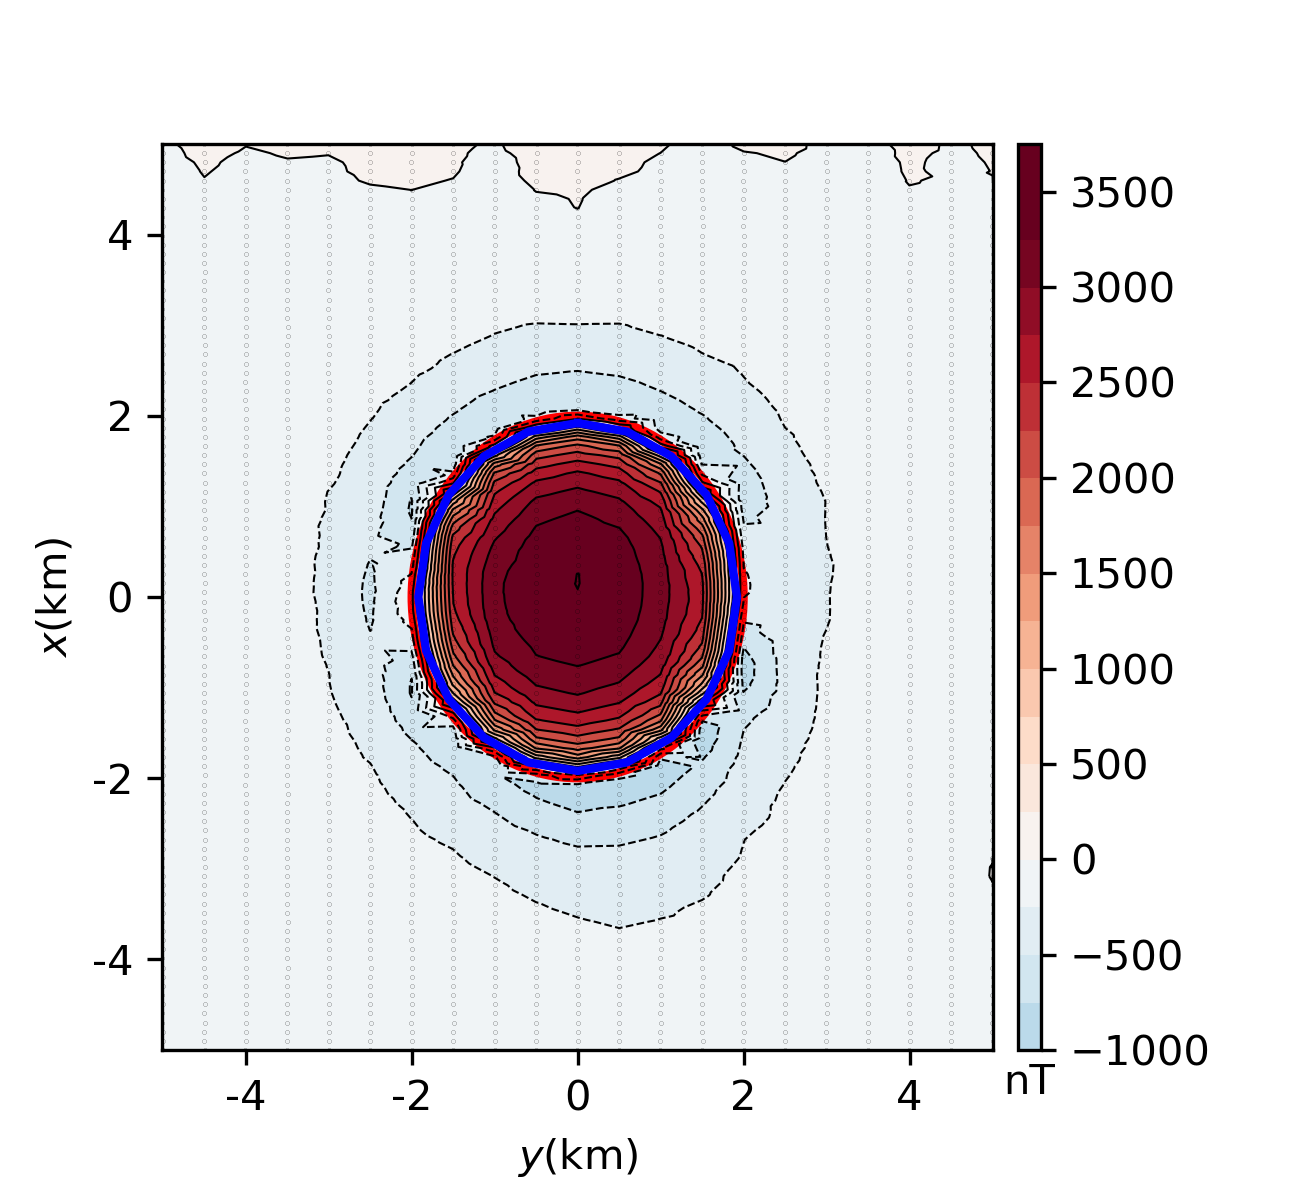
\includegraphics[width=\textwidth]{simple_rtp.png}
	\caption{Anomalia RTP produzida pela fonte simples. 
		A anomalia RTP mostra valores predominantemente positivos logo acima da fonte simples. Os pontos pretos representam os pontos de observação. As linhas azuis e vermelhas correspondem, respectivamente, às projeções horizontais da porção mais rasa da fonte alvo e da aproximação inicial utilizada nas inversões subsequentes (prismas vermelhos nas Figuras \ref{fig:simple_l2_result}c e 
		\ref{fig:simple_l1_result}c).
	}
	\label{fig:simple_model_rtp}
\end{figure}

\pagebreak

\begin{figure}[!htb]
	\centering
	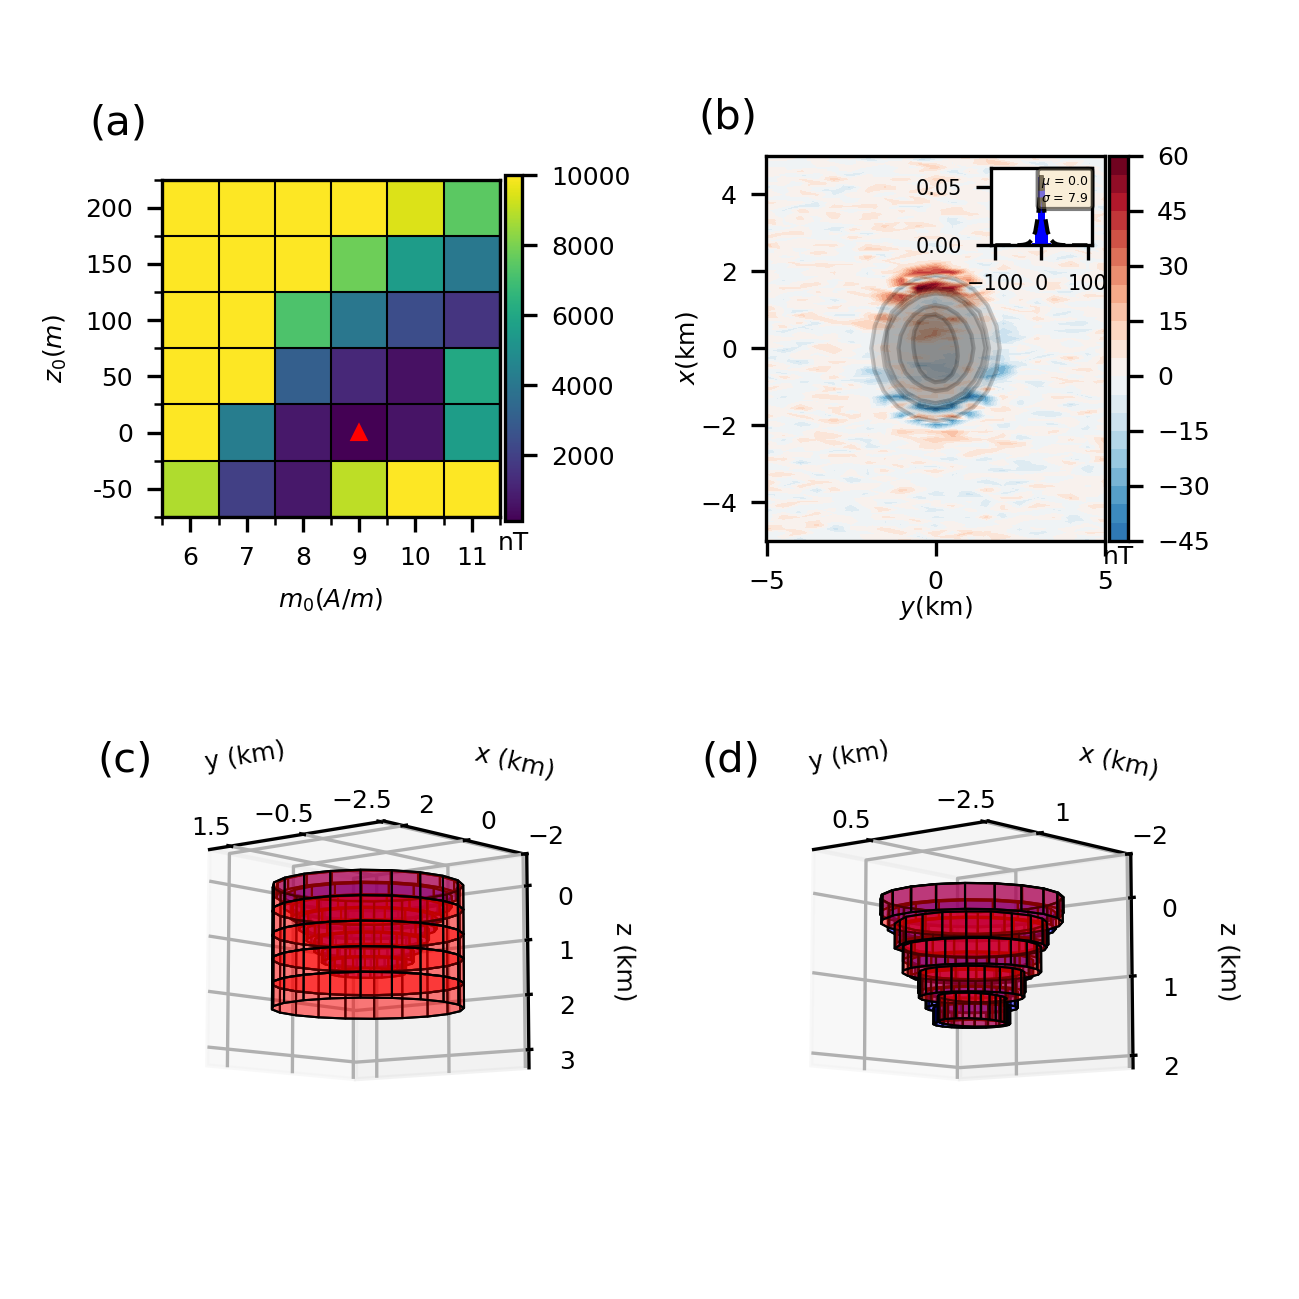
\includegraphics[width=\textwidth]{simple-l2-solution.png}
	\caption{Soluções L2 obtidas para o modelo da fonte simples. 
		(a) Mapa discreto da função objetivo produzida pelos modelos obtidos a partir da varredura de valores de profundidade do topo $z_{0}$ e intensidade de magnetização total $m_{0}$. 
		O triângulo vermelho representa os valores verdadeiros para $m_{0}$ e $z_{0}$, assim como os valores que definem a melhor solução L2.
		(b) Resíduos entre os dados contaminados com ruído (Figura \ref{fig:simple_model}a) 
		e os dados preditos (não mostrados) produzidos pela melhor solução L2 (prismas vermelhos no painel d). 
		O histograma dos resíduos inserido em (b) mostra a curva Gaussiana ajustada (linha tracejada).
		Os polígonos cinzas representam as projeções horizontais de todos os prismas que compõe a melhor solução. 
		(c) e (d) Visualização em perspectiva da aproximação inicial (prismas vermelhos) e 
		a melhor solução (prismas vermelhos), respectivamente. Os prismas azuis são o modelo da fonte simples. 
	}
	\label{fig:simple_l2_result}
\end{figure}
\pagebreak

\begin{figure}[!htb]
	\centering
	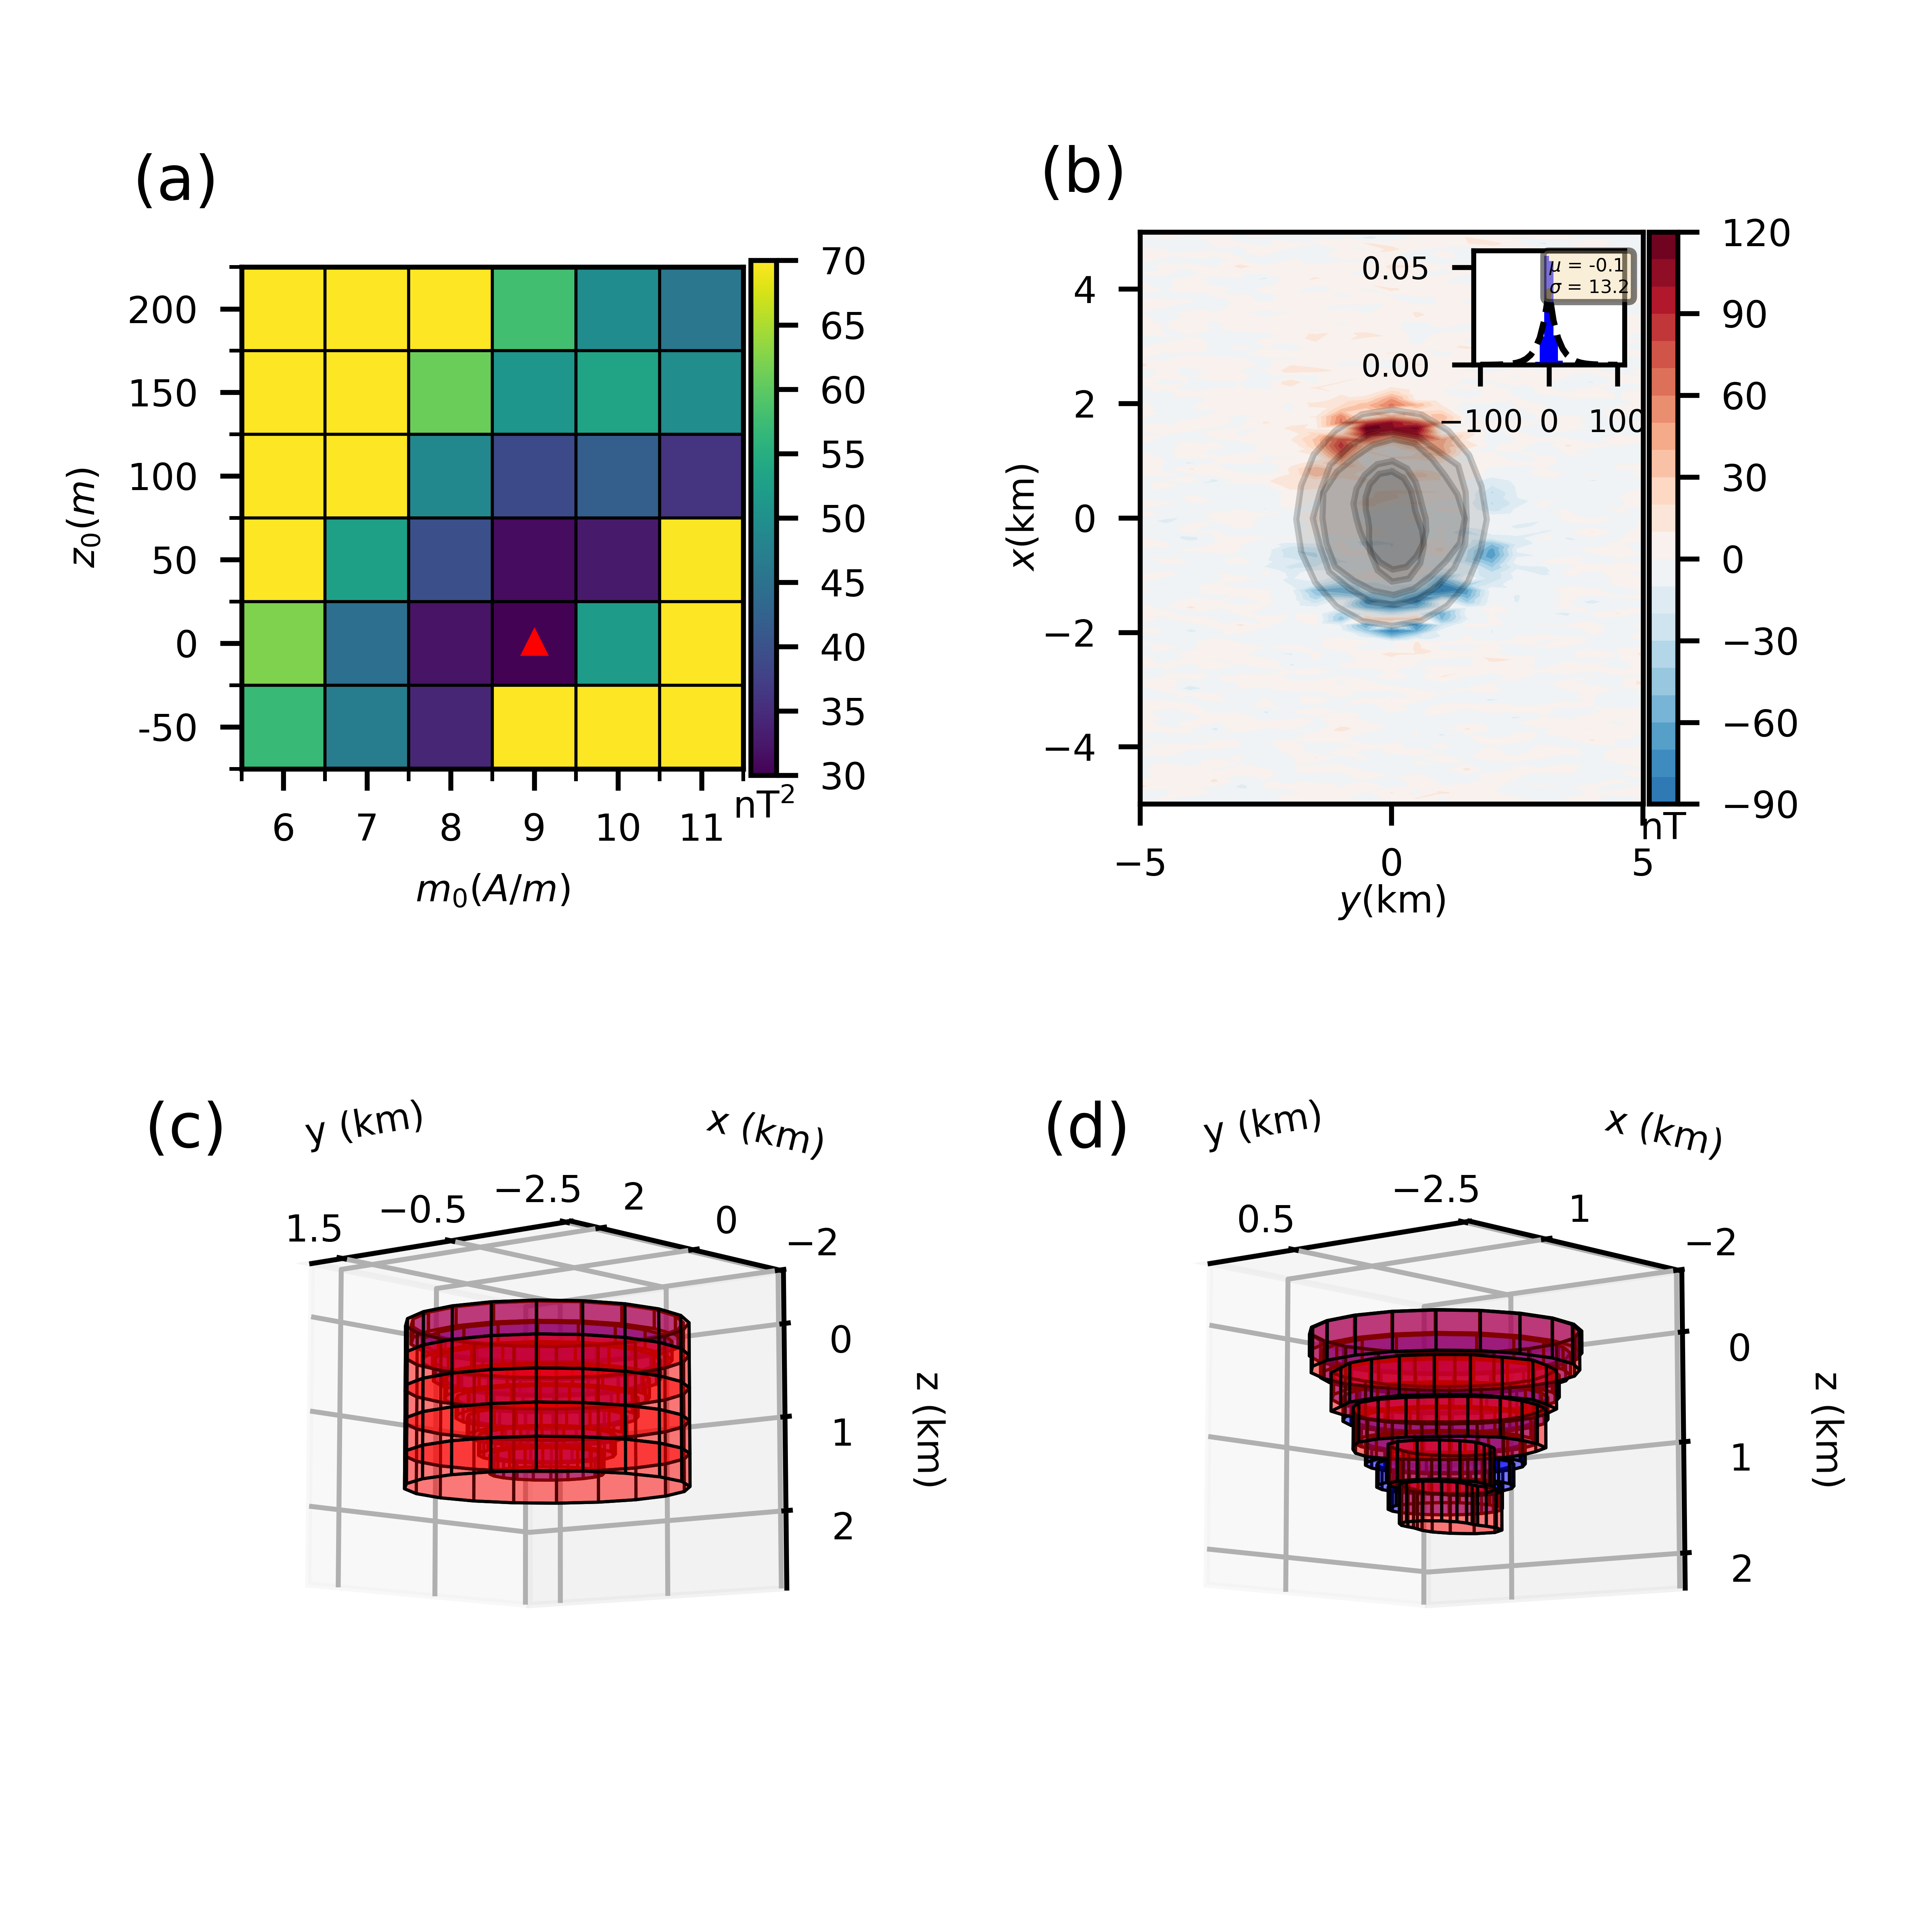
\includegraphics[width=\textwidth]{simple-l1-solution.png}
	\caption{Soluções L1 obtidas para o modelo da fonte simples. 
		(a) Mapa discreto da função objetivo produzida pelos modelos da malha de varredura para valores de profundidade do topo $z_{0}$ e intensidade de magnetização total $m_{0}$. 
		O triângulo vermelho representa os valores verdadeiros para $m_{0}$ e $z_{0}$, assim como os valores que definem a melhor solução L1.
		(b) Resíduos entre os dados contaminados com ruído (Figura \ref{fig:simple_model}a) 
		e os dados preditos (não mostrados) produzidos pela melhor solução L1 (prismas vermelhos no painel d). 
		O histograma dos resíduos inserido em (b) mostra a curva Laplaciana ajustada (linha tracejada).
		Os polígonos cinzas representam as projeções horizontais de todos os prismas que compõe a melhor solução. 
		(c) e (d) Visualização em perspectiva da aproximação inicial (prismas vermelhos) e 
		a melhor solução (prismas vermelhos), respectivamente. Os prismas azuis são o modelo da fonte simples. 
	}
	\label{fig:simple_l1_result}
\end{figure}

\pagebreak

\section{Modelo inclinado}

Para verificar se o método é capaz de recuperar um corpo que possui um mergulho pouco acentuado, foi simulado um corpo geológico inclinado imerso em meio não magnético (prismas azuis nas Figuras 
\ref{fig:inclined_model}, \ref{fig:inclined_l2_result} e \ref{fig:inclined_l1_result})
que representa a fonte alvo 3D com profundidade do topo em $0$ m, profundidade da base em $3040$ m, centro em $ (x_0, y_0) = (-300, 600) $ e um vetor de magnetização total constante com inclinação $-50^{\circ}$, declinação $9^{\circ}$, e intensidade $9$ A/m.
Esse modelo é composto de $ 8 $ prismas com $ 20 $ vértices.
Recuperar a geometria desse corpo simulado é uma tarefa relativamente complicada para este método porque ele possui um mergulho acentuado em uma direção aproximadamente N-S e suas fatias horizontais mostram uma forma irregular que varia de tamanho ao longo da profundidade, assim, é possível notar que o corpo não satisfaz os vínculos impostos neste método.
A anomalia de campo total (Figura \ref{fig:inclined_model}a) produzida pela fonte alvo foi calculada em $1674$ pontos localizados sobre uma malha irregular com linhas que simulam um levantamento aéreo (Figura \ref{fig:inclined_model}b). Esses dados sintéticos foram contaminados com um ruído Gaussiano pseudo-aleatório de média zero e desvio padrão igual a $5$ nT.
O método foi aplicado para inverter esse dado contaminado com ruído e obter soluções L2 e L1.
Para cada tipo de solução, foram geradas $36$ soluções L2 e $36$ soluções L1, 
todas elas foram obtidas com a mesma malha de varredura $6 \times 6$ de profundidades do topo $z_{0}$ e intensidade de magnetização total $m_{0}$.
A melhor solução L2 e L1 são definidas como aquelas que produzem o menor valor da função objetivo para cada caso.

A Figura \ref{fig:inclined_model_rtp} mostra a anomalia RTP obtida a partir da anomalia de campo total contaminada com ruído (Figura \ref{fig:inclined_model}a) e 
a projeção horizontal das aproximações iniciais $\hat{\mathbf{p}}_{(0)}$ 
usadas nas sucessivas inversões (Figuras \ref{fig:inclined_l2_result} e 
\ref{fig:inclined_l1_result}).
As aproximações iniciais são compostas de $ L= 5$ prismas com $ V = 20 $ vértices, mesma direção de magnetização do corpo verdadeiro, espessura $ dz=350 $ m e centro em $ (x_0, y_0) = (-200, 0) $.
A Figura \ref{fig:inclined_l2_result}a mostra que a melhor solução L2 obtida superestima a profundidade do topo $z_{0}$ e acerta o valor da intensidade de magnetização total $m_{0}$ verdadeira. Essa solução L2 produz um ótimo ajuste dos dados (Figura \ref{fig:inclined_l2_result}b), possui uma profundidade da base em $3453.0$ m e também recupera a geometria do corpo verdadeiro (Figura \ref{fig:inclined_l2_result}d).
A Figura \ref{fig:inclined_l1_result} mostra um resultado similar, porém a profundidade da base estimada em $3107.2$ m foi muito próxima da verdadeira.
Podemos observar que nesse teste ambas as abordagens L2 e L1 foram bem sucedidas em estimar a forma do corpo e recuperam as feições principais da fonte alvo. Entretanto, nesse caso, a solução L1 foi ligeiramente superior à solução L2.
Todas as soluções L2 produzidas neste teste foram obtidas usando o seguinte conjunto de pesos normalizados $\tilde{\alpha}_{\ell}$ (Equação \ref{eq:alphas}): 
$\tilde{\alpha}_{1} = 10^{-3}$, $\tilde{\alpha}_{2} = 10^{-3}$, 
$\tilde{\alpha}_{3} = 10^{-6}$, $\tilde{\alpha}_{4} = 10^{-6}$, e 
$\tilde{\alpha}_{5} = 10^{-5}$. 
Já as soluções L1 foram obtidas utilizando o conjunto: 
$\tilde{\alpha}_{1} = 10^{-4}$, $\tilde{\alpha}_{2} = 10^{-4}$, 
$\tilde{\alpha}_{3} = 10^{-6}$, $\tilde{\alpha}_{4} = 10^{-6}$, e 
$\tilde{\alpha}_{5} = 10^{-5}$.
É importante notar que, mesmo a solução L1 sendo superior à L2, não há diferenças significativas entre as soluções L2 e L1 obtidas pelo método.


\begin{figure}[!htb]
	\centering
 	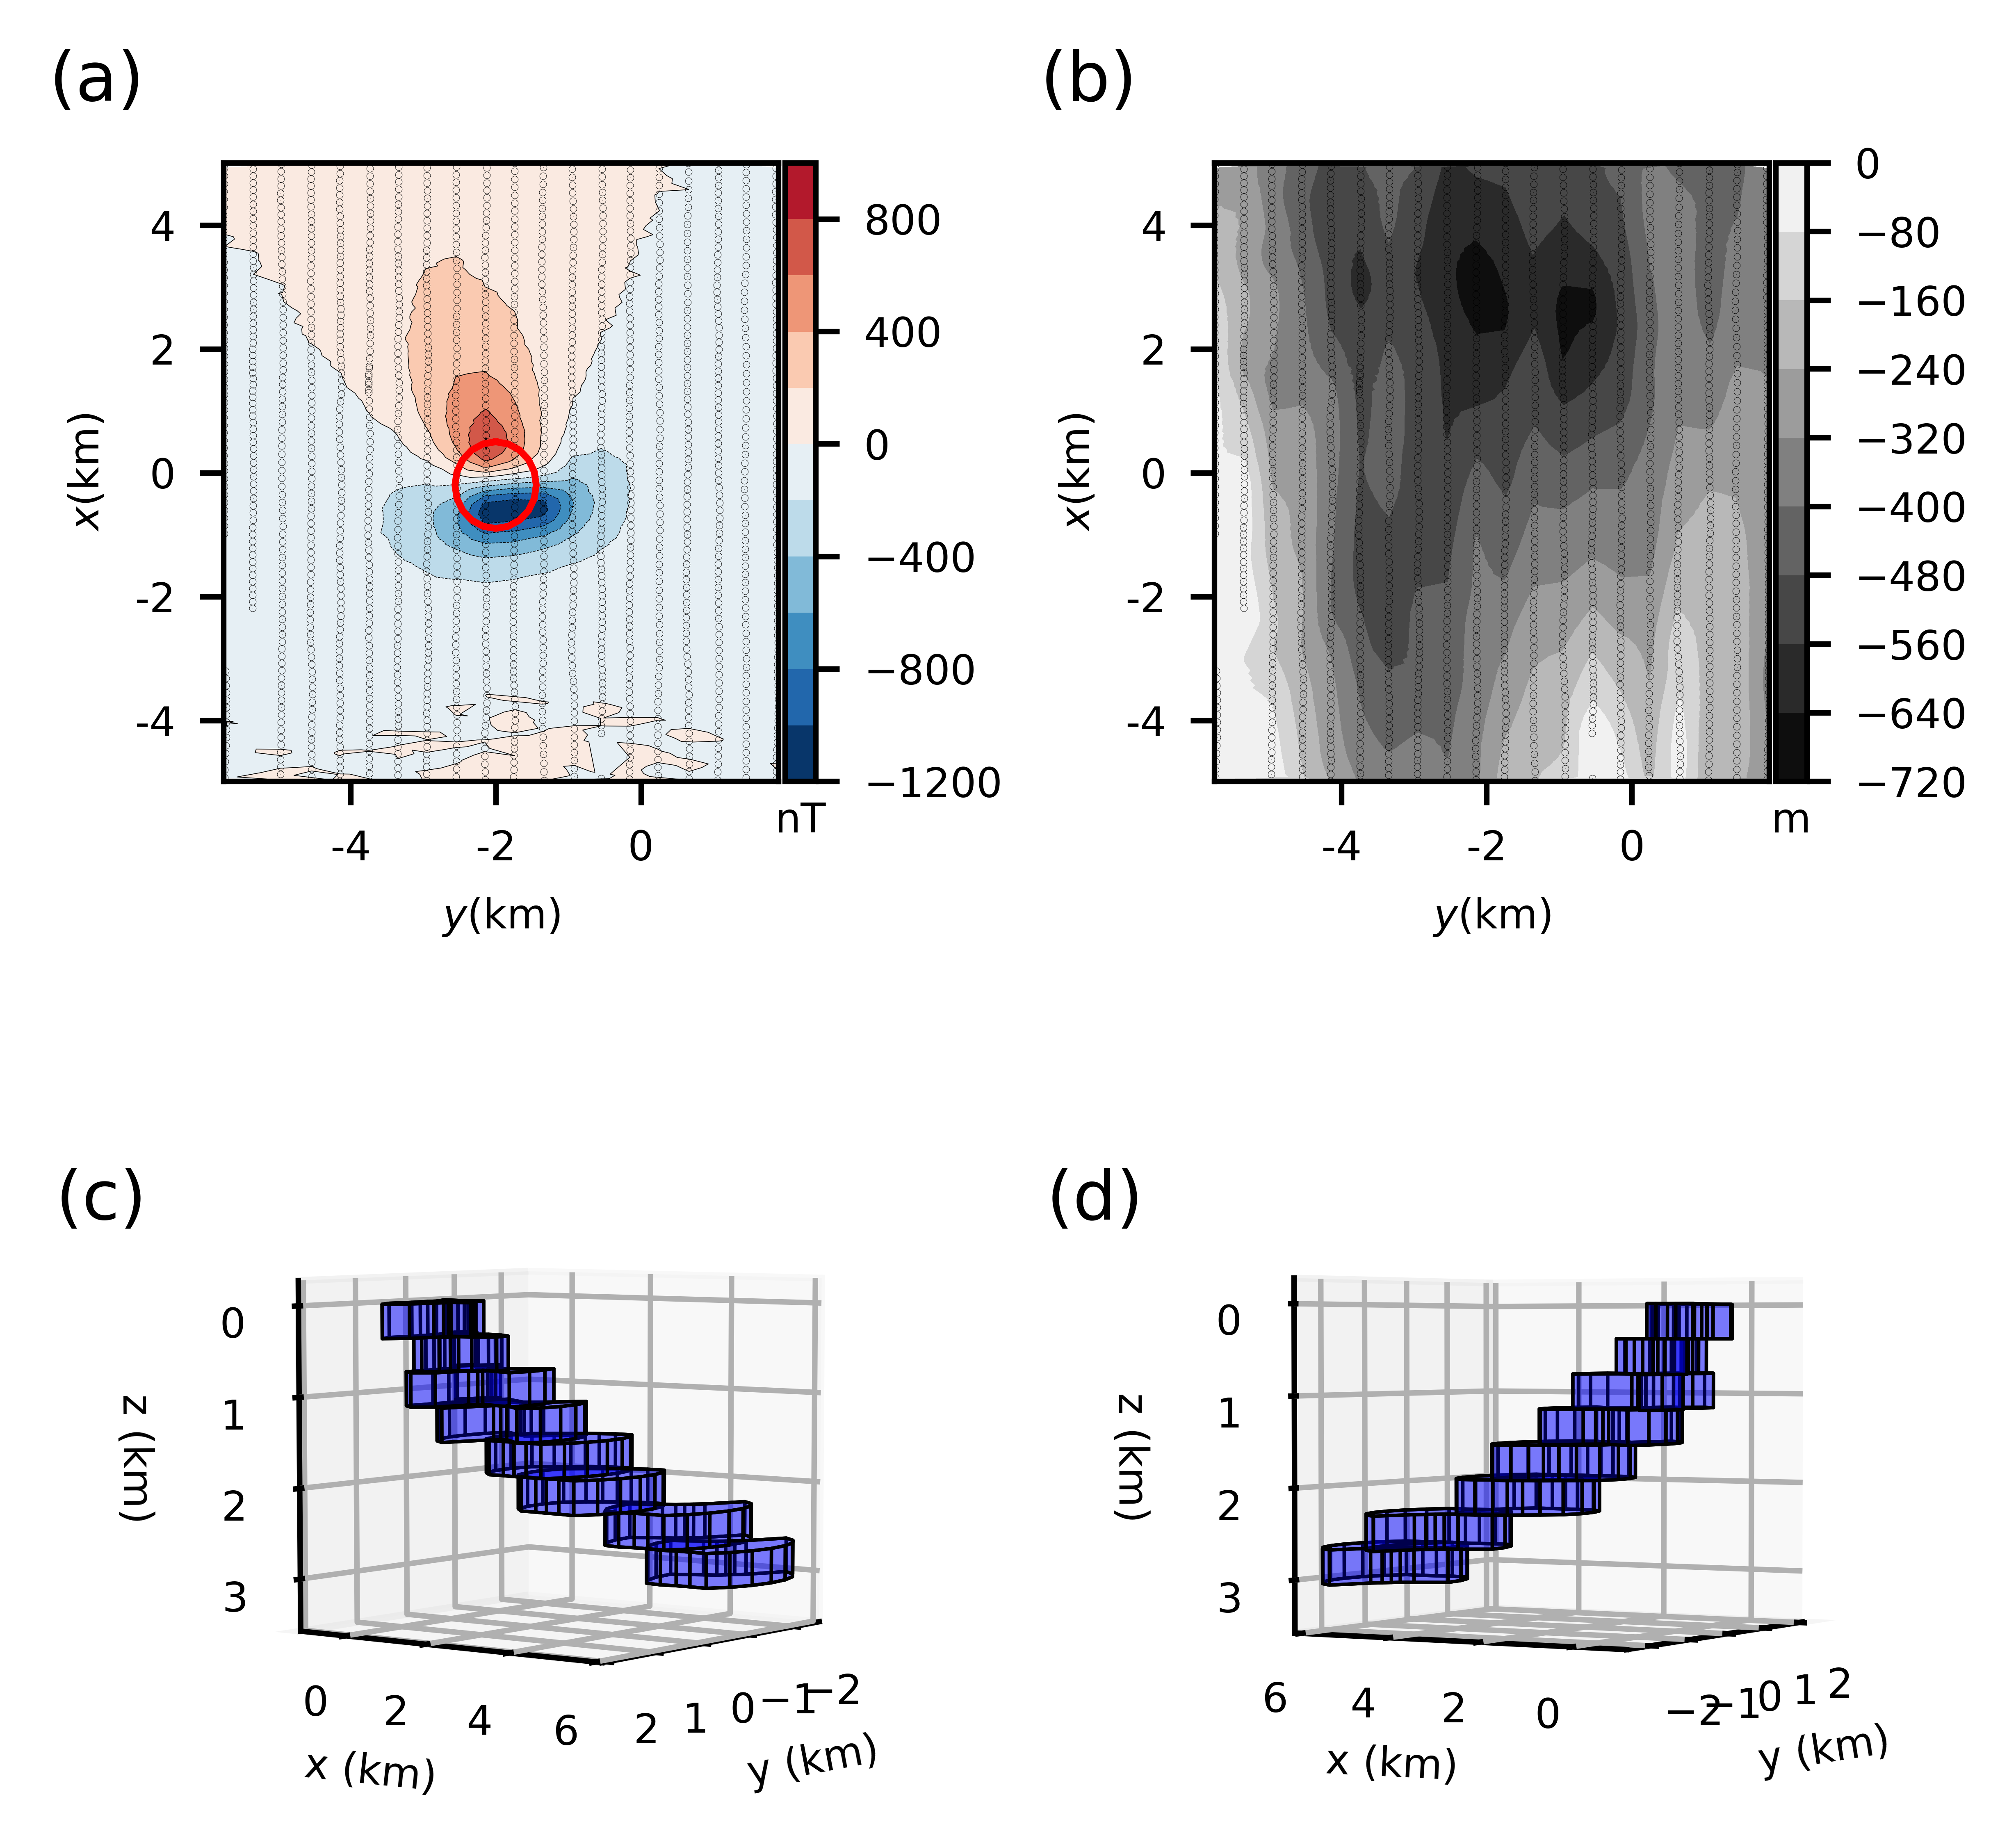
\includegraphics[width=\textwidth]{inclined_model_data.png}
	\caption{Modelo inclinado. (a) Anomalia de campo total contaminada com ruído produzida pela fonte alvo (prismas azuis mostrados nos painéis c e d). Os pontos pretos representam os pontos de observação. O círculo vermelho representa a projeção horizontal da aproximação inicial $\hat{\mathbf{p}}_{(0)}$ (prismas vermelhos nas Figuras
		\ref{fig:inclined_l2_result}c e \ref{fig:inclined_l1_result}c). (b) Coordenadas verticais dos pontos de observação que simulam um levantamento aéreo.
		(c) e (d) Visualizações em perspectiva do modelo da fonte alvo representada pelos prismas azuis.
	}
	\label{fig:inclined_model}
\end{figure}
\pagebreak

\begin{figure}[!htb]
	\centering
	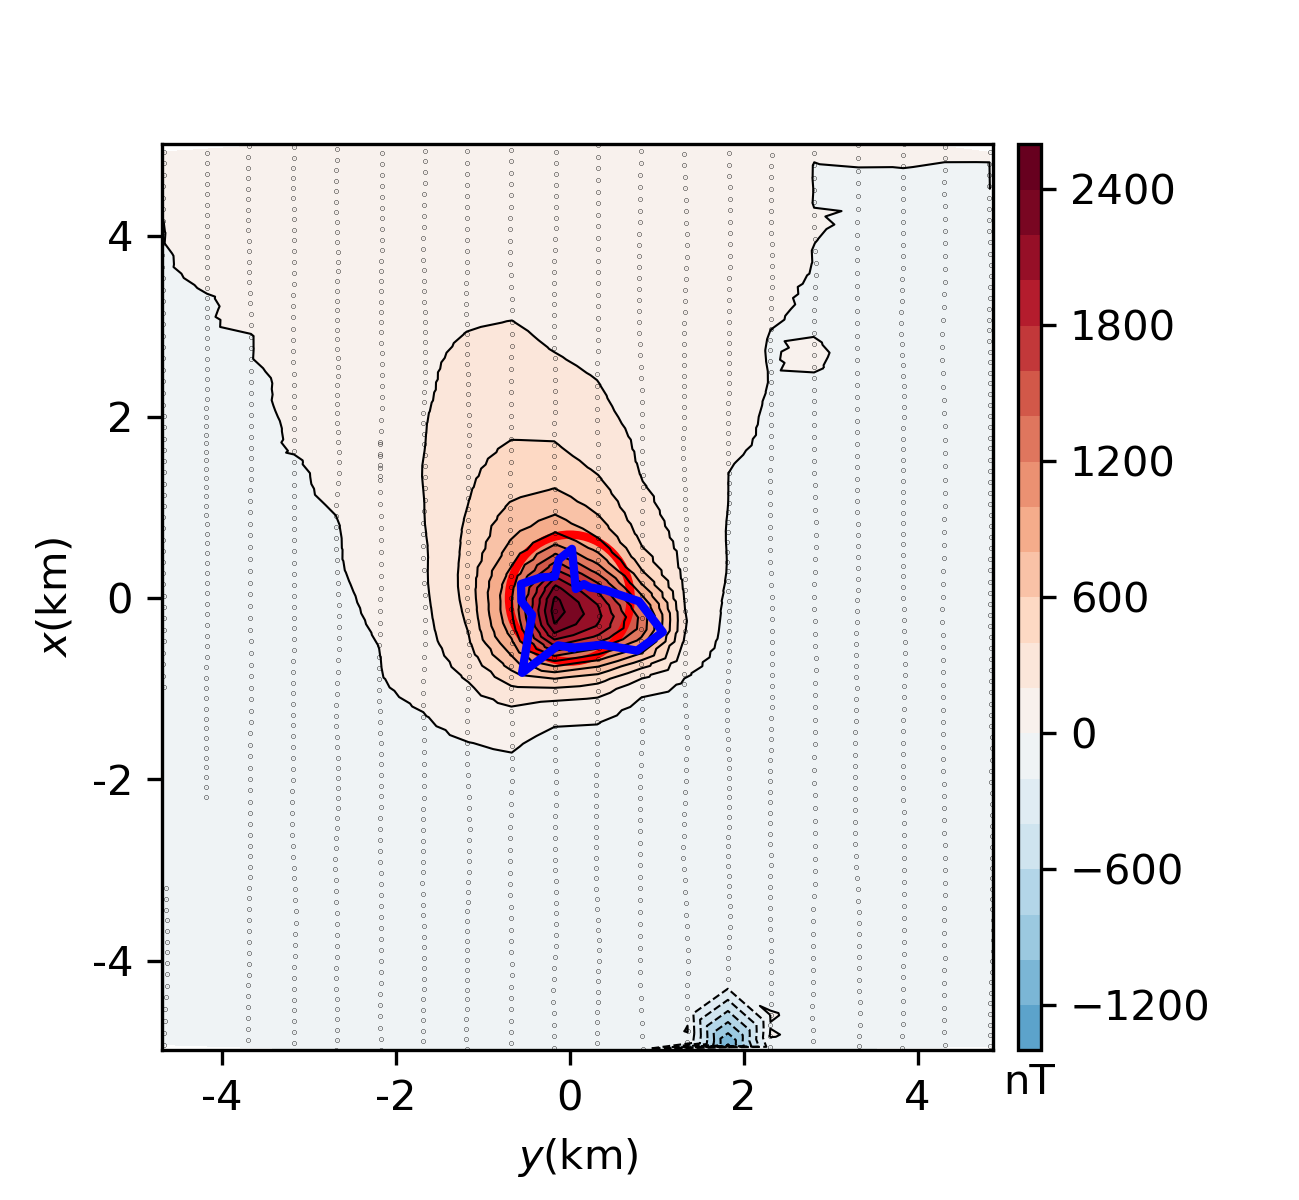
\includegraphics[width=\textwidth]{inclined_rtp.png}
	\caption{Anomalia RTP produzida pela fonte alvo. 
		A anomalia RTP mostra valores predominantemente positivos logo acima da fonte alvo. Os pontos pretos representam os pontos de observação. As linhas azuis e vermelhas correspondem, respectivamente, às projeções horizontais da porção mais rasa da fonte alvo e da aproximação inicial utilizada nas inversões subsequentes (prismas vermelhos nas Figuras \ref{fig:inclined_l2_result}c e 
		\ref{fig:inclined_l1_result}c).
	}
	\label{fig:inclined_model_rtp}
\end{figure}

\pagebreak

\begin{figure}[!htb]
	\centering
	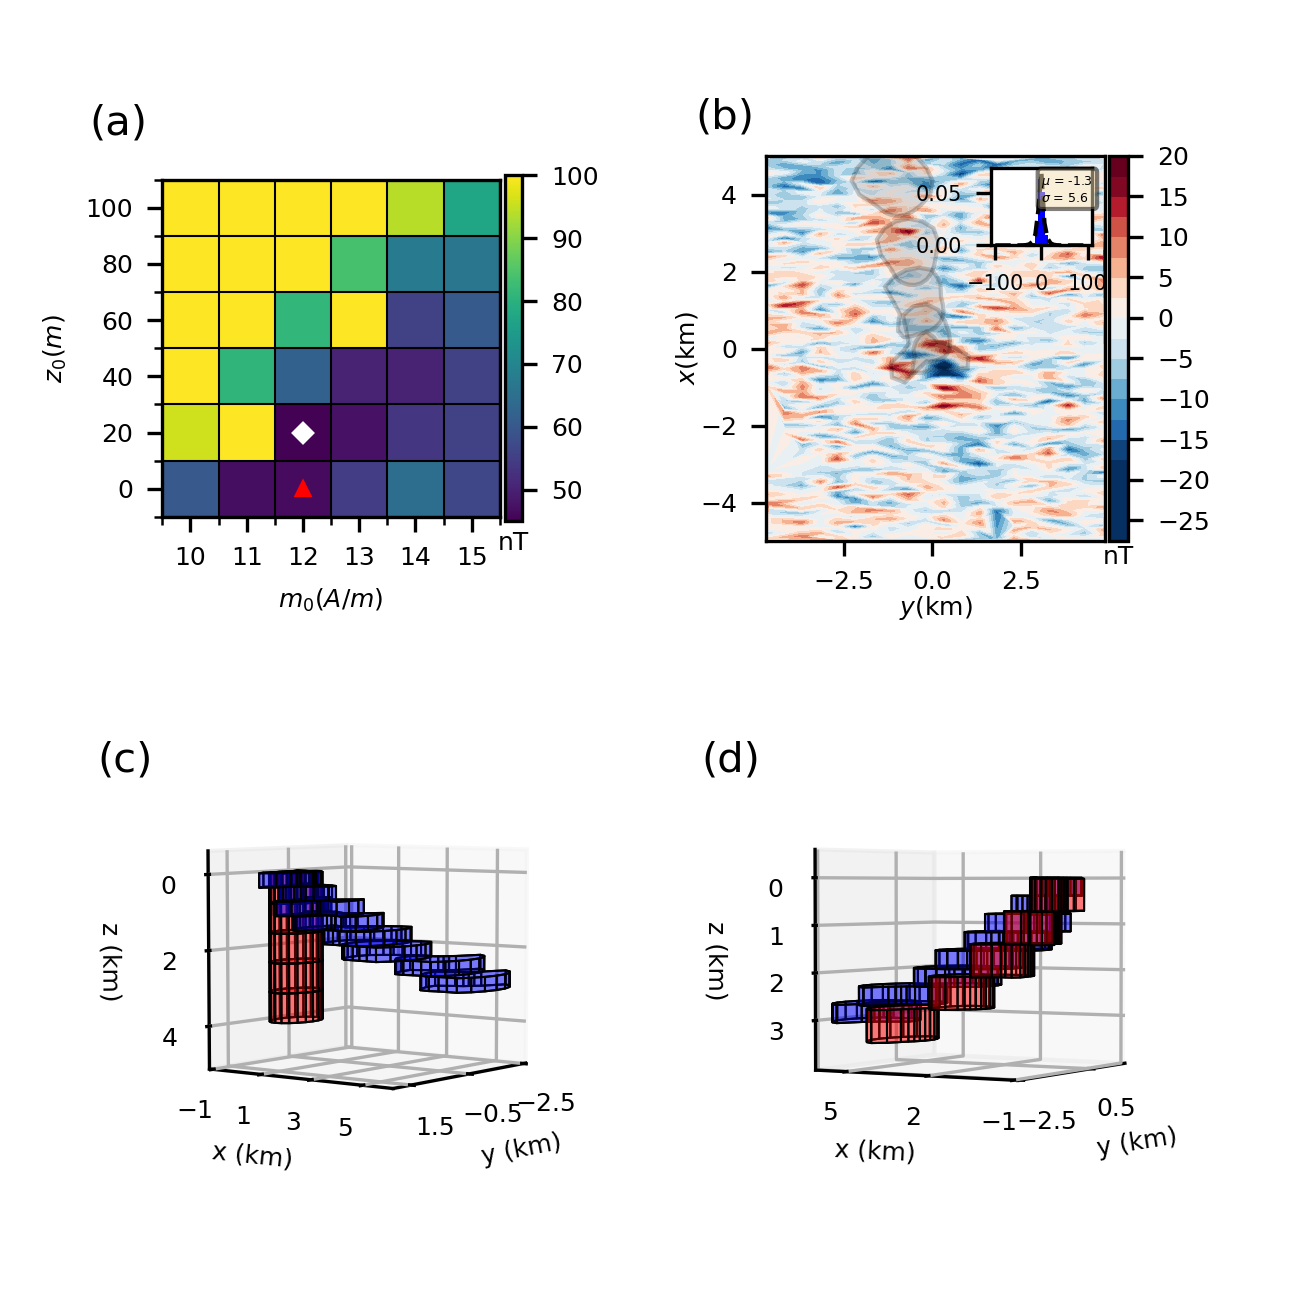
\includegraphics[width=\textwidth]{inclined-l2-solution.png}
	\caption{Soluções L2 obtidas para o modelo inclinado. 
		(a) Mapa discreto da função objetivo produzida pelos modelos obtidos a partir da varredura de valores de profundidade do topo $z_{0}$ e intensidade de magnetização total $m_{0}$. 
		O triângulo vermelho representa os valores verdadeiros para $m_{0}$ e $z_{0}$, assim como os valores que definem a melhor solução L2.
		(b) Resíduos entre os dados contaminados com ruído (Figura \ref{fig:inclined_model}a) 
		e os dados preditos (não mostrados) produzidos pela melhor solução L2 (prismas vermelhos no painel d). 
		O histograma dos resíduos inserido em (b) mostra a curva Gaussiana ajustada (linha tracejada).
		Os polígonos cinzas representam as projeções horizontais de todos os prismas que compõe a melhor solução. 
		(c) e (d) Visualização em perspectiva da aproximação inicial (prismas vermelhos) e 
		a melhor solução (prismas vermelhos), respectivamente. Os prismas azuis são o modelo da fonte alvo. 
	}
	\label{fig:inclined_l2_result}
\end{figure}
\pagebreak
\begin{figure}[!htb]
	\centering
	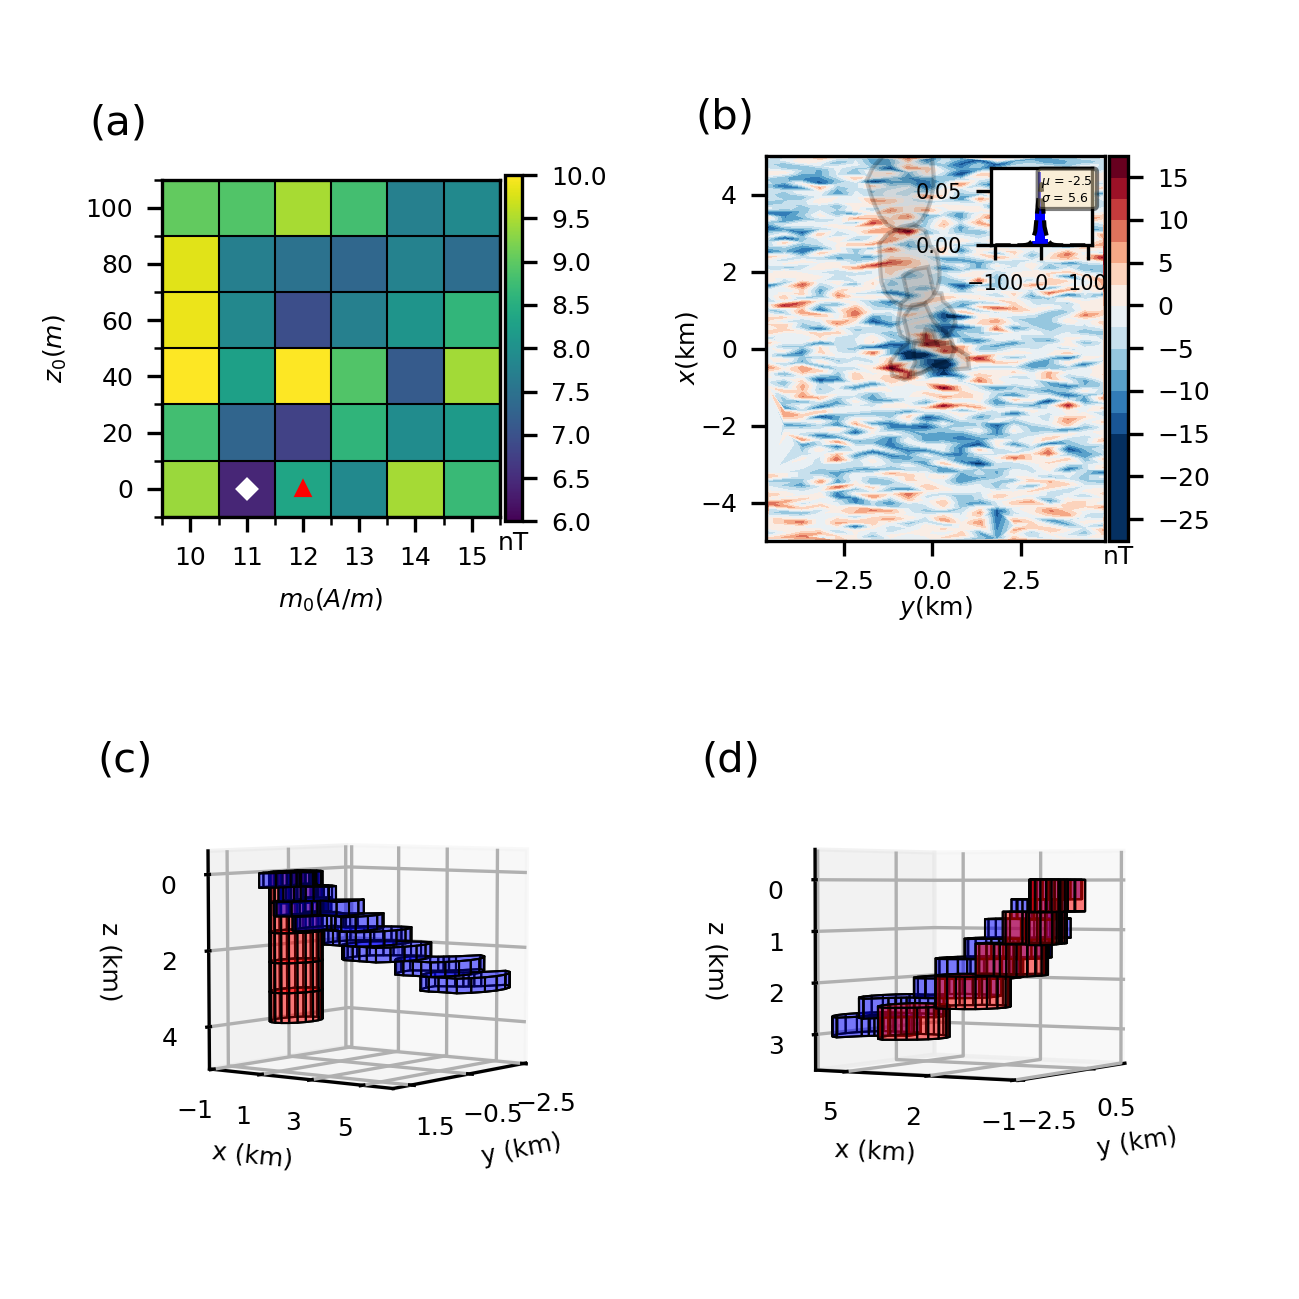
\includegraphics[width=\textwidth]{inclined-l1-solution.png}
	\caption{Soluções L1 obtidas para o modelo inclinado. 
		(a) Mapa discreto da função objetivo produzida pelos modelos da malha de varredura para valores de profundidade do topo $z_{0}$ e intensidade de magnetização total $m_{0}$. 
		O triângulo vermelho representa os valores verdadeiros para $m_{0}$ e $z_{0}$, assim como os valores que definem a melhor solução L1.
		(b) Resíduos entre os dados contaminados com ruído (Figura \ref{fig:inclined_model}a) 
		e os dados preditos (não mostrados) produzidos pela melhor solução L1 (prismas vermelhos no painel d). 
		O histograma dos resíduos inserido em (b) mostra a curva Laplaciana ajustada (linha tracejada).
		Os polígonos cinzas representam as projeções horizontais de todos os prismas que compõe a melhor solução. 
		(c) e (d) Visualização em perspectiva da aproximação inicial (prismas vermelhos) e 
		a melhor solução (prismas vermelhos), respectivamente. Os prismas azuis são o modelo da fonte alvo. 
	}
	\label{fig:inclined_l1_result}
\end{figure}
\pagebreak

\section{Modelo inclinado com regional}

Este teste tem o objetivo de testar o método em uma situação muito comum em um estudo com dados reais: a presença de um campo regional.
Para simular essa situação, a anomalia de campo total produzida pelo modelo inclinado (Figura \ref{fig:inclined_model}a) foi calculada em uma área maior e somada a um campo regional gerado através de um polinômio de primeira ordem (Fgiuras \ref{fig:great_data}a e \ref{fig:great_data}b).
A partir desses dados, foi estimado um polinômio de primeira ordem por meio do método de mínimos quadrados (Figura \ref{fig:great_data}c) a fim de remover a influência do campo regional da anomalia de campo total (Figura \ref{fig:great_data}a).
Embora a direção do campo regional estimado (Figura \ref{fig:great_data}d) tenha uma direção diferente da verdadeira (Figura \ref{fig:great_data}b), ele recupera muito bem sua amplitude.
A Figura \ref{fig:great_model_rtp}a mostra a anomalia de campo total residual obtida pela remoção do campo regional estimado (Figura \ref{fig:great_data}d) e a Figura \ref{fig:great_model_rtp}b mostra que os resíduos entre a anomalia de campo total residual e a verdadeira (Figuras \ref{fig:great_model_rtp}a e \ref{fig:inclined_model}a) se comportam como ruído, o que indica um bom ajuste dos dados.
O método foi aplicado para inverter a anomalia de campo total residual (Figura \ref{fig:great_model_rtp}a) e obter soluções L2 e L1.
Para cada tipo de solução, foram geradas $36$ soluções L2 e $36$ soluções L1, 
todas elas foram obtidas com a mesma malha de varredura $6 \times 6$ de profundidades do topo $z_{0}$ e intensidade de magnetização total $m_{0}$.
A melhor solução L2 e L1 são definidas como aquelas que produzem o menor valor da função objetivo para cada caso.

A Figura \ref{fig:great_model_rtp}c mostra a anomalia RTP obtida a partir da anomalia de campo total residual (Figura \ref{fig:great_model_rtp}a) e 
a projeção horizontal das aproximações iniciais $\hat{\mathbf{p}}_{(0)}$ 
usadas nas sucessivas inversões (Figuras \ref{fig:great_l2_result} e 
\ref{fig:great_l1_result}).
As aproximações iniciais são compostas de $ L= 5$ prismas com $ V = 20 $ vértices, mesma direção de magnetização do corpo verdadeiro, espessura $ dz=350 $ m e centro em $ (x_0, y_0) = (-200, 0) $.
A Figura \ref{fig:great_l2_result}a mostra que a melhor solução L2 obtida superestima tanto a profundidade do topo $z_{0}$ quanto o valor da intensidade de magnetização total $m_{0}$ verdadeira. Essa solução L2 produz um bom ajuste dos dados (Figura \ref{fig:great_l2_result}b), possui uma profundidade da base em $3063.2$ m e também recupera a geometria do corpo verdadeiro (Figura \ref{fig:great_l2_result}d).
A Figura \ref{fig:great_l1_result} mostra um resultado similar em relação a geometria, porém superestima menos os valores de profundidade do topo $z_{0}$ quanto o valor da intensidade de magnetização total $m_{0}$. A profundidade da base estimada foi de $2912.3$ m que é um pouco inferior à estimada pela solução L2.
Podemos observar que nesse teste ambas as abordagens L2 e L1 foram bem sucedidas em estimar a forma do corpo e recuperam as feições principais da fonte alvo. Entretanto, nesse caso, a solução L1 foi ligeiramente superior à solução L2 na estimativa de $ z_0 $ e $ m_0 $.
Todas as soluções L2 produzidas neste teste foram obtidas usando o seguinte conjunto de pesos normalizados $\tilde{\alpha}_{\ell}$ (Equação \ref{eq:alphas}): 
$\tilde{\alpha}_{1} = 10^{-3}$, $\tilde{\alpha}_{2} = 10^{-3}$, 
$\tilde{\alpha}_{3} = 10^{-6}$, $\tilde{\alpha}_{4} = 10^{-6}$, e 
$\tilde{\alpha}_{5} = 10^{-5}$. 
Já as soluções L1 foram obtidas utilizando o conjunto: 
$\tilde{\alpha}_{1} = 10^{-4}$, $\tilde{\alpha}_{2} = 10^{-4}$, 
$\tilde{\alpha}_{3} = 10^{-6}$, $\tilde{\alpha}_{4} = 10^{-6}$, e 
$\tilde{\alpha}_{5} = 10^{-5}$.
É importante notar que, mesmo a solução L1 sendo superior à L2, não há diferenças significativas entre as soluções L2 e L1 obtidas pelo método.

\begin{figure}[!htb]
	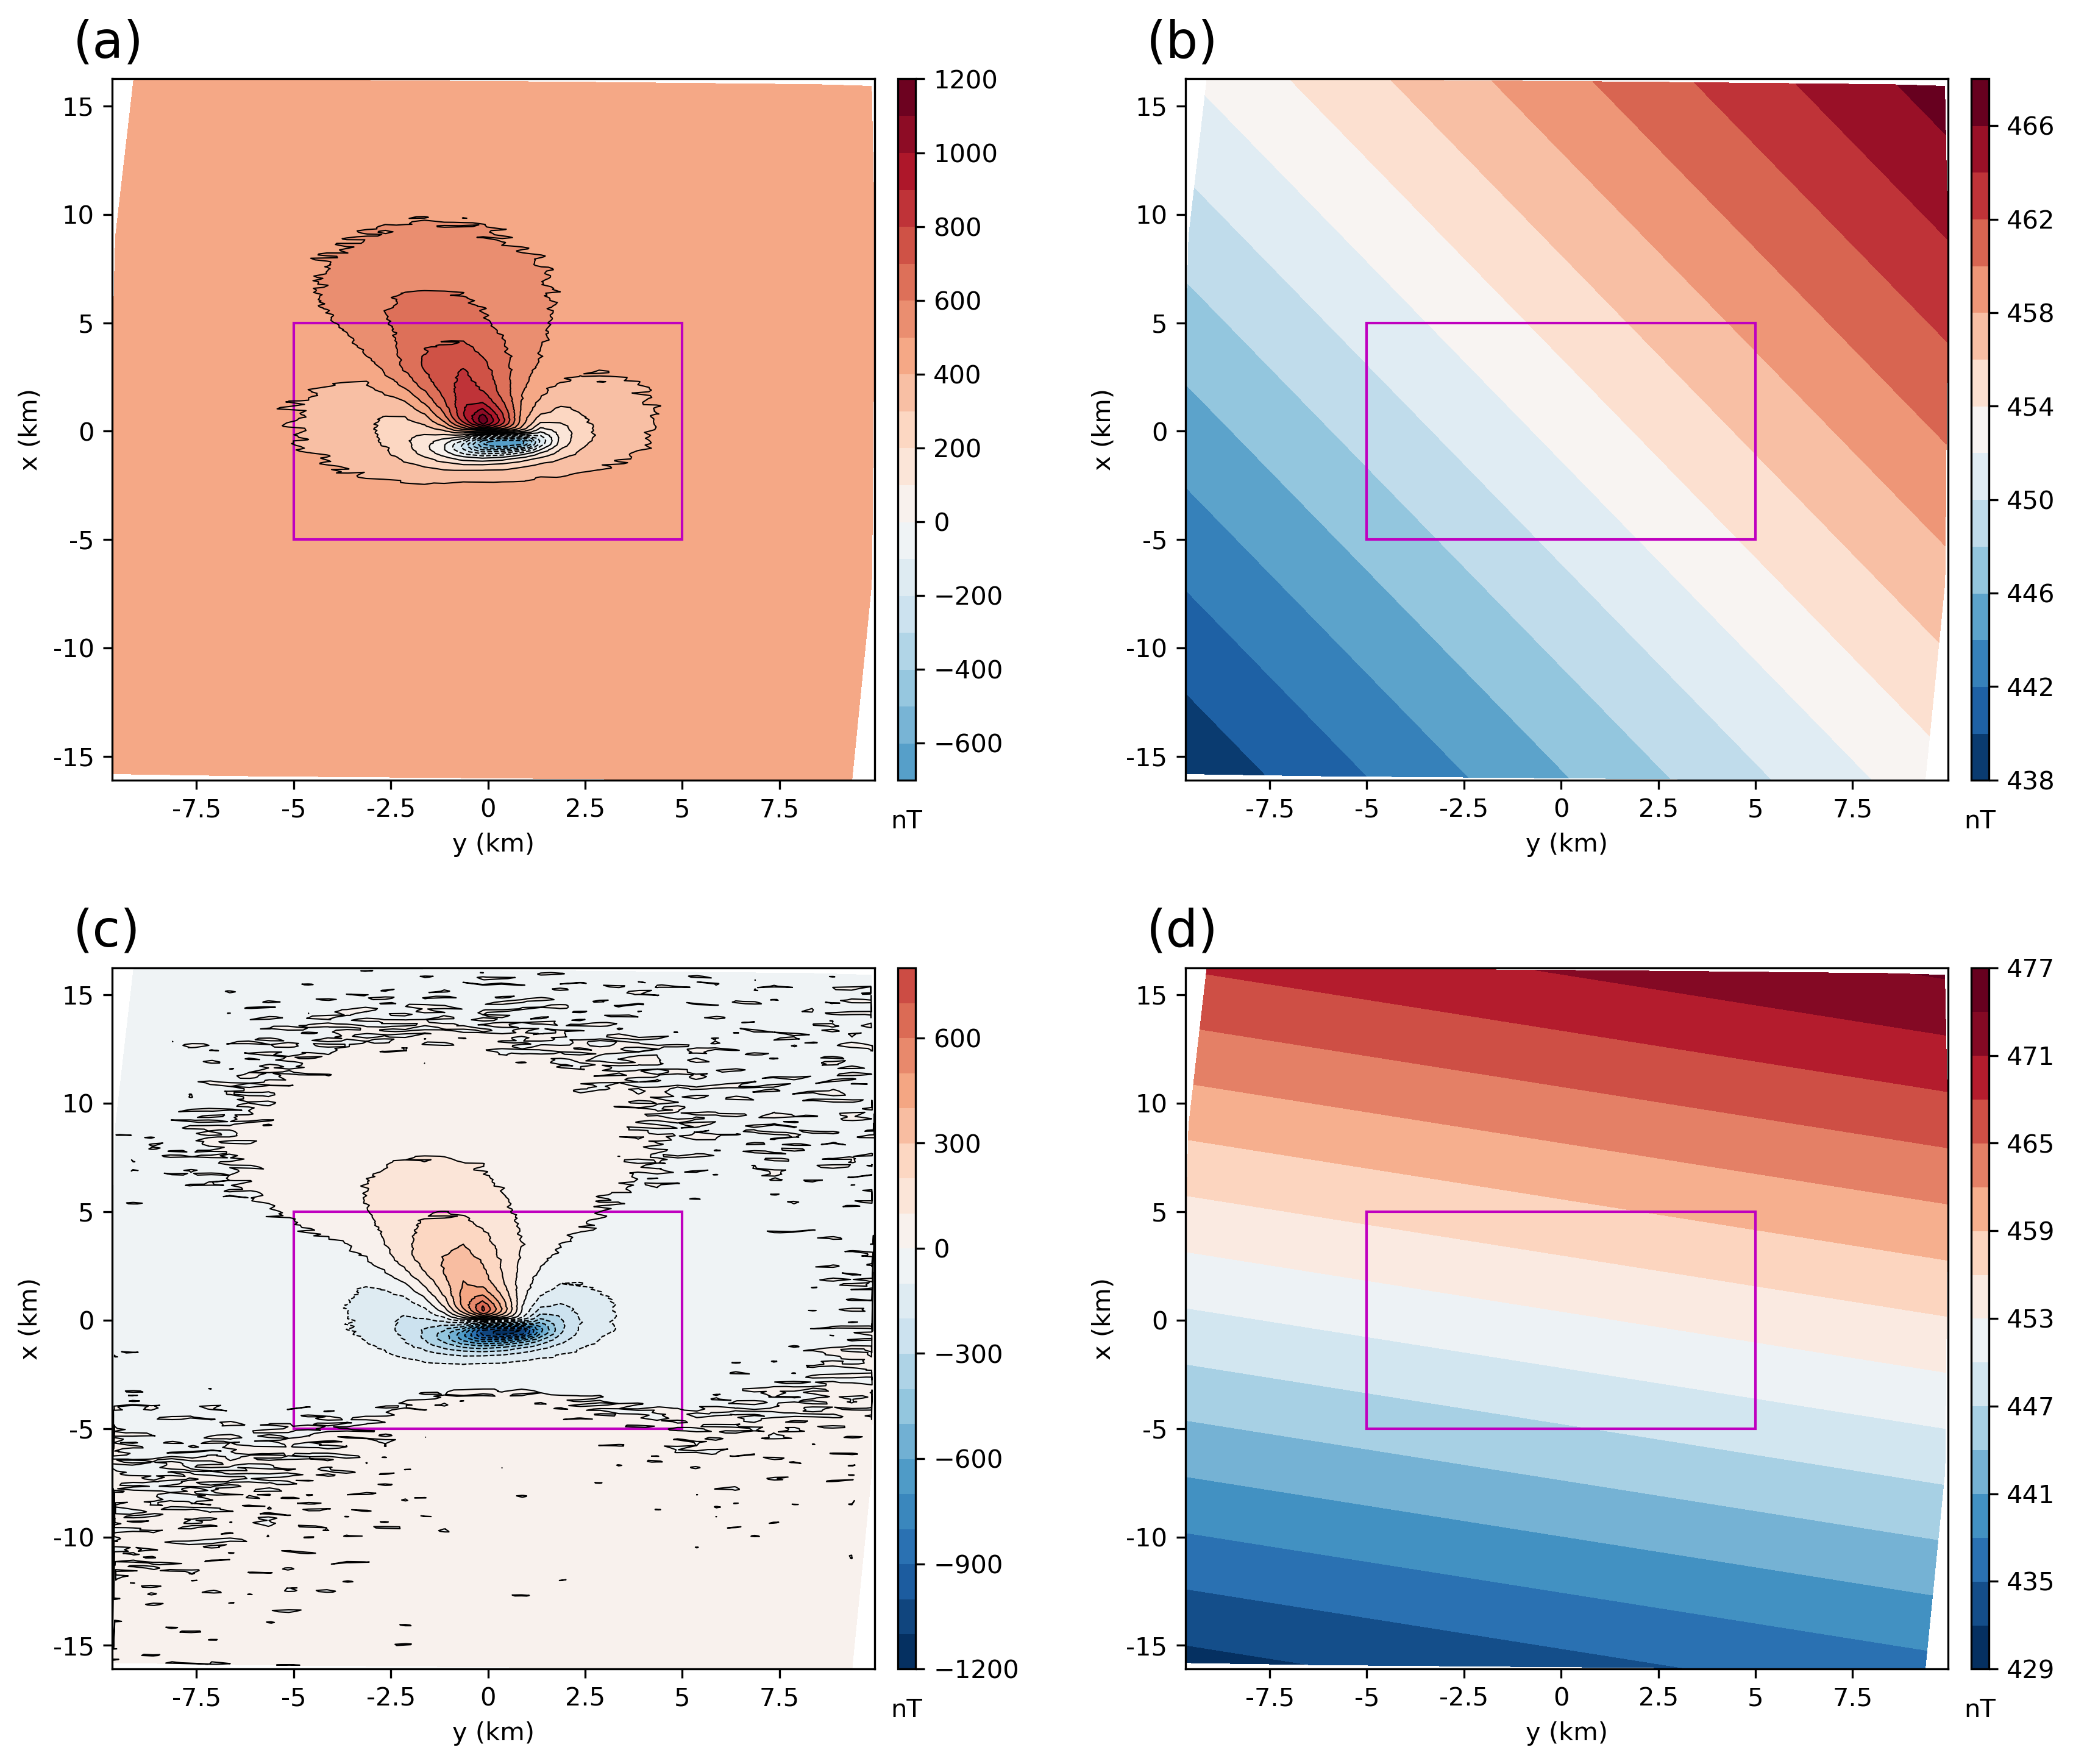
\includegraphics[width=\textwidth]{inclined-data-large.png}
	\caption{Aplicação aos dados do modelo inclinado com regional. 
		(a) Anomalia de campo total produzida pela modelo inclinado (Figura \ref{fig:inclined_model}a) somada a um campo regional sintético (painel b).
		(b) Polinômio de primeira ordem que representa o campo regional sintético.
		(c) Anomalia de campo total residual obtida pela diferença entre (a) e (d). (d) Campo regional estimado por um polinômio simples através de mínimos quadrados.
	}
	\label{fig:great_data}
\end{figure}
\pagebreak

\pagebreak

\begin{figure}[!htb]
	\centering
	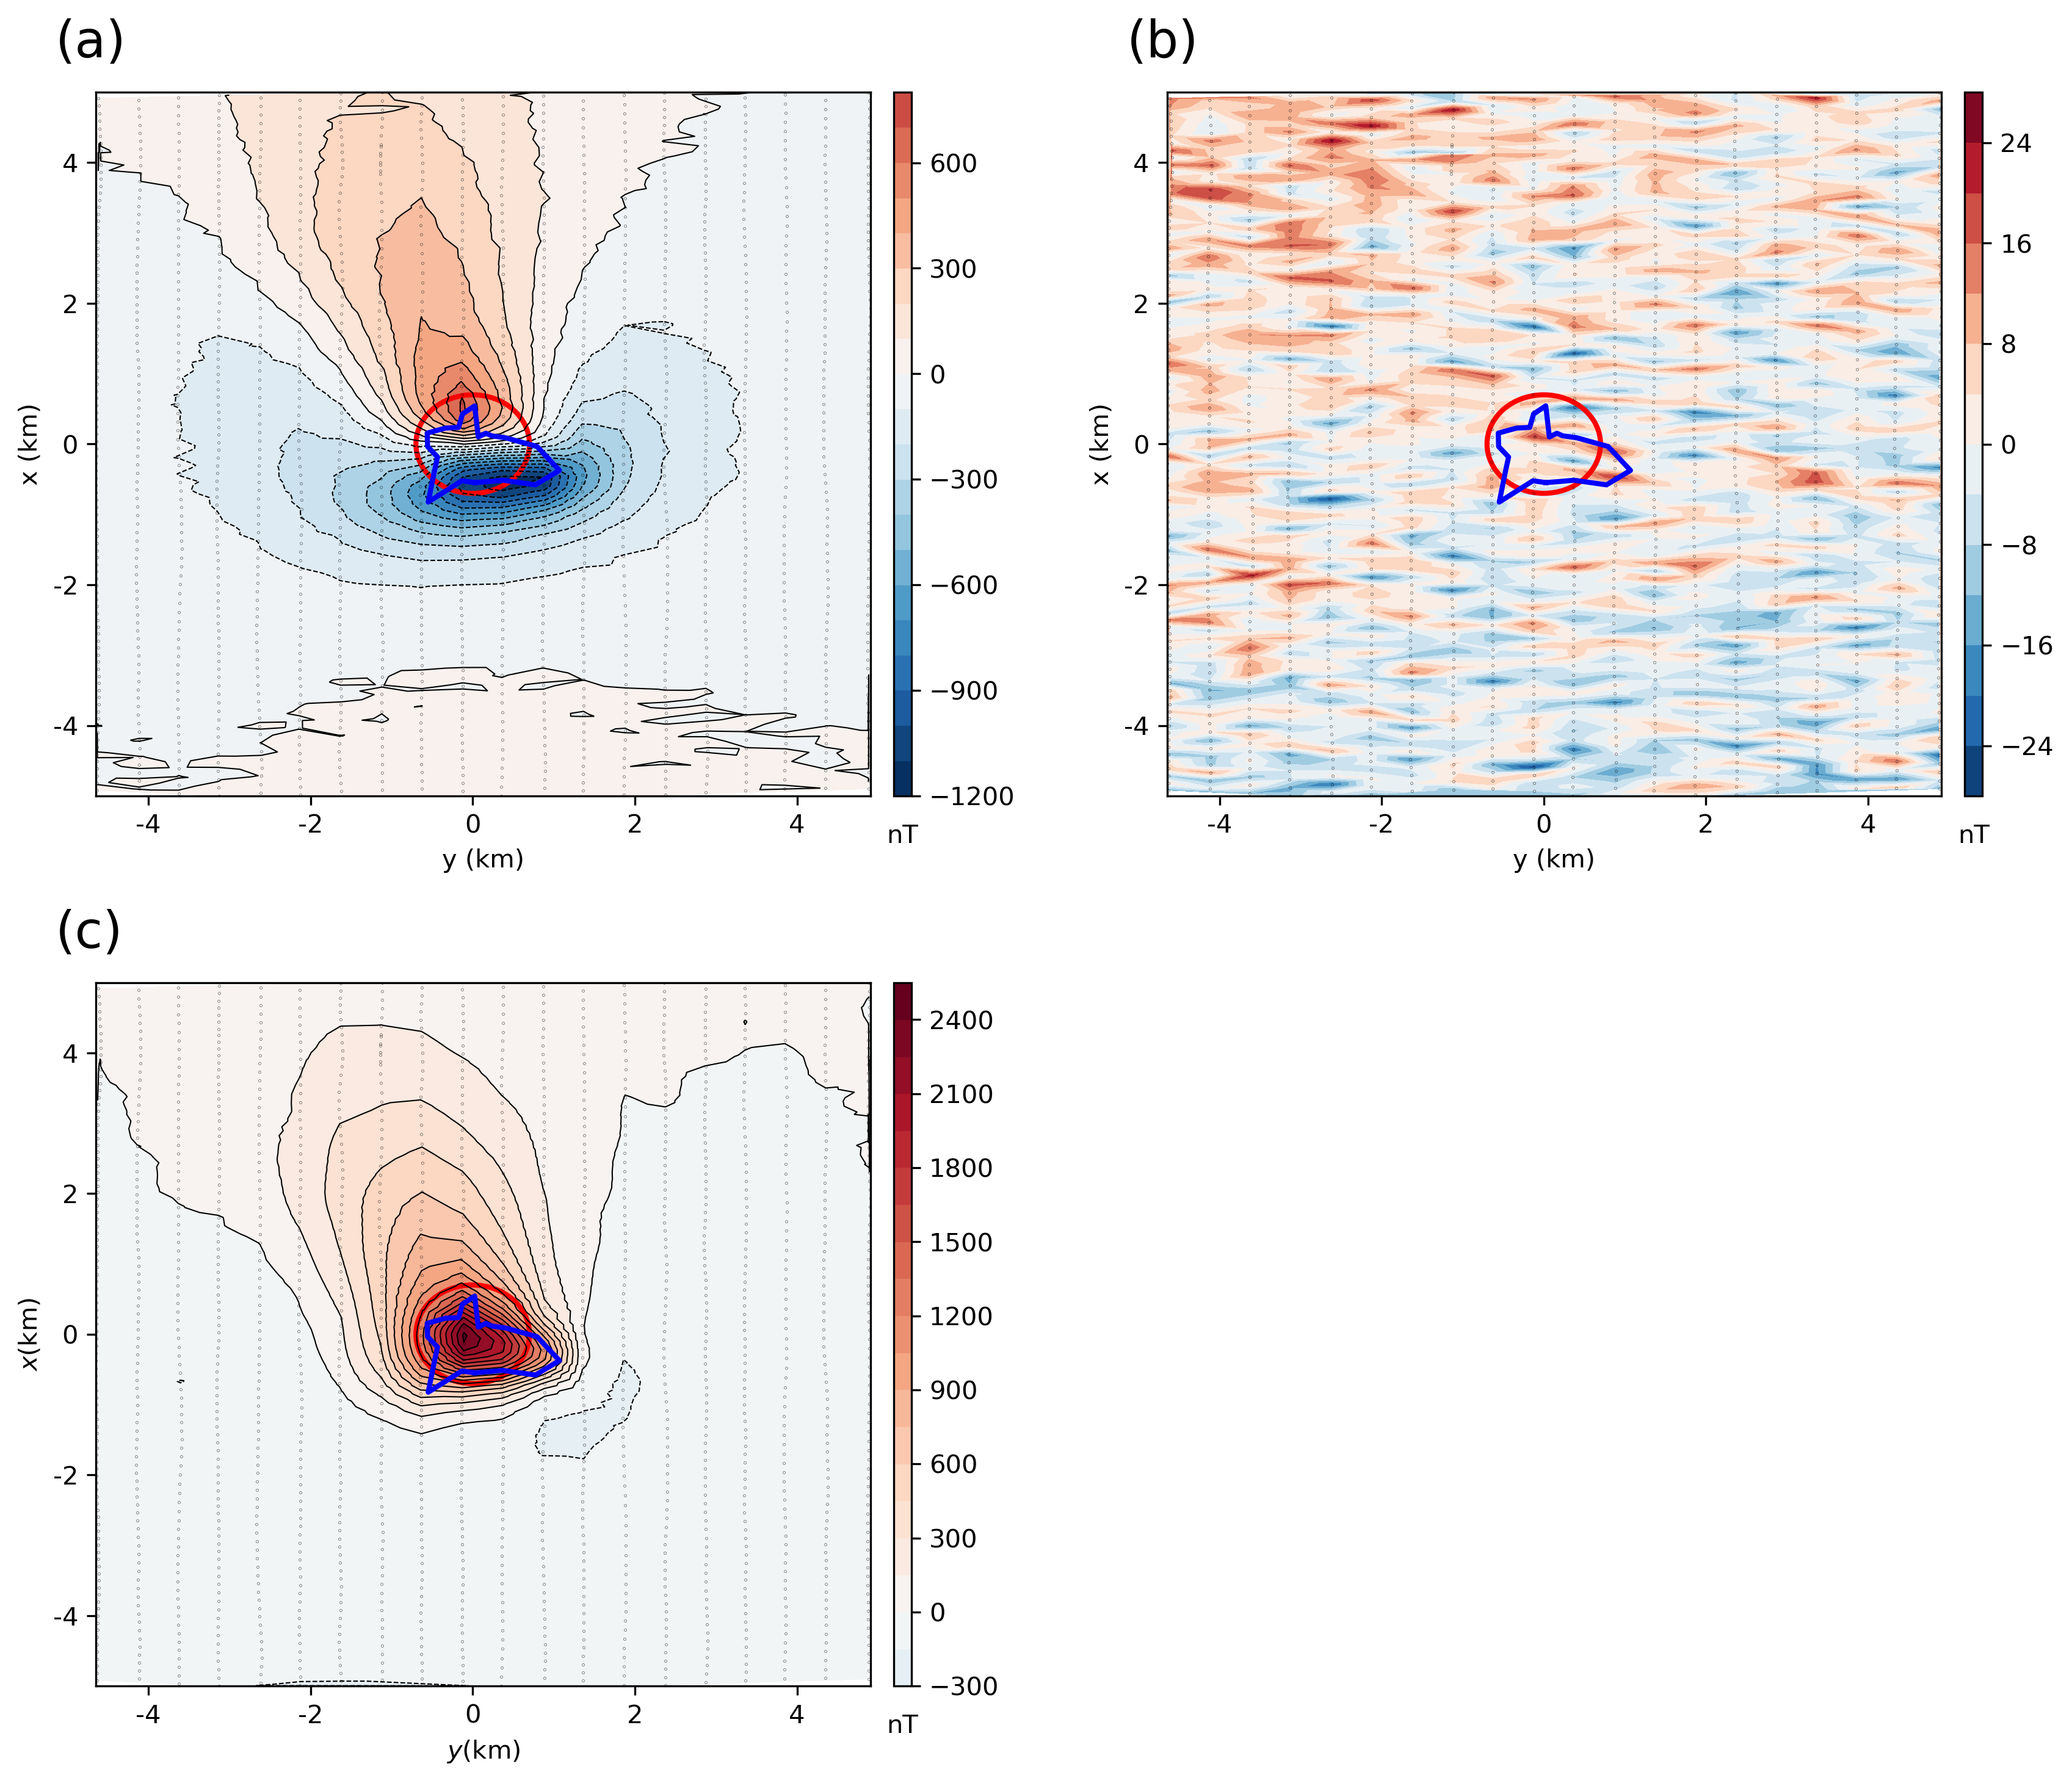
\includegraphics[width=\textwidth]{great_rtp.png}
	\caption{Aplicação aos dados do modelo inclinado com regional. 
		(a) Anomalia de campo total residual contida no retângulo rosa na Figura \ref{fig:great_data}c. (b) Resíduos obtidos pela diferença entre as anomalias de campo total gerada no teste anterior (Figrura \ref{fig:inclined_model}a) e a residual (painel a). (c) Anomalia RTP sobre a área de estudo. Ambos painéis são limitados pelo retângulos rosa na Figura \ref{fig:great_data}. As linhas azuis e vermelhas correspondem, respectivamente, às projeções horizontais da porção mais rasa da fonte alvo e da aproximação inicial utilizada nas inversões subsequentes (prismas vermelhos nas Figuras \ref{fig:great_l2_result}c e 
		\ref{fig:great_l1_result}c).
	}
	\label{fig:great_model_rtp}
\end{figure}

\pagebreak

\begin{figure}[!htb]
	\centering
	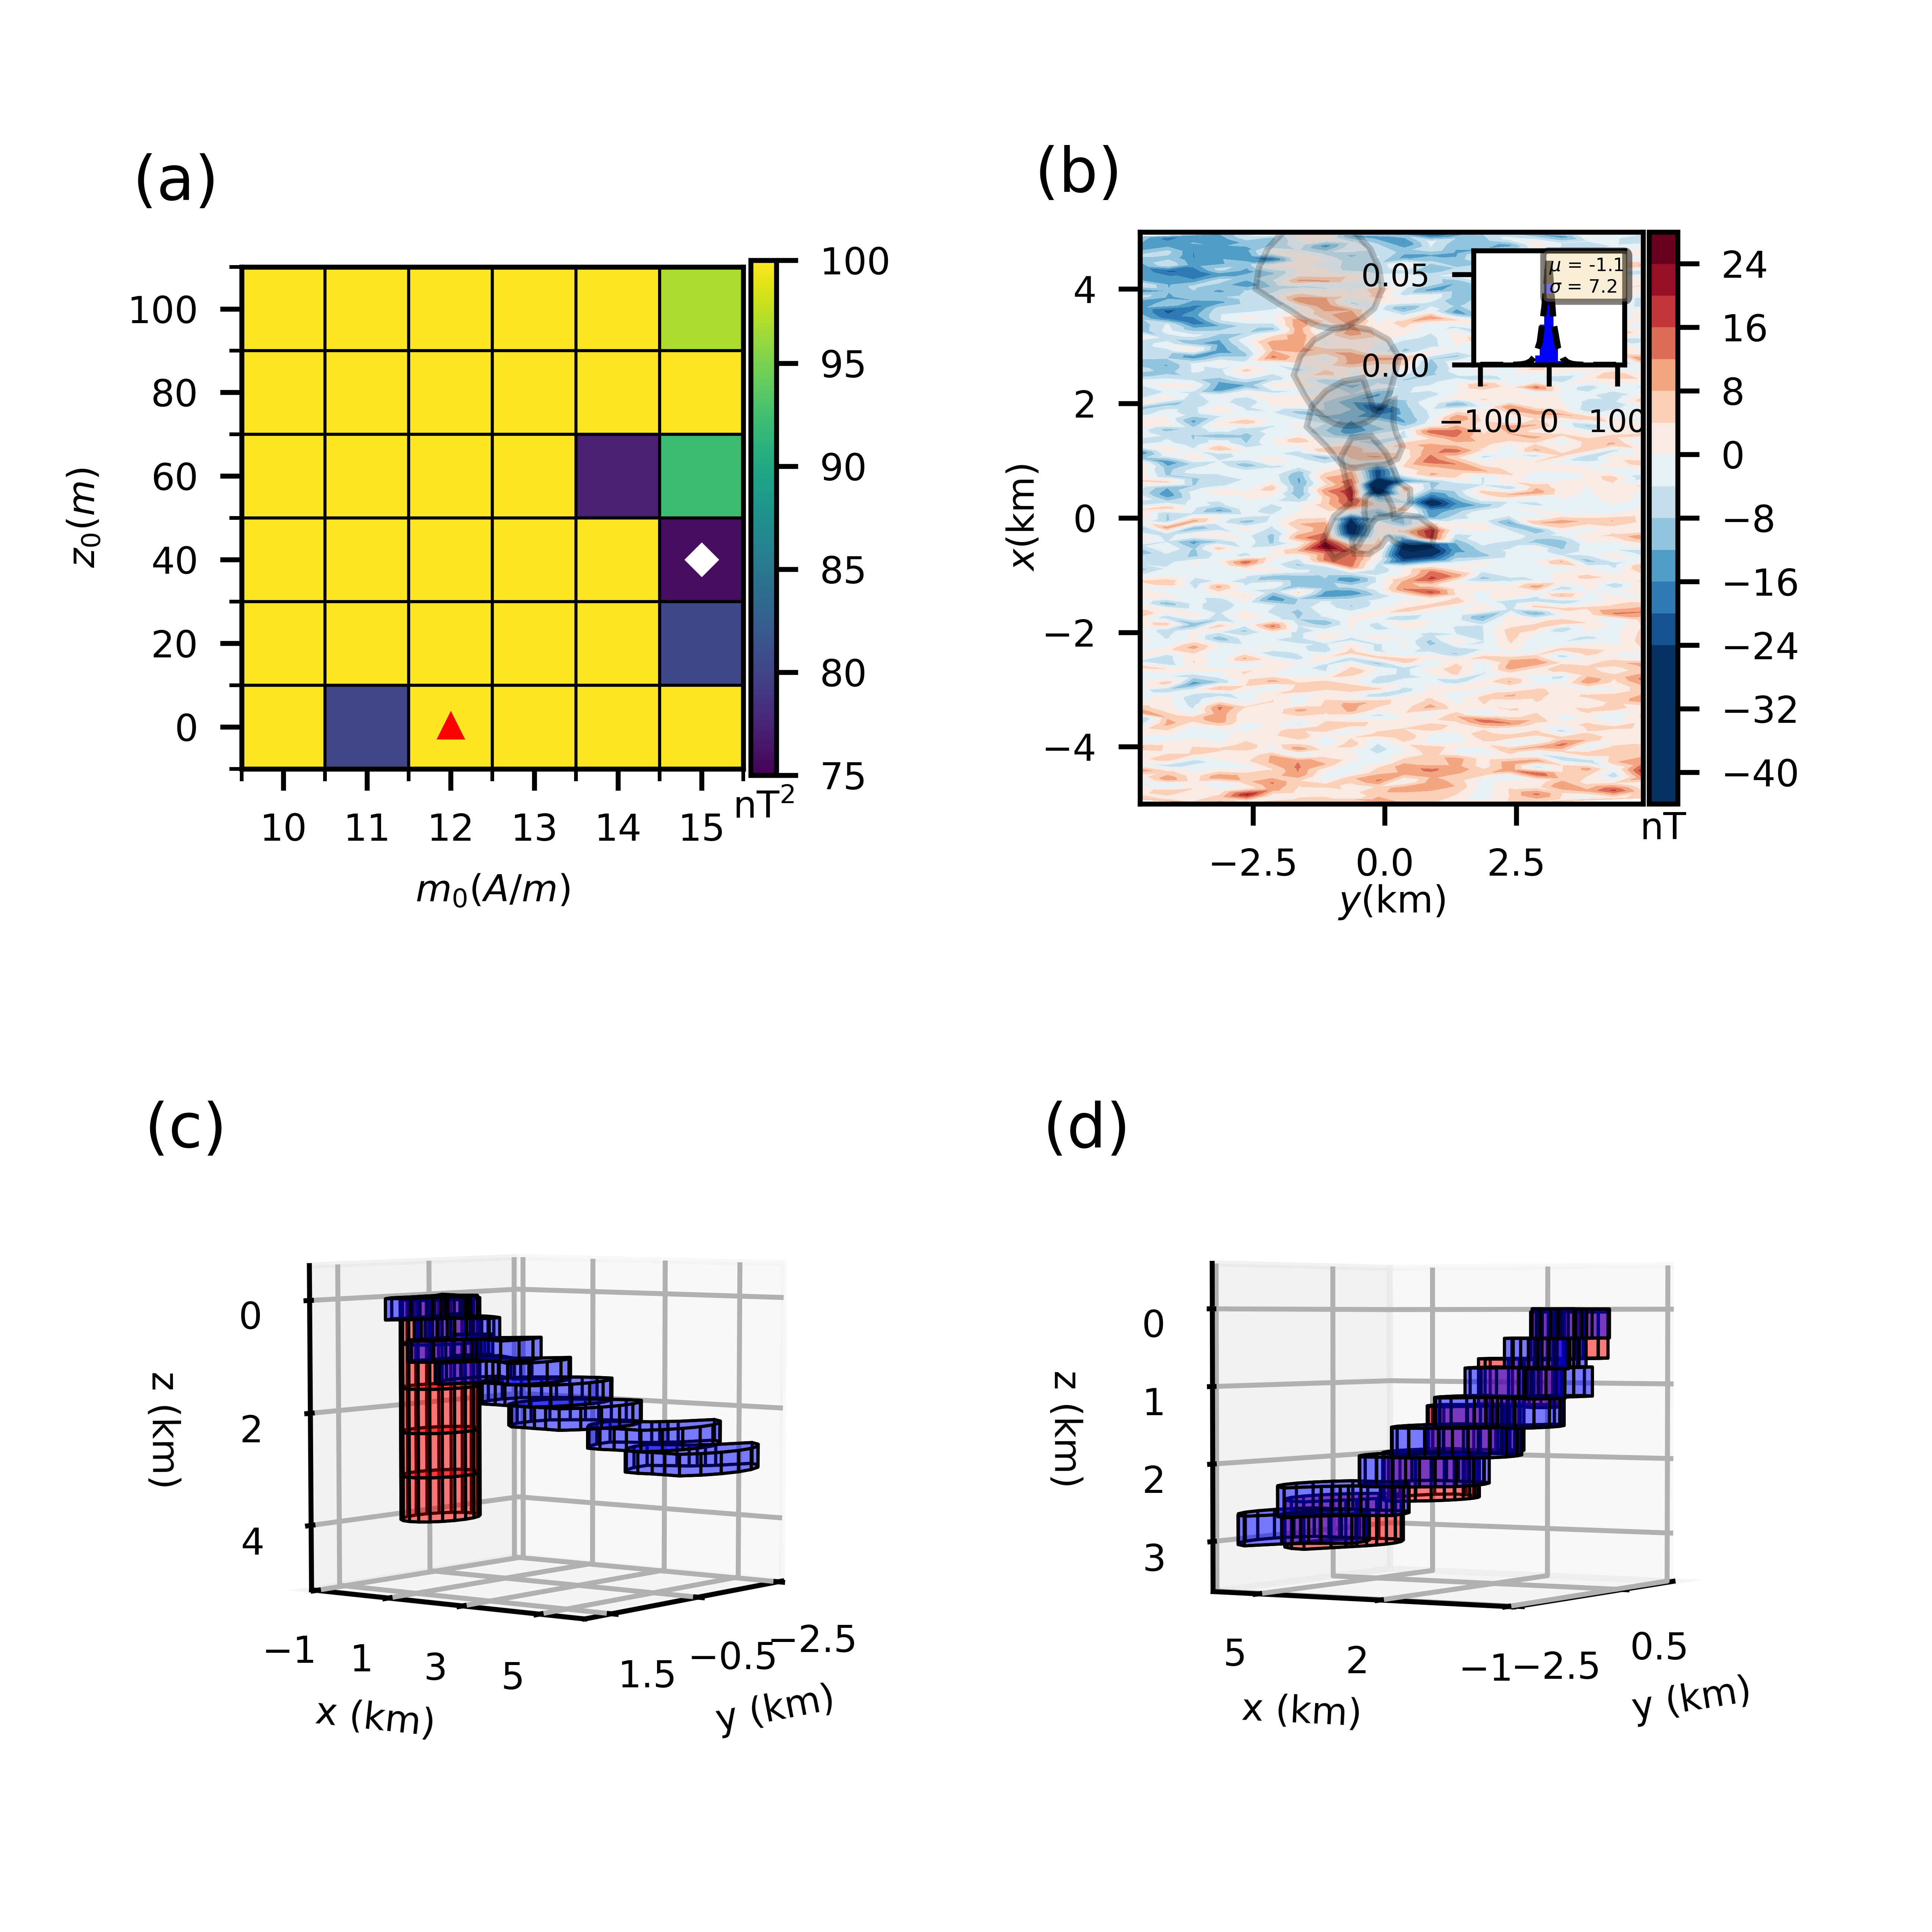
\includegraphics[width=\textwidth]{great-l2-solution.png}
	\caption{Soluções L2 obtidas para o modelo inclinado com regional. 
		(a) Mapa discreto da função objetivo produzida pelos modelos obtidos a partir da varredura de valores de profundidade do topo $z_{0}$ e intensidade de magnetização total $m_{0}$. 
		O triângulo vermelho representa os valores verdadeiros para $m_{0}$ e $z_{0}$ eo losango branco indica os valores que definem a melhor solução L2.
		(b) Resíduos entre a anomalia de campo total residual (Figura \ref{fig:great_model_rtp}a) 
		e os dados preditos (não mostrados) produzidos pela melhor solução L2 (prismas vermelhos no painel d). 
		O histograma dos resíduos inserido em (b) mostra a curva Gaussiana ajustada (linha tracejada).
		Os polígonos cinzas representam as projeções horizontais de todos os prismas que compõe a melhor solução. 
		(c) e (d) Visualização em perspectiva da aproximação inicial (prismas vermelhos) e 
		a melhor solução (prismas vermelhos), respectivamente. Os prismas azuis são o modelo da fonte alvo. 
	}
	\label{fig:great_l2_result}
\end{figure}
\pagebreak
\begin{figure}[!htb]
	\centering
	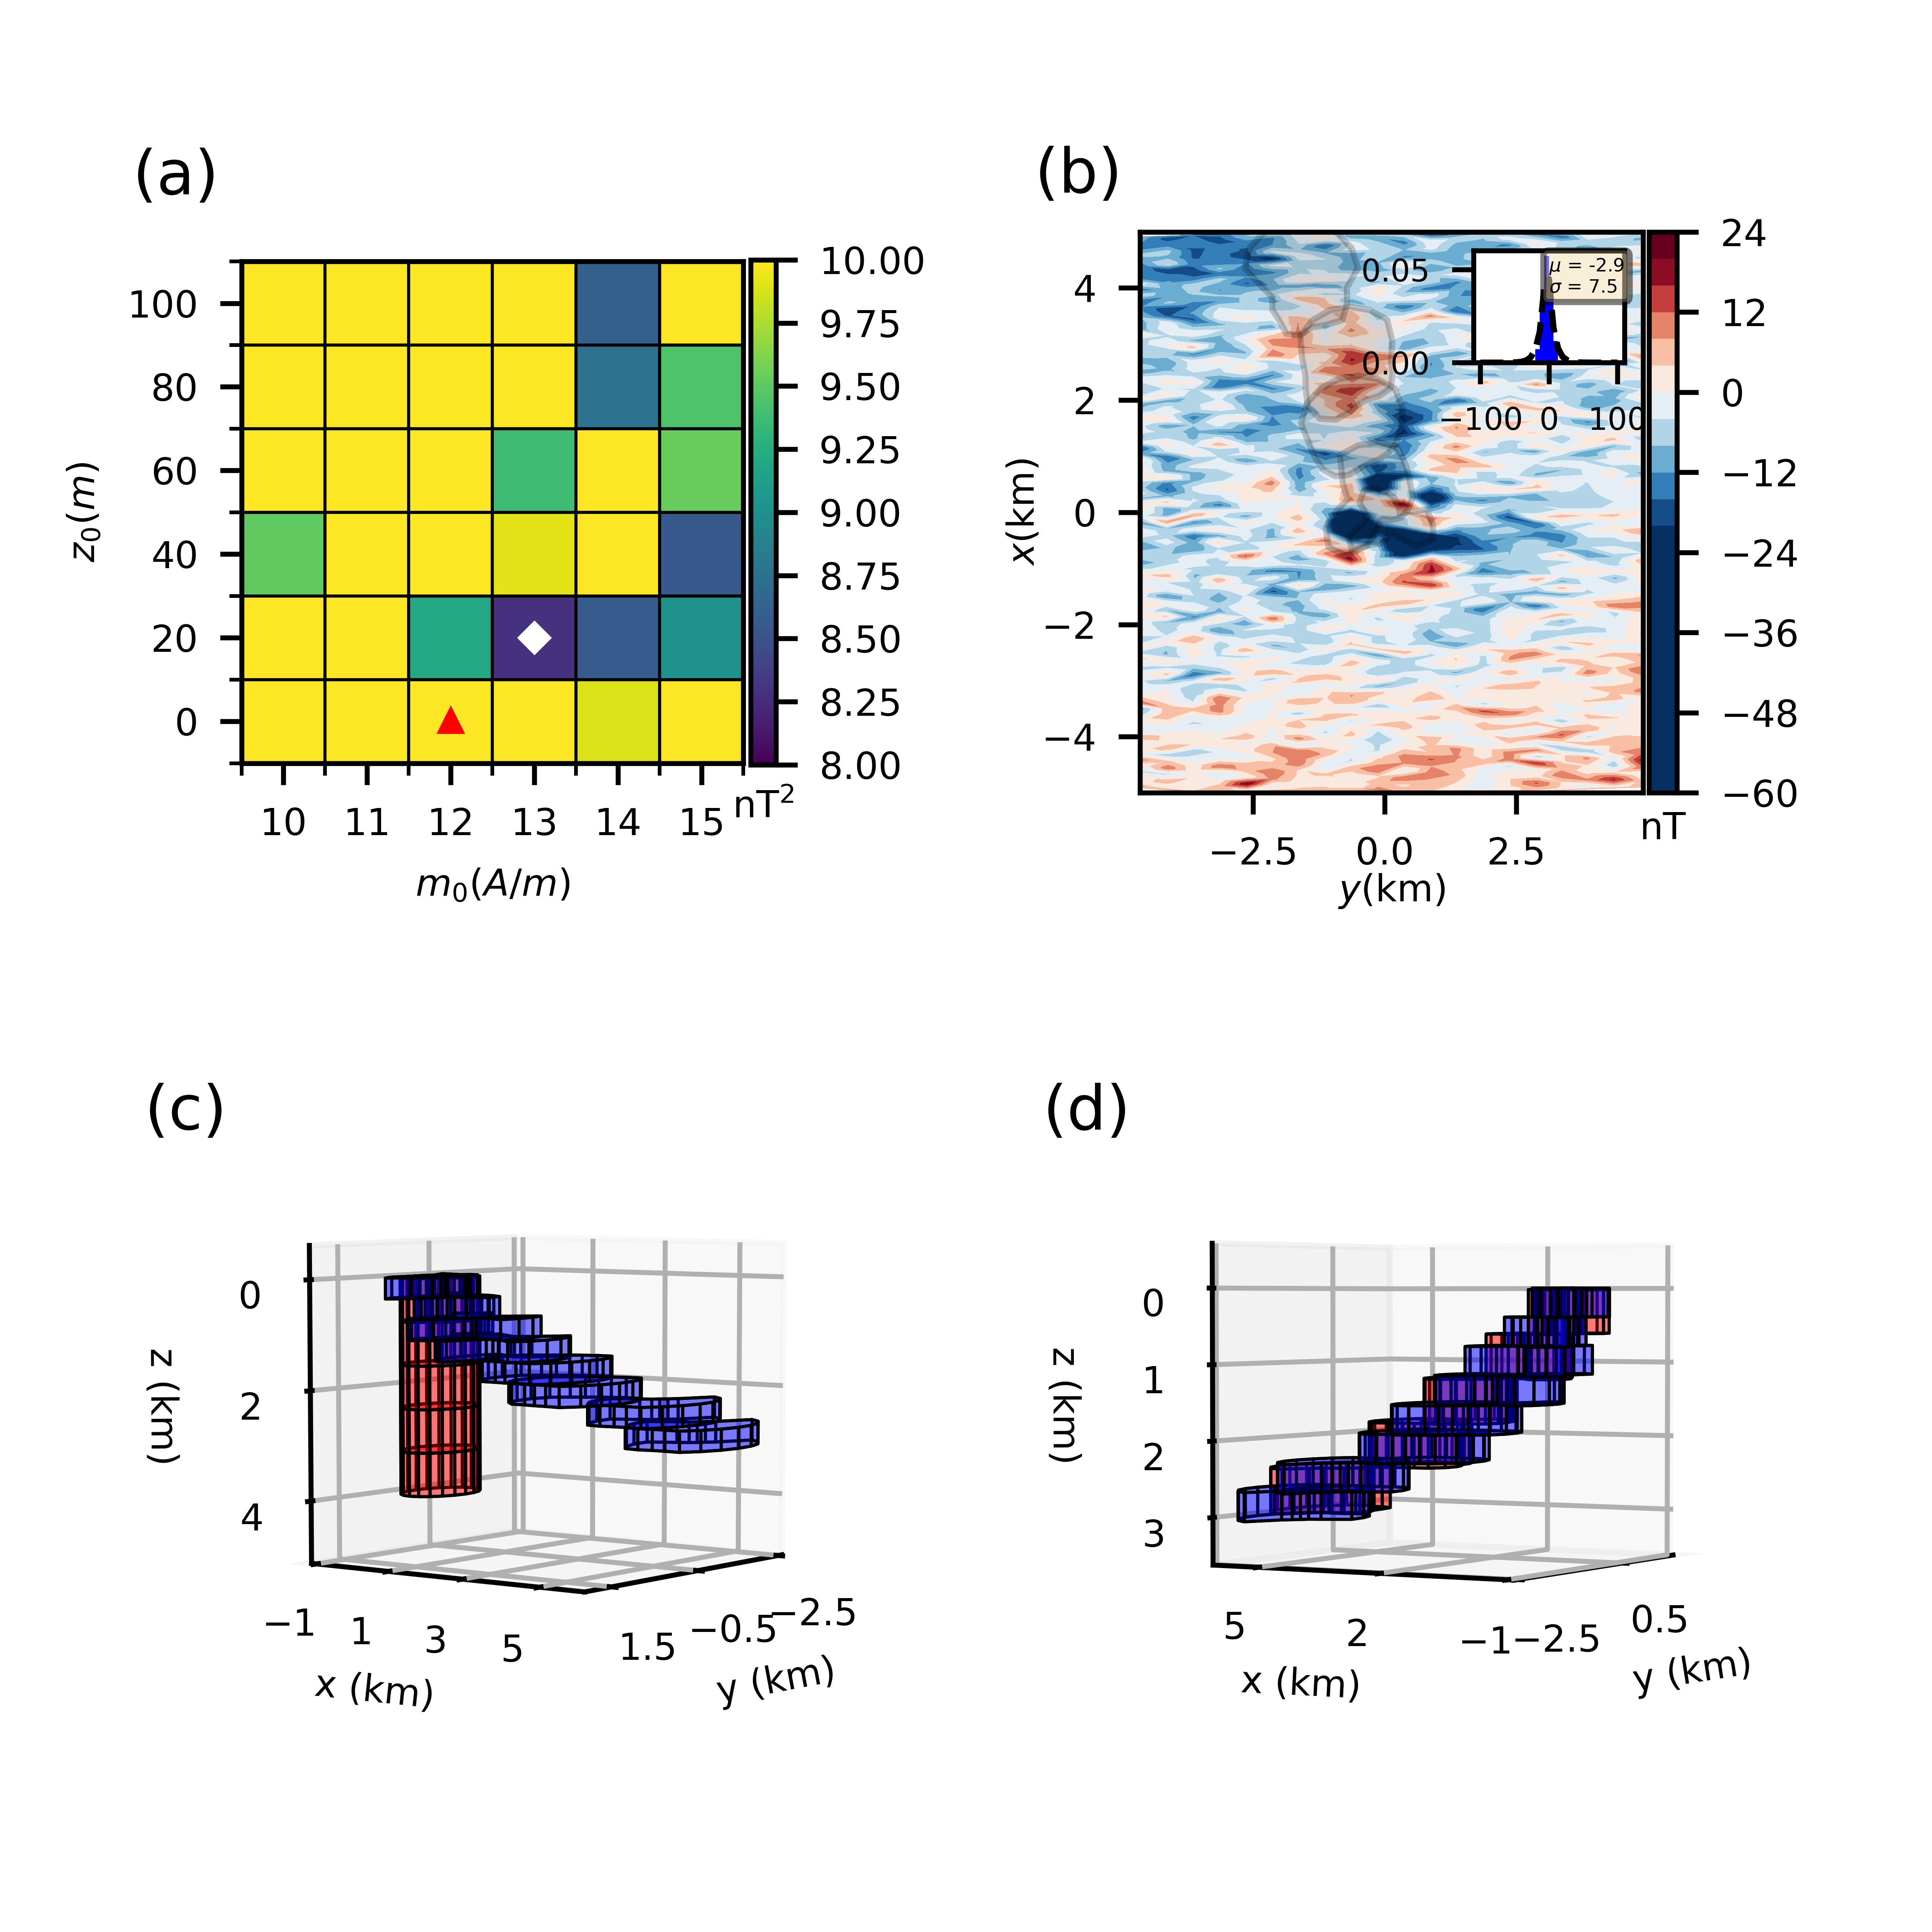
\includegraphics[width=\textwidth]{great-l1-solution.png}
	\caption{Soluções L1 obtidas para o modelo inclinado com regional. 
		(a) Mapa discreto da função objetivo produzida pelos modelos da malha de varredura para valores de profundidade do topo $z_{0}$ e intensidade de magnetização total $m_{0}$. 
		O triângulo vermelho representa os valores verdadeiros para $m_{0}$ e $z_{0}$ e o losango branco indica os valores que definem a melhor solução L1.
		(b) Resíduos entre a anomalia de campo total residual (Figura \ref{fig:great_model_rtp}a) 
		e os dados preditos (não mostrados) produzidos pela melhor solução L1 (prismas vermelhos no painel d). 
		O histograma dos resíduos inserido em (b) mostra a curva Laplaciana ajustada (linha tracejada).
		Os polígonos cinzas representam as projeções horizontais de todos os prismas que compõe a melhor solução. 
		(c) e (d) Visualização em perspectiva da aproximação inicial (prismas vermelhos) e 
		a melhor solução (prismas vermelhos), respectivamente. Os prismas azuis são o modelo da fonte alvo. 
	}
	\label{fig:great_l1_result}
\end{figure}
\pagebreak


\section{Modelo complexo}
\label{sec:target_source_without_interference}

Com o propósito de aplicar o método a problemas mais realistas, foi simulado um corpo geológico complexo imerso em meio não magnético (prismas azuis nas Figuras 
\ref{fig:target_model}, \ref{fig:target_l2_result}, \ref{fig:target_l1_result},
\ref{fig:small_model}, \ref{fig:small_l2_result}, \ref{fig:small_l1_result}, 
\ref{fig:thick_model}, \ref{fig:thick_l2_result}, e \ref{fig:thick_l1_result})
que representa a fonte alvo 3D com profundidade do topo em $130$ m, profundidade da base em $6130$ m, centro em $ (x_0, y_0) = (-250, 250) $ e um vetor de magnetização total constante com inclinação $-50^{\circ}$, 
declinação $9^{\circ}$, e intensidade $12$ A/m. 
Esse modelo é composto de $ 10 $ prismas com seção horizontal irregular com $ 30 $ vértices cada.
Recuperar a geometria desse corpo simulado é uma tarefa complicada porque ele possui um mergulho NO-SE e suas fatias horizontais mostram uma forma que varia ao longo da profundidade, assim, é possível notar que o corpo não satisfaz perfeitamente os vínculos impostos nesse método.
A anomalia de campo total (Figura \ref{fig:target_model}a) produzida pela fonte alvo foi calculada em $1939$ pontos localizados sobre uma superfície ondulada que simula um levantamento aéreo (Figura \ref{fig:target_model}b). Esses dados sintéticos foram contaminados com um ruído Gaussiano pseudo-aleatório de média zero e desvio padrão igual a $5$ nT.
O método foi aplicado para inverter esse dado contaminado com ruído e obter soluções L2 e L1 para três cenários: sem fontes não-alvo, 
com uma fonte não-alvo relativamente pequena e com uma fonte não-alvo relativamente grande.
Para cada cenário, foram geradas $36$ soluções L2 e $36$ soluções L1, 
todas elas foram obtidas com a mesma malha de varredura $6 \times 6$ de profundidades do topo $z_{0}$ e intensidade de magnetização total $m_{0}$.
A melhor solução L2 e L1 são definidas como aquelas que produzem o menor valor da função objetivo para cada caso.

A Figura \ref{fig:target_model_rtp} mostra a anomalia RTP obtida a partir da anomalia de campo total contaminada com ruído (Figura \ref{fig:target_model}a) e 
a projeção horizontal das aproximações iniciais $\hat{\mathbf{p}}_{(0)}$ 
usadas nas sucessivas inversões (Figuras \ref{fig:target_l2_result} e 
\ref{fig:target_l1_result}).
As aproximações iniciais são compostas de $ L= 10$ prismas com $ V = 20 $ vértices, mesma direção de magnetização do corpo verdadeiro, espessura $ dz=650 $ m e centro em $ (x_0, y_0) = (-300, 300) $.
A Figura \ref{fig:target_l2_result}a mostra que a melhor solução L2 foi obtida através dos valores verdadeiros da profundidade do topo $z_{0}$ e intensidade de magnetização total $m_{0}$. Essa solução L2 produz um ótimo ajuste dos dados (Figura \ref{fig:target_l2_result}b), possui uma profundidade da base em $6641.8$ m e também recupera a geometria do corpo verdadeiro (Figura \ref{fig:target_l2_result}d).
A Figura \ref{fig:target_l1_result} mostra um resultado similar produzido pela melhor solução L1, que tem profundidade da base em $6156.5$ m.
O aspecto mais interessante das soluções L2 e L1 obtidas neste teste é que elas recuperam não só as feições principais da fonte mas também seu mergulho e a variação de sua forma ao longo da profundidade.
Todas as soluções L2 e L1 produzidas neste teste foram obtidas usando o seguinte conjunto de pesos normalizados $\tilde{\alpha}_{\ell}$ (Equação \ref{eq:alphas}): 
$\tilde{\alpha}_{1} = 10^{-5}$, $\tilde{\alpha}_{2} = 10^{-4}$, 
$\tilde{\alpha}_{3} = 10^{-4}$, $\tilde{\alpha}_{4} = 10^{-8}$, e 
$\tilde{\alpha}_{5} = 10^{-5}$. 
É importante notar que, devido à ausência de fontes não-alvo neste teste, não há diferenças práticas entre as soluções L2 e L1 obtidas pelo método aqui proposto.


\begin{figure}[!htb]
	\centering
	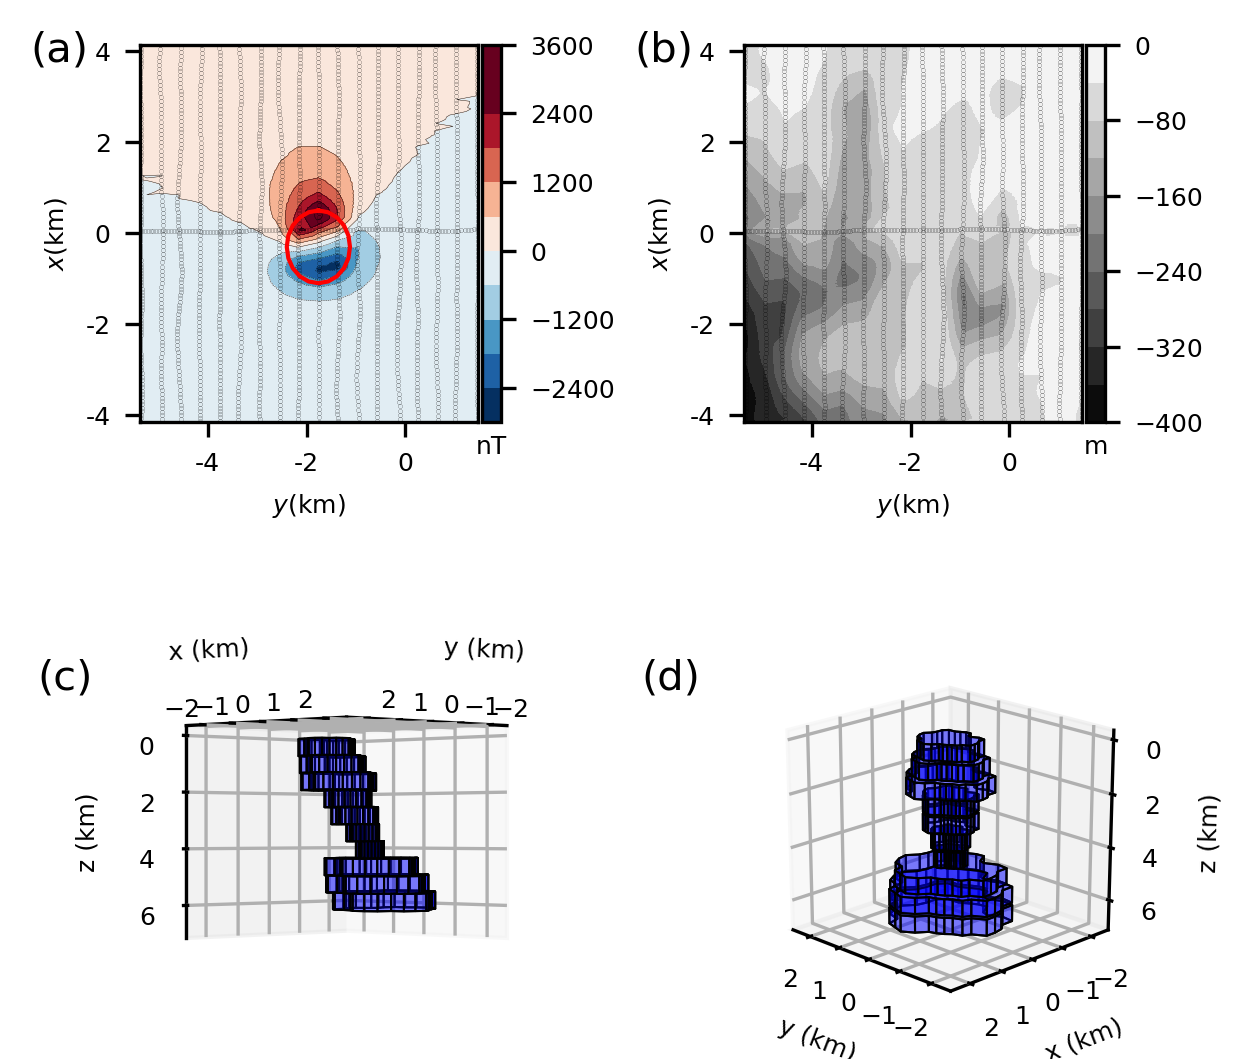
\includegraphics[width=\textwidth]{complex_model_data.png}
	\caption{Modelo da fonte alvo. (a) Anomalia de campo total contaminada com ruído produzida pela fonte alvo (prismas azuis mostrados nos painéis c e d). Os pontos pretos representam os pontos de observação. O círculo vermelho representa a projeção horizontal da aproximação inicial $\hat{\mathbf{p}}_{(0)}$ (prismas vermelhos nas Figuras
		\ref{fig:target_l2_result}c e \ref{fig:target_l1_result}c). (b) Coordenadas verticais dos pontos de observação que simulam um levantamento aéreo.
		(c) e (d) Visualizações em perspectiva do modelo da fonte alvo representada pelos prismas azuis.
	}
	\label{fig:target_model}
\end{figure}
\pagebreak

\begin{figure}[!htb]
	\centering
	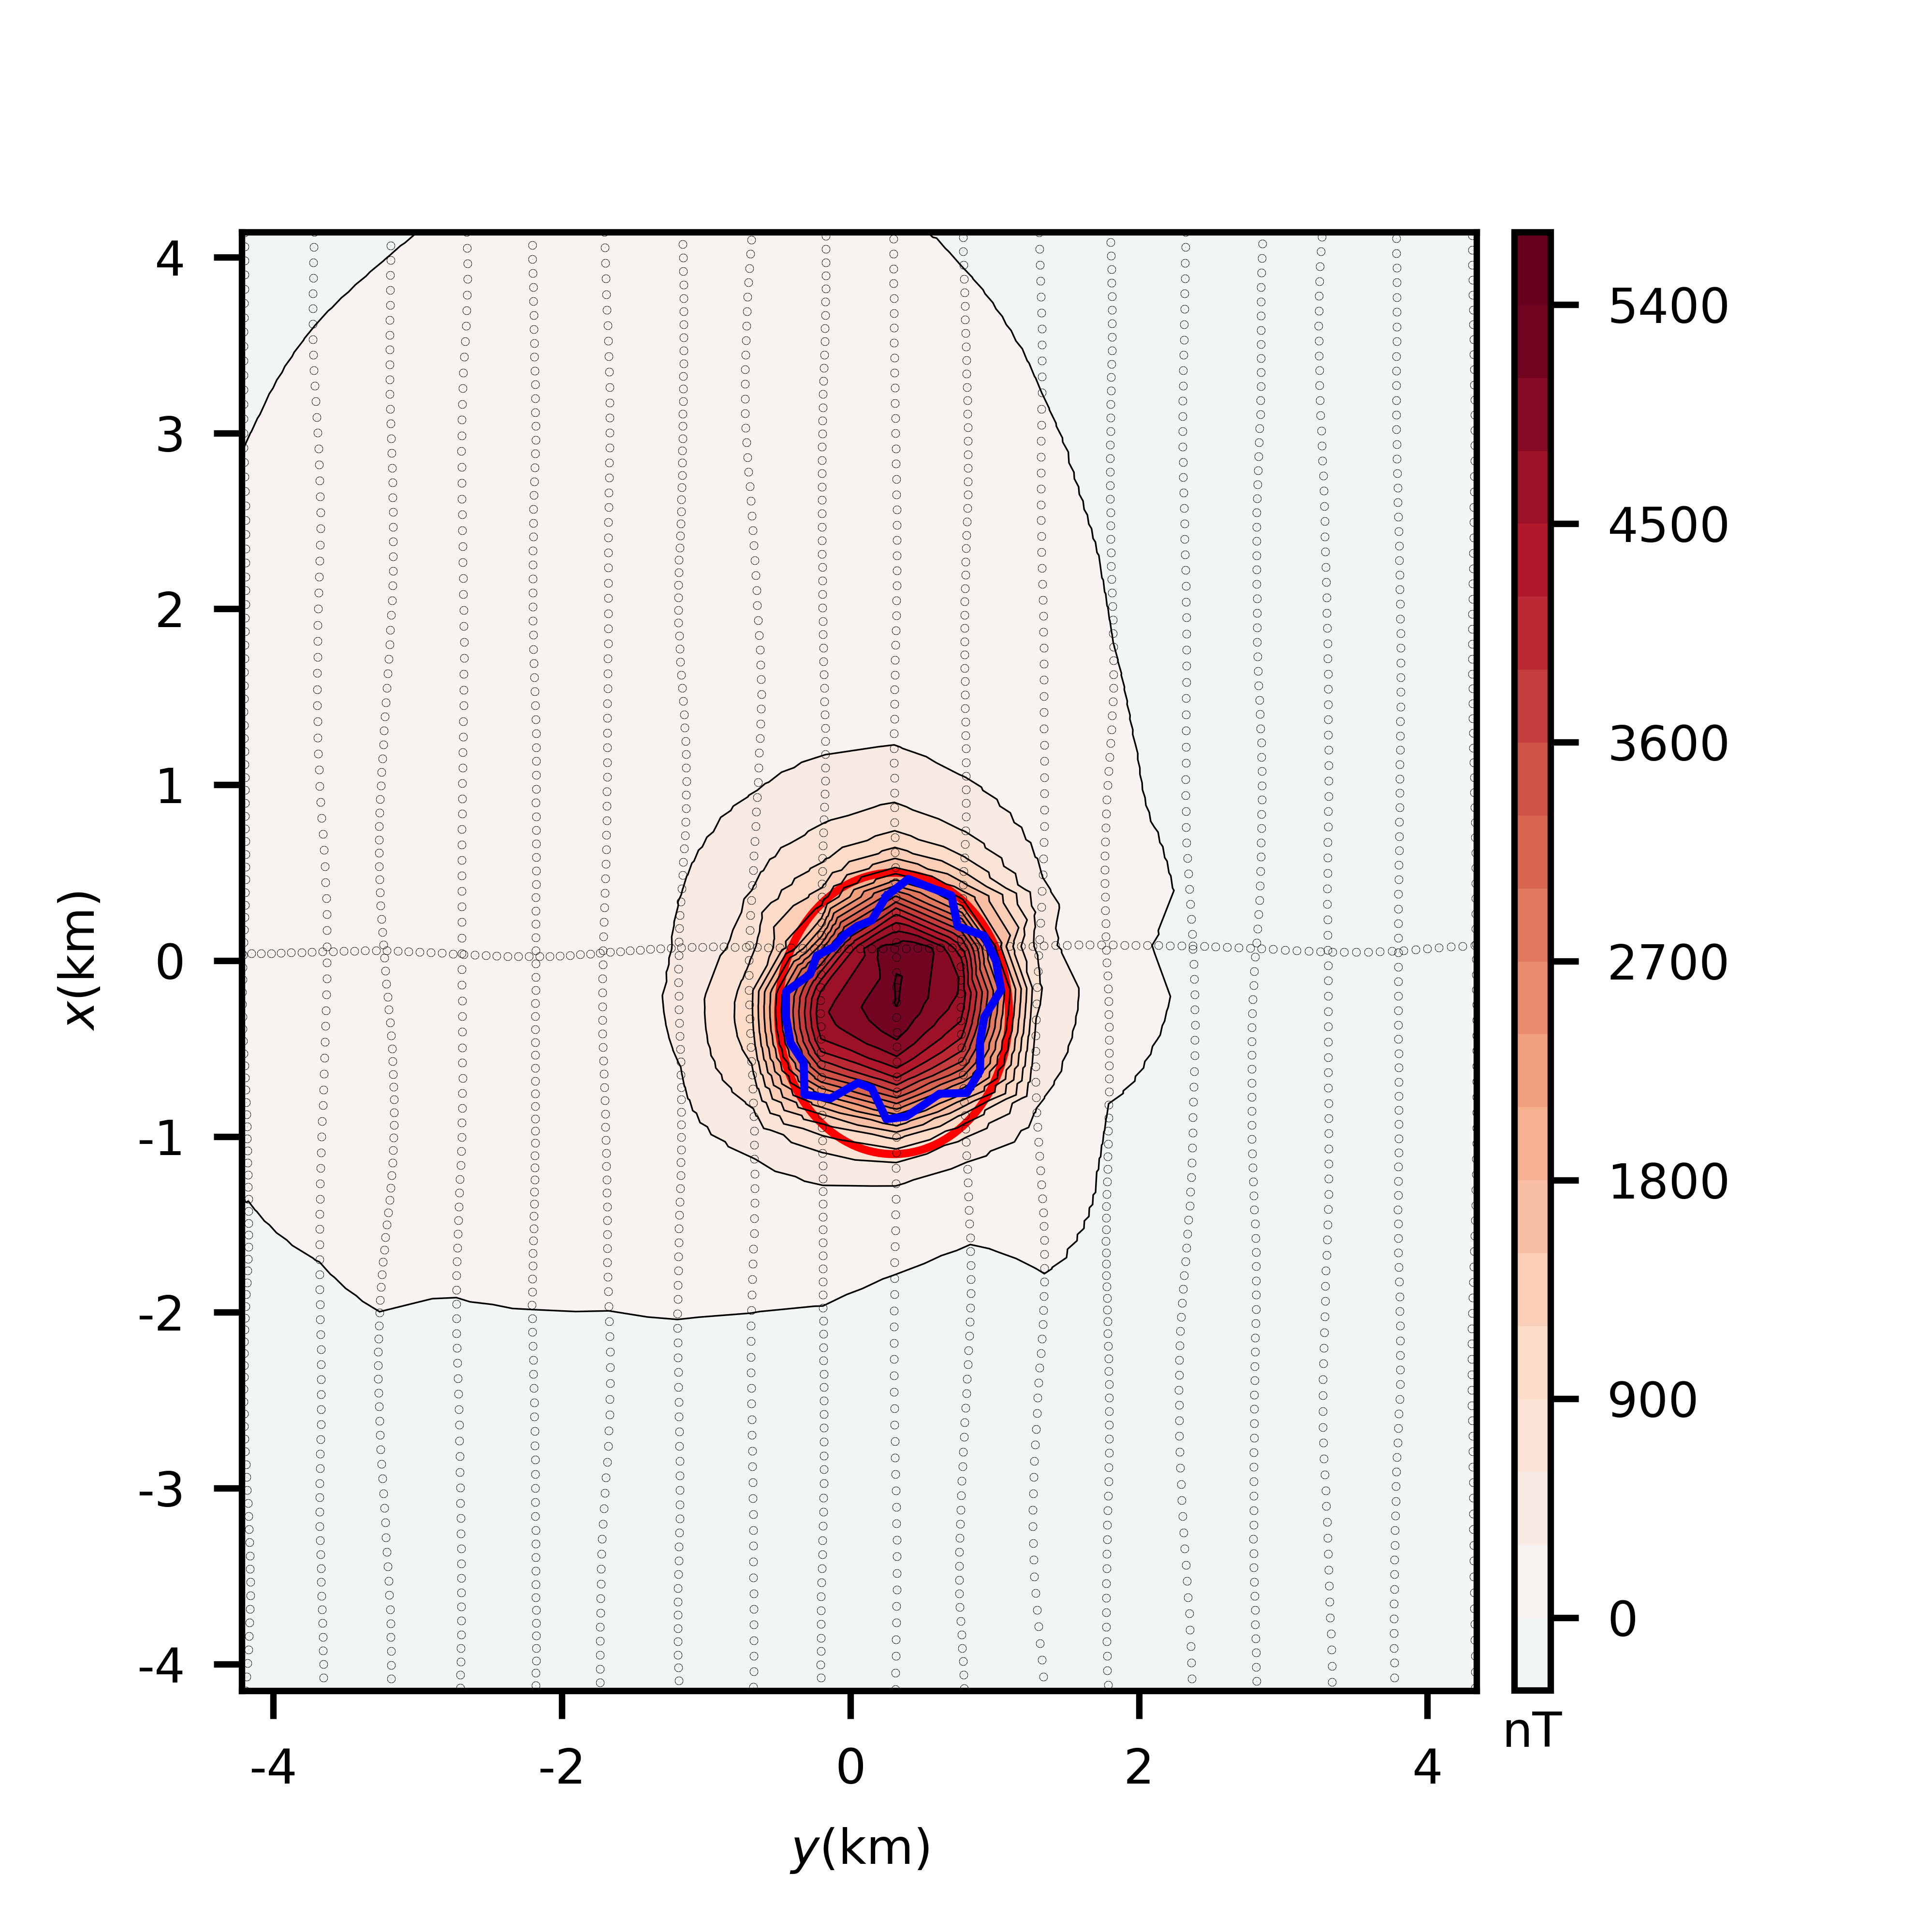
\includegraphics[width=\textwidth]{complex_rtp.png}
	\caption{Anomalia RTP produzida pela fonte alvo. 
		A anomalia RTP mostra valores predominantemente positivos logo acima da fonte alvo. Os pontos pretos representam os pontos de observação. As linhas azuis e vermelhas correspondem, respectivamente, às projeções horizontais da porção mais rasa da fonte alvo e da aproximação inicial utilizada nas inversões subsequentes (prismas vermelhos nas Figuras \ref{fig:target_l2_result}c e 
		\ref{fig:target_l1_result}c).
	}
	\label{fig:target_model_rtp}
\end{figure}

\pagebreak

\begin{figure}[!htb]
	\centering
	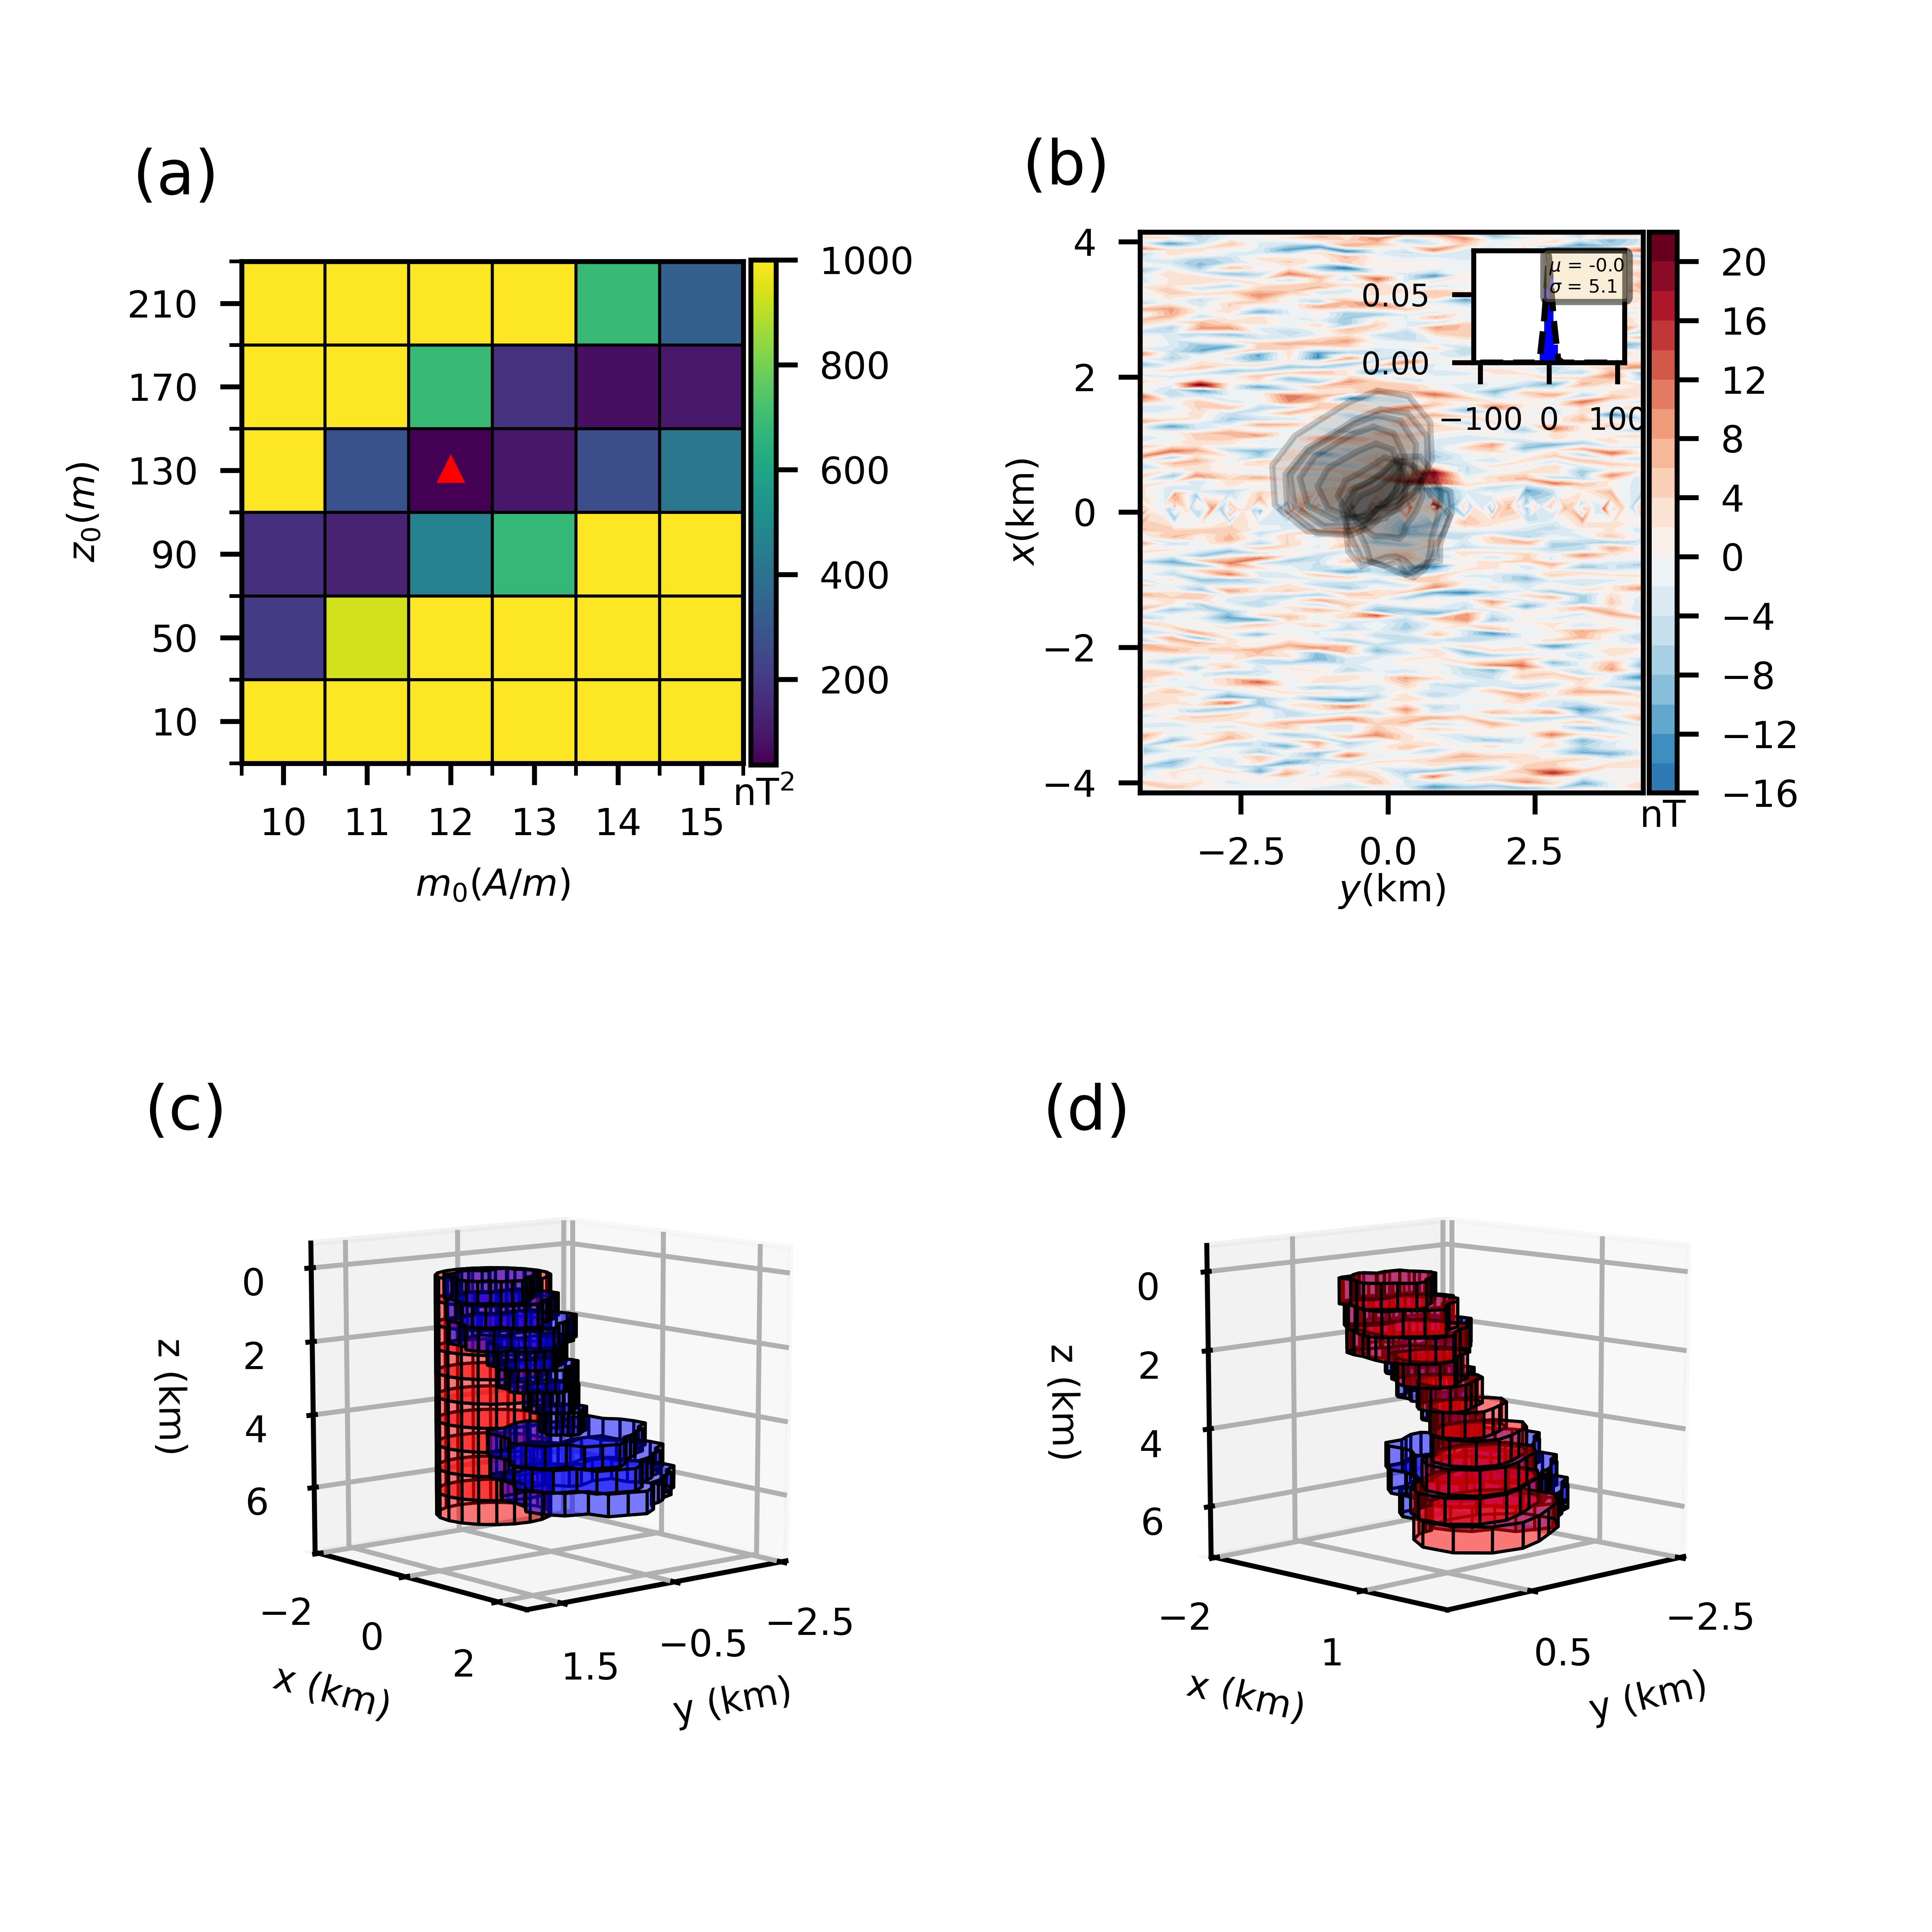
\includegraphics[width=\textwidth]{complex-l2-solution.png}
	\caption{Soluções L2 obtidas para o modelo da fonte alvo sem interferência. 
		(a) Mapa discreto da função objetivo produzida pelos modelos obtidos a partir da varredura de valores de profundidade do topo $z_{0}$ e intensidade de magnetização total $m_{0}$. 
		O triângulo vermelho representa os valores verdadeiros para $m_{0}$ e $z_{0}$, assim como os valores que definem a melhor solução L2.
		(b) Resíduos entre os dados contaminados com ruído (Figura \ref{fig:target_model}a) 
		e os dados preditos (não mostrados) produzidos pela melhor solução L2 (prismas vermelhos no painel d). 
		O histograma dos resíduos inserido em (b) mostra a curva Gaussiana ajustada (linha tracejada).
		Os polígonos cinzas representam as projeções horizontais de todos os prismas que compõe a melhor solução. 
		(c) e (d) Visualização em perspectiva da aproximação inicial (prismas vermelhos) e 
		a melhor solução (prismas vermelhos), respectivamente. Os prismas azuis são o modelo da fonte alvo. 
	}
	\label{fig:target_l2_result}
\end{figure}
\pagebreak
\begin{figure}[!htb]
	\centering
	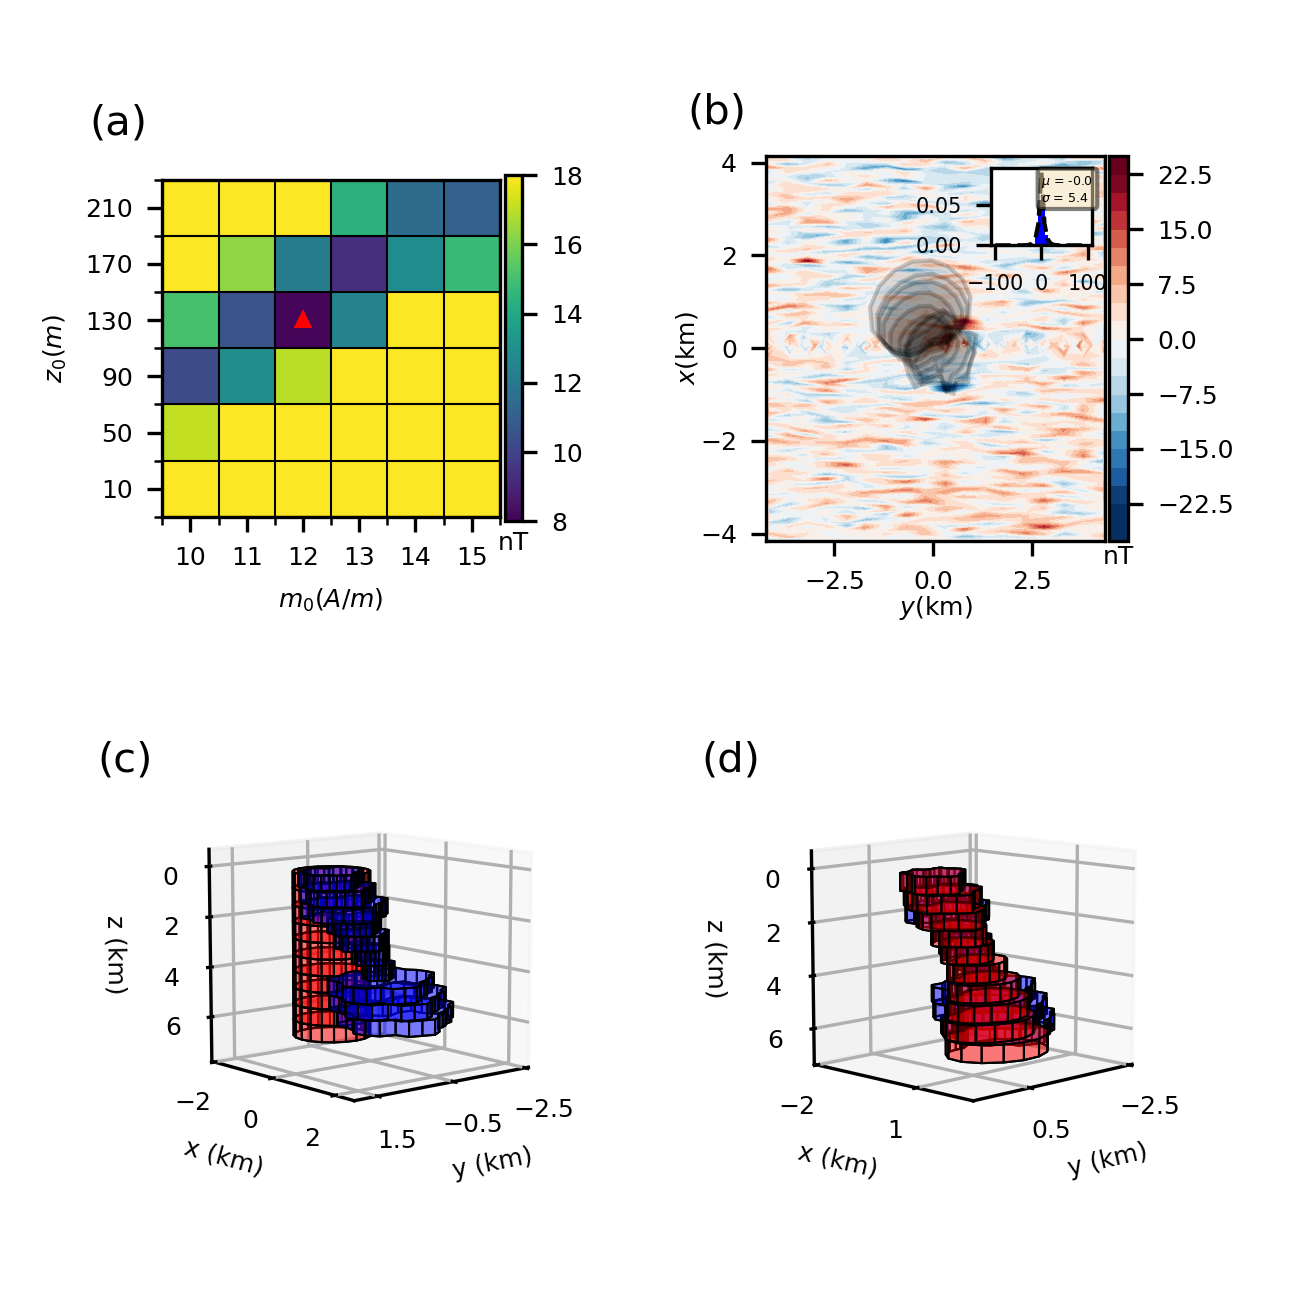
\includegraphics[width=\textwidth]{complex-l1-solution.png}
	\caption{Soluções L1 obtidas para o modelo da fonte alvo sem interferência. 
		(a) Mapa discreto da função objetivo produzida pelos modelos da malha de varredura para valores de profundidade do topo $z_{0}$ e intensidade de magnetização total $m_{0}$. 
		O triângulo vermelho representa os valores verdadeiros para $m_{0}$ e $z_{0}$, assim como os valores que definem a melhor solução L1.
		(b) Resíduos entre os dados contaminados com ruído (Figura \ref{fig:target_model}a) 
		e os dados preditos (não mostrados) produzidos pela melhor solução L1 (prismas vermelhos no painel d). 
		O histograma dos resíduos inserido em (b) mostra a curva Laplaciana ajustada (linha tracejada).
		Os polígonos cinzas representam as projeções horizontais de todos os prismas que compõe a melhor solução. 
		(c) e (d) Visualização em perspectiva da aproximação inicial (prismas vermelhos) e 
		a melhor solução (prismas vermelhos), respectivamente. Os prismas azuis são o modelo da fonte alvo. 
	}
	\label{fig:target_l1_result}
\end{figure}
\pagebreak


\section{Modelo complexo com uma fonte não-alvo pequena}
\label{sec:target_source_with_small_interference}


O mapa da Figura \ref{fig:small_model}a representa a soma entre as anomalias de campo total produzidas pela fonte não-alvo pequena (Figura \ref{fig:small_model}b), cuja forma é exibida nas Figuras \ref{fig:small_model}c e \ref{fig:small_model}d, e aquela produzida pela fonte alvo simulada (Figura \ref{fig:target_model}a). 
A fonte não-alvo possui profundidade do topo em $0$ m, profundidade da base em $70$ m, 
centro em $(x, y) = (-250, 250)$, logo acima da parte mais rasa da fonte alvo, e o mesmo vetor magnetização total da fonte alvo.
Embora a nova anomalia RTP produzida com a fonte não-alvo (Figura 
\ref{fig:small_model_rtp}) tenha uma amplitude maior que a produzida pela fonte alvo isolada (Figura \ref{fig:target_model_rtp}), a extensão horizontal da área positiva não muda substancialmente e conduz a uma aproximação inicial
(Figuras \ref{fig:small_l2_result}c e \ref{fig:small_l1_result}c) igual àquela utilizada no teste anterior (Figuras \ref{fig:target_l2_result}c e 
\ref{fig:target_l1_result}c).

A Figura \ref{fig:small_l2_result} mostra as soluções L2 obtidas pela inversão da anomalia de campo total na Figura \ref{fig:small_model}a
com os seguintes pesos normalizados $\tilde{\alpha}_{\ell}$ (Equação \ref{eq:alphas}):
$\tilde{\alpha}_{1} = 10^{-5}$, $\tilde{\alpha}_{2} = 10^{-4}$, 
$\tilde{\alpha}_{3} = 10^{-4}$, $\tilde{\alpha}_{4} = 10^{-8}$, e 
$\tilde{\alpha}_{5} = 10^{-5}$.
A Figura \ref{fig:small_l2_result}a mostra que a melhor solução L2 possui profundidade do topo $z_{0}$ igual à verdadeira, porém possui uma intensidade de magnetização total $m_{0}$ superestimada. Por esse motivo, sua profundidade máxima 
($3046.8$ m) é muito distante da verdadeira ($6130$ m).
Essa solução produz valores de resíduos altos logo acima da fonte não-alvo 
(Figura \ref{fig:small_l2_result}b), mas esses resíduos diferem consideravelmente da anomalia de campo total produzida pela fonte não-alvo (Figura \ref{fig:small_model}b).
Isso significa que, nesse caso, a inversão não foi capaz de ignorar o efeito causado pela fonte não-alvo.
Além disso, a Figura \ref{fig:small_l2_result}d mostra que a melhor solução L2 não recupera a forma da fonte alvo.

A Figura \ref{fig:small_l1_result} mostra as soluções L1 obtidas pela inversão da anomalia de campo total exibida na Figura \ref{fig:small_model}a
com os mesmos pesos normalizados $\tilde{\alpha}_{\ell}$ (Equação \ref{eq:alphas})
utilizados para as soluções L2 (Figura \ref{fig:small_l2_result}).
Comparada à solução L2 mostrada na Figura \ref{fig:small_l2_result}, a melhor solução L1 apresenta uma intensidade de magnetização total menos superestimada (Figura 
\ref{fig:small_l1_result}a) e profundidade da base ($5176.4$ m) menos subestimada cerca de $ 1 $ km de diferença em relação à verdadeira ($6130$ m). Essa solução produz valores de resíduos (Figura \ref{fig:small_l1_result}b) 
próximos à anomalia de campo total produzida pela fonte não-alvo (Figura 
\ref{fig:small_model}b). 
Isso significa que, nesse caso, a performance do método foi mais eficaz em filtrar a anomalia de campo total não-alvo (Figura \ref{fig:small_model}b).
Como consequência, a solução L1 (Figura \ref{fig:small_l1_result}d) foi muito menos afetada pela fonte não-alvo e recuperou satisfatoriamente a forma da fonte alvo. 
Este teste numérico mostra que a solução L1 é superior à solução L2 mesmo que a fonte não-alvo seja muito localizada e menor do que a fonte alvo.
\pagebreak
\begin{figure}[!htb]
	\centering
	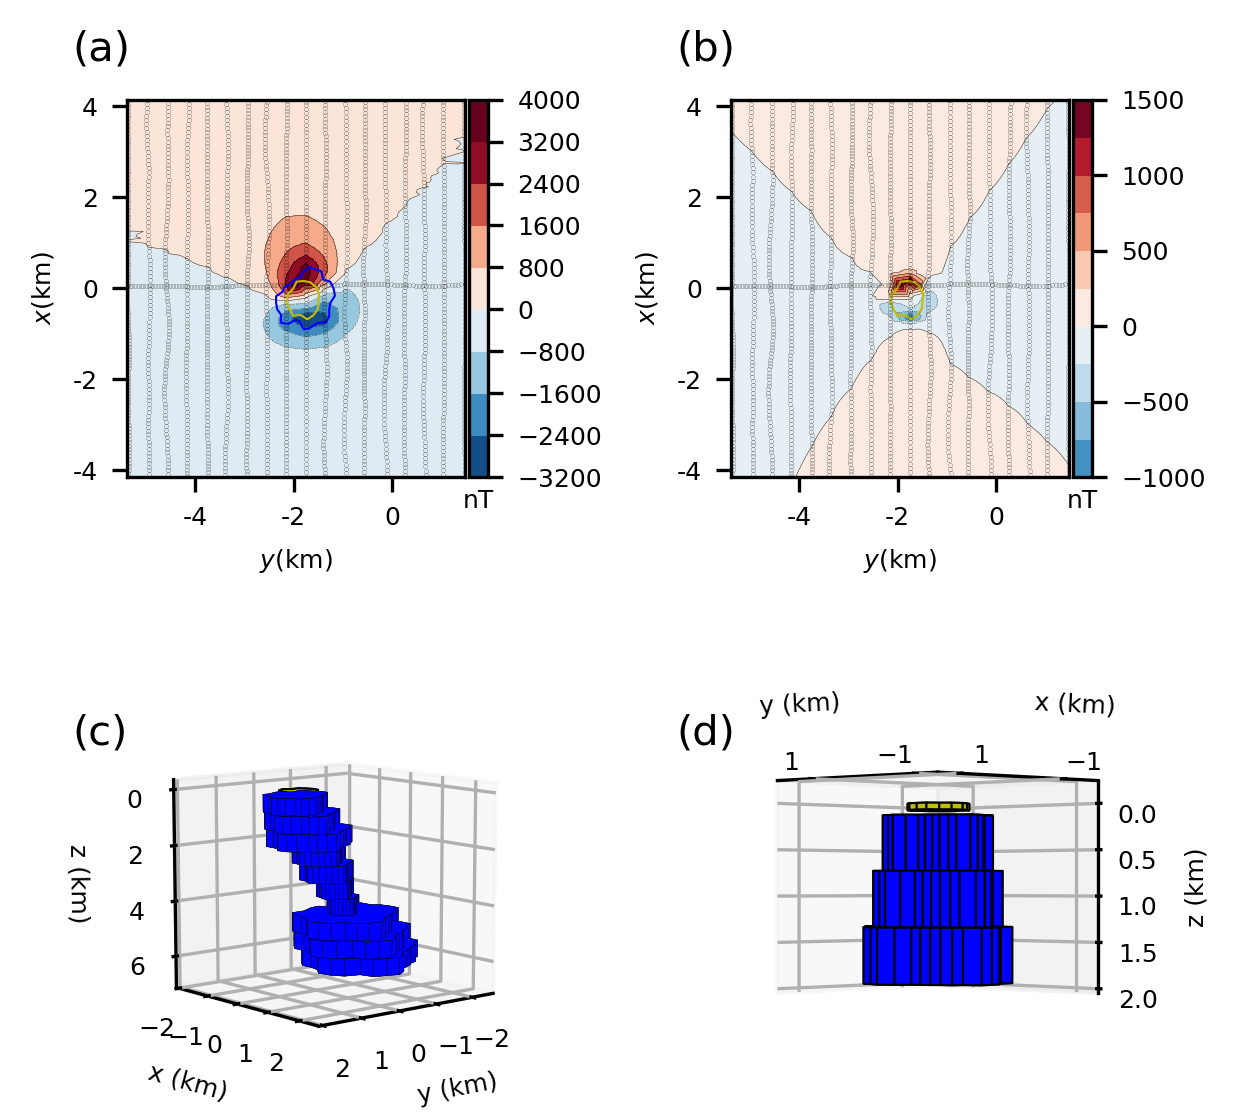
\includegraphics[width=\textwidth]{small_model_data.png}
	\caption{Modelo da fonte alvo com uma fonte não-alvo pequena.
		(a) Anomalia de campo total produzida pelas fontes alvo e não-alvo
		(prismas azuis e amarelos nos painéis c e d). Os pontos pretos representam os pontos de observação. Os polígonos azul e amarelo são as projeções horizontais das fontes alvo e não-alvo, respectivamente.
		(b) A anomalia de campo total produzida pela fonte não-alvo. 
		(c) Visualização em perspectiva da fonte alvo (prismas azuis) e da fonte não-alvo (prisma amarelo). 
		(d) Visualização em perspectiva aproximada das fontes alvo (prismas azuis) e não-alvo (prisma amarelo).
	}
	\label{fig:small_model}
\end{figure}
\pagebreak
\begin{figure}[!htb]
	\centering
	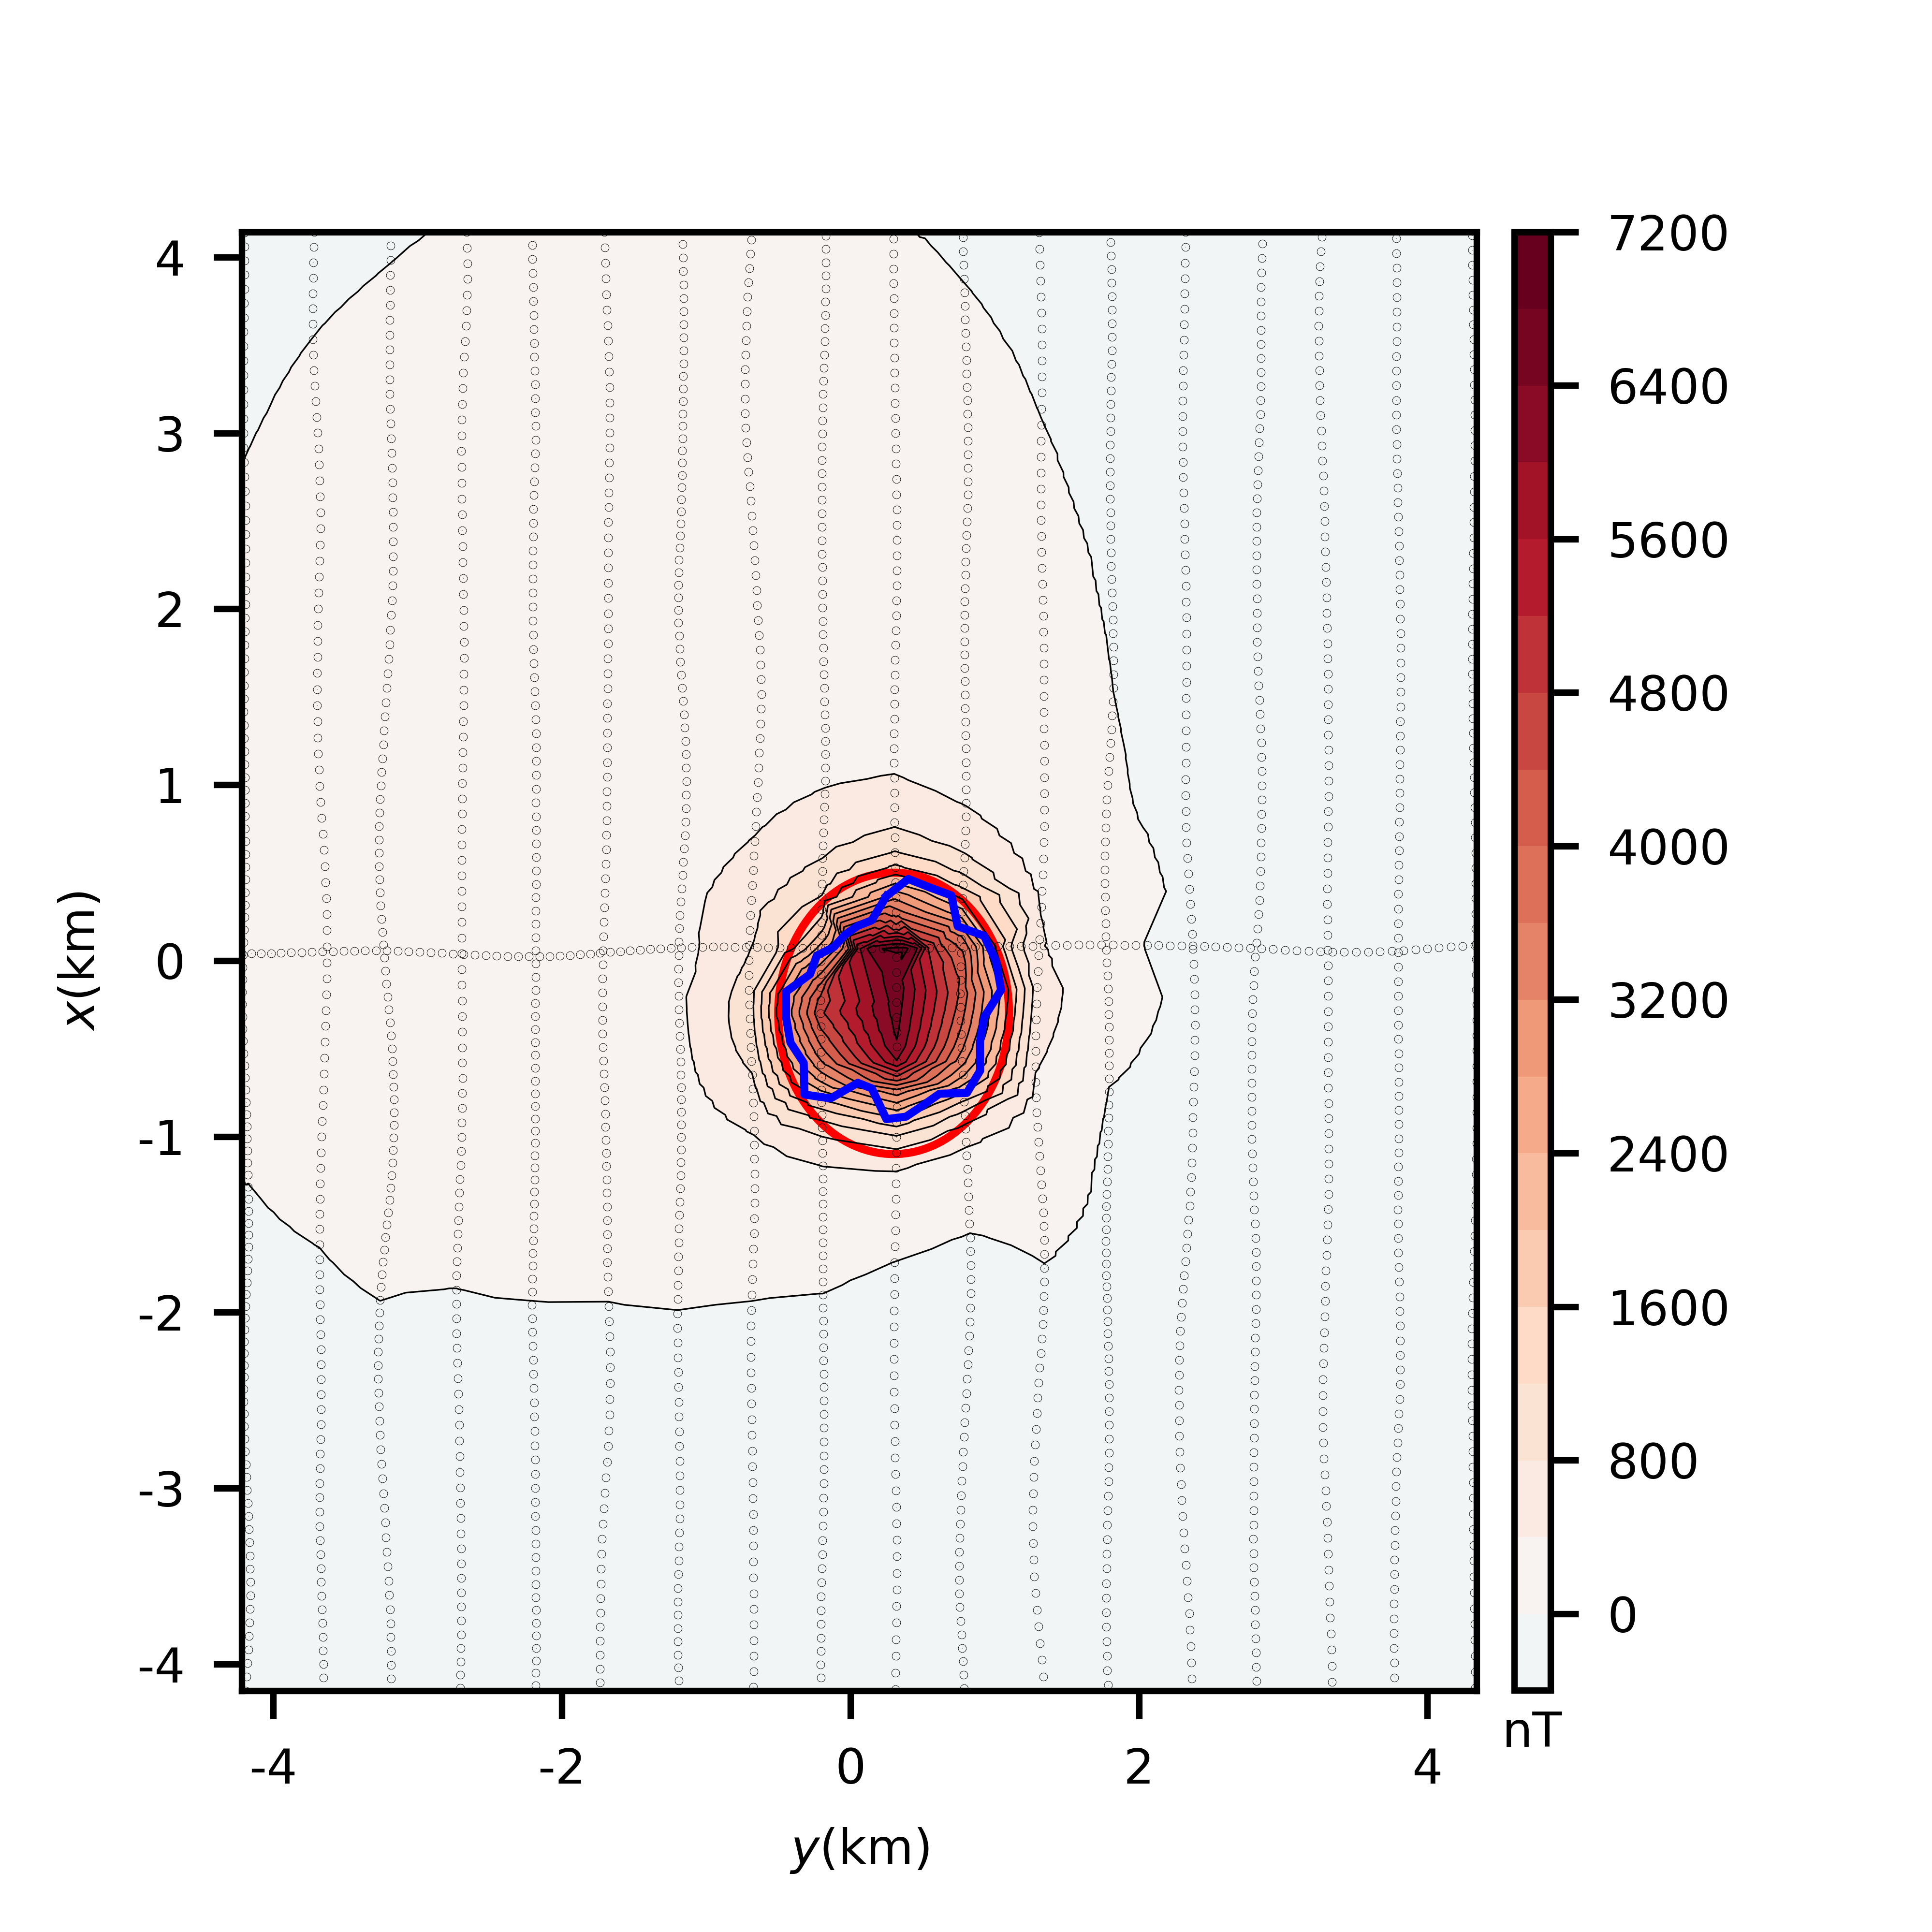
\includegraphics[width=\textwidth]{small_rtp.png}
	\caption{Anomalia RTP estimada produzida pela fonte alvo com uma fonte não-alvo pequena. 
		A anomalia RTP mostra valores predominantemente positivos logo acima da fonte alvo. Os pontos pretos representam os pontos de observação. As linhas azuis e vermelhas correspondem, respectivamente, às projeções horizontais da porção mais rasa da fonte alvo e da aproximação inicial utilizada nas inversões subsequentes (prismas vermelhos nas Figuras \ref{fig:small_l2_result}c e 
		\ref{fig:small_l1_result}c).
	}
	\label{fig:small_model_rtp}
\end{figure}
\pagebreak
\begin{figure}[!htb]
	\centering
	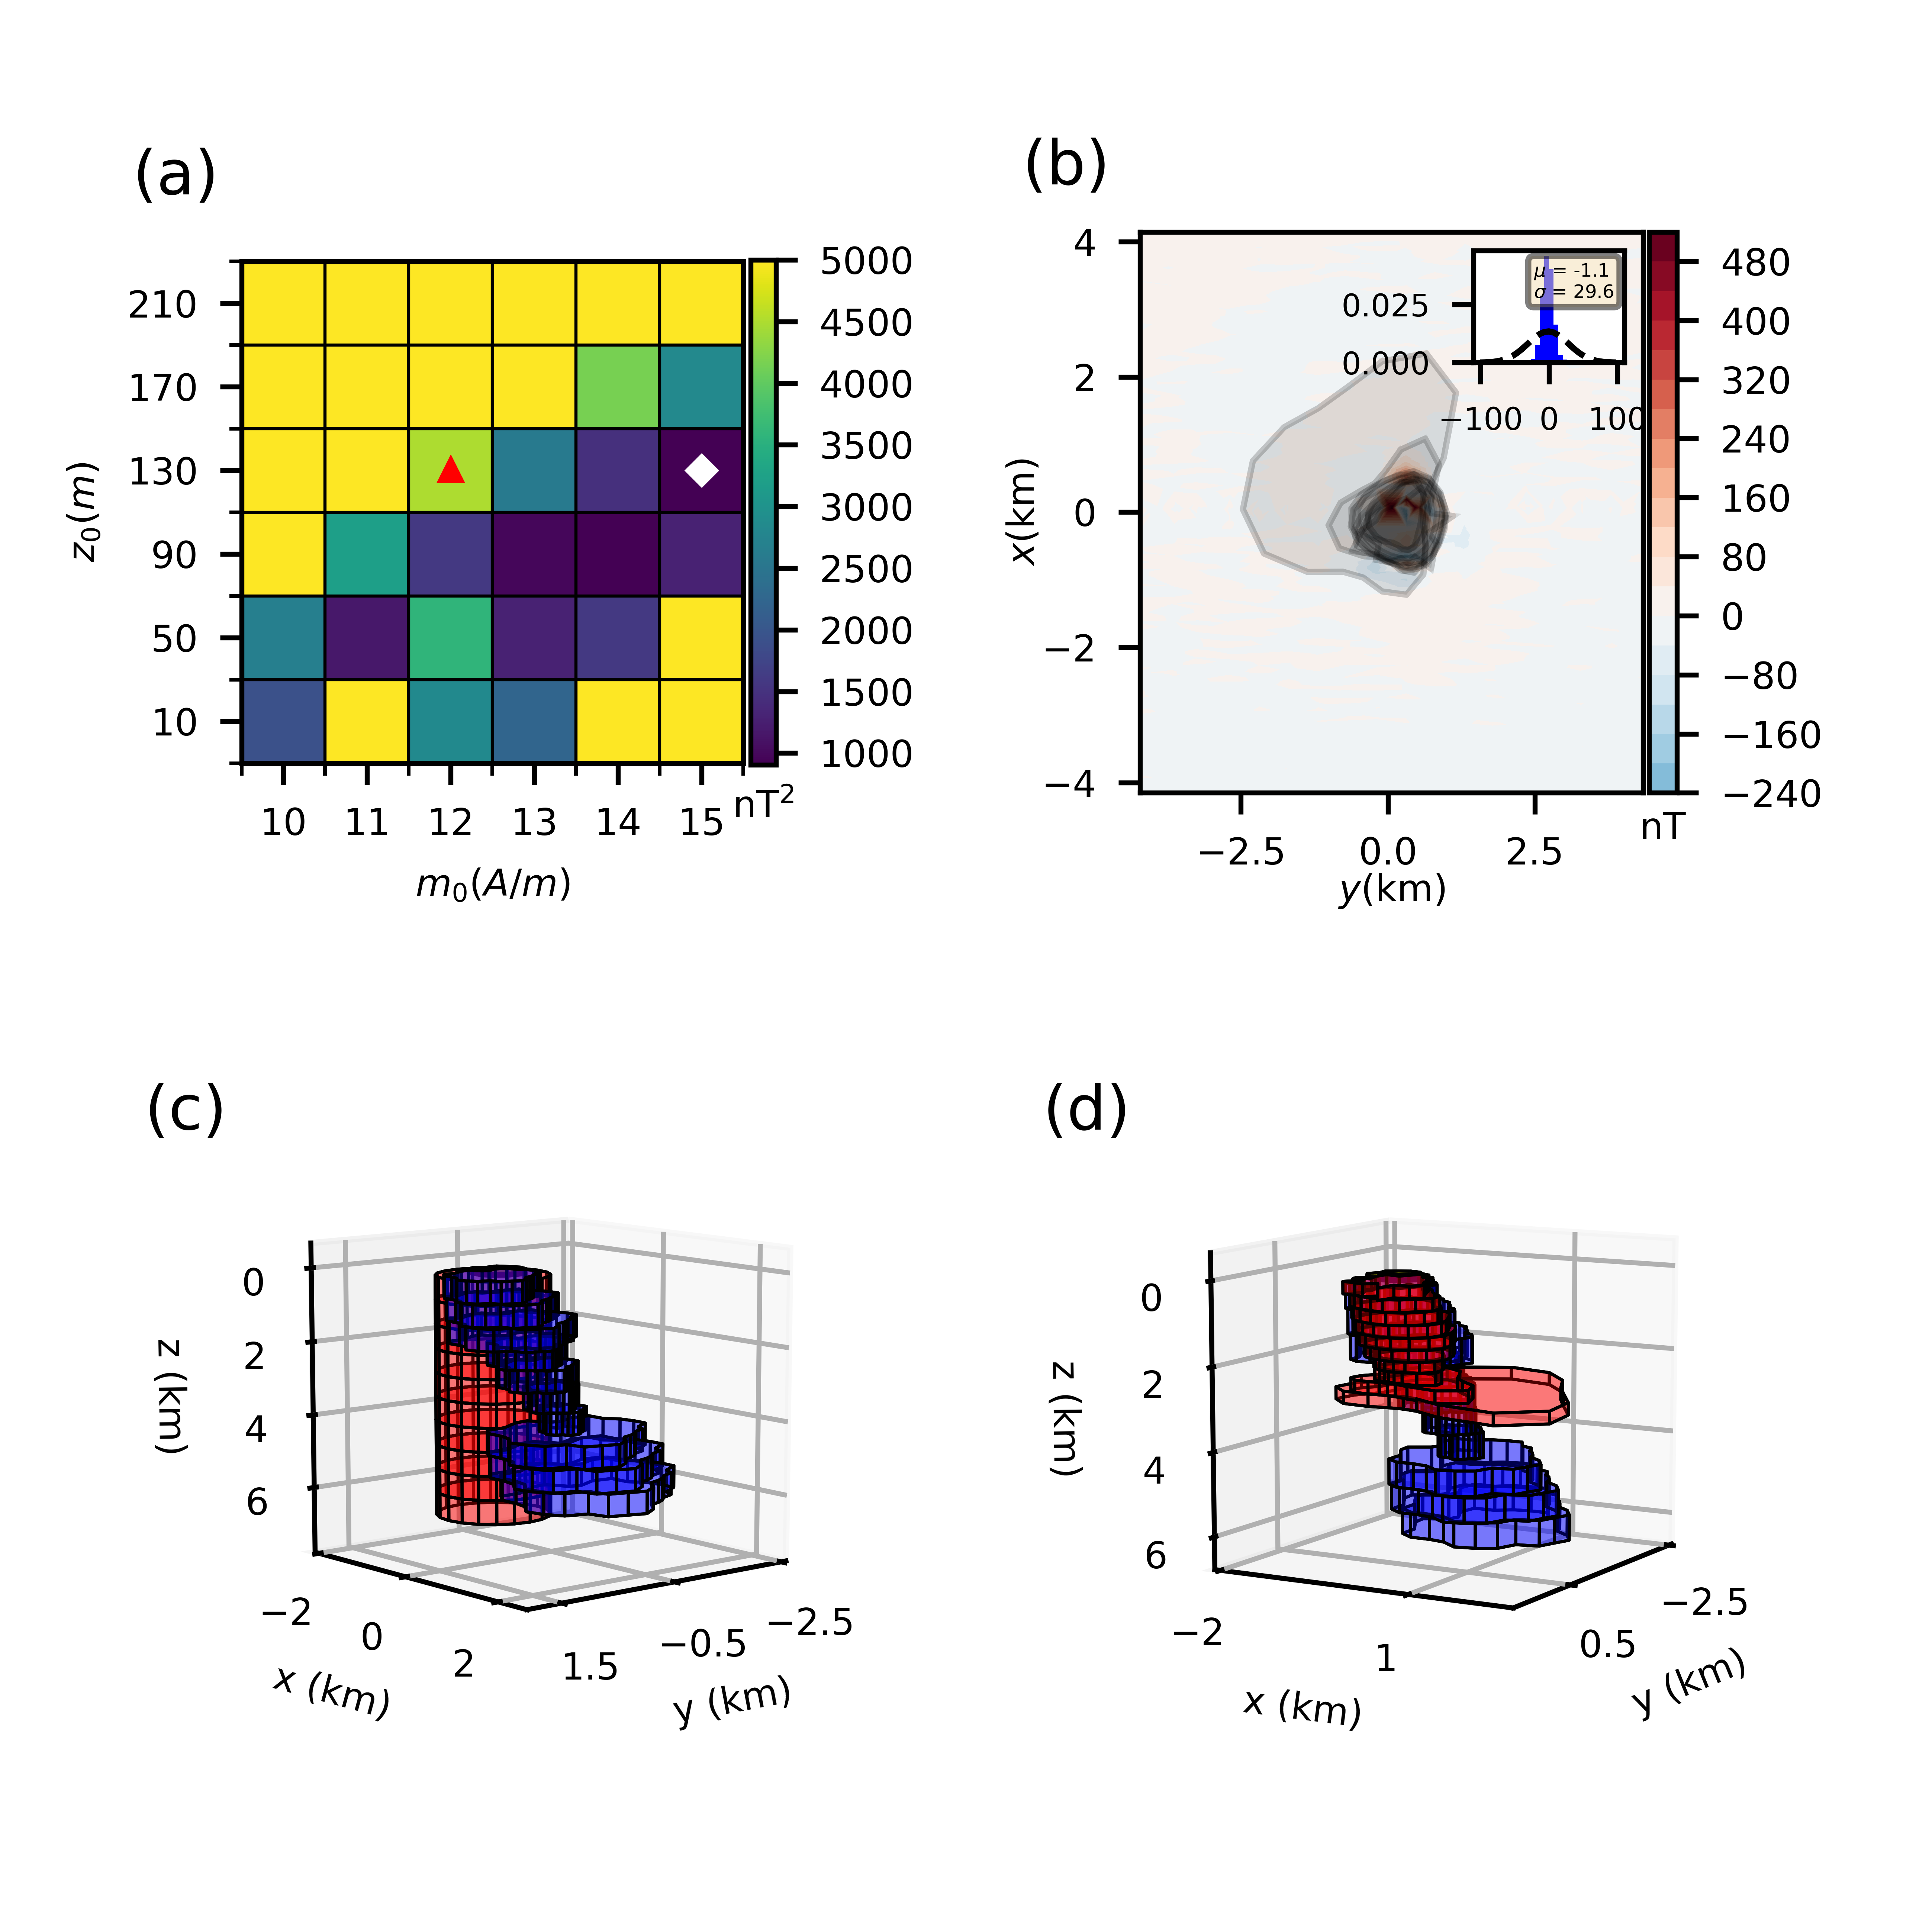
\includegraphics[width=\textwidth]{small-l2-solution.png}
	\caption{Soluções L2 obtidas para o modelo da fonte alvo com uma fonte não-alvo pequena. 
		(a) Mapa discreto da função objetivo produzida pelos modelos da malha de varredura para valores de profundidade do topo $z_{0}$ e intensidade de magnetização total $m_{0}$. 
		Os valores verdadeiros de $m_{0}$ e $z_{0})$ e aqueles que definem a melhor solução L2 são representados pelo triângulo vermelho e pelo losango branco, respectivamente.
		(b) Resíduos entre os dados contaminados com ruído (Figura \ref{fig:target_model}a) 
		e os dados preditos (não mostrados) produzidos pela melhor solução L2 (prismas vermelhos no painel d). 
		O histograma dos resíduos inserido em (b) mostra a curva Gaussiana ajustada (linha tracejada).
		Os polígonos cinzas representam as projeções horizontais de todos os prismas que compõe a melhor solução. 
		(c) e (d) Visualização em perspectiva da aproximação inicial (prismas vermelhos) e 
		a melhor solução (prismas vermelhos), respectivamente. Os prismas azuis são o modelo da fonte alvo.
	}
	\label{fig:small_l2_result}
\end{figure}
\pagebreak
\begin{figure}[!htb]
	\centering
	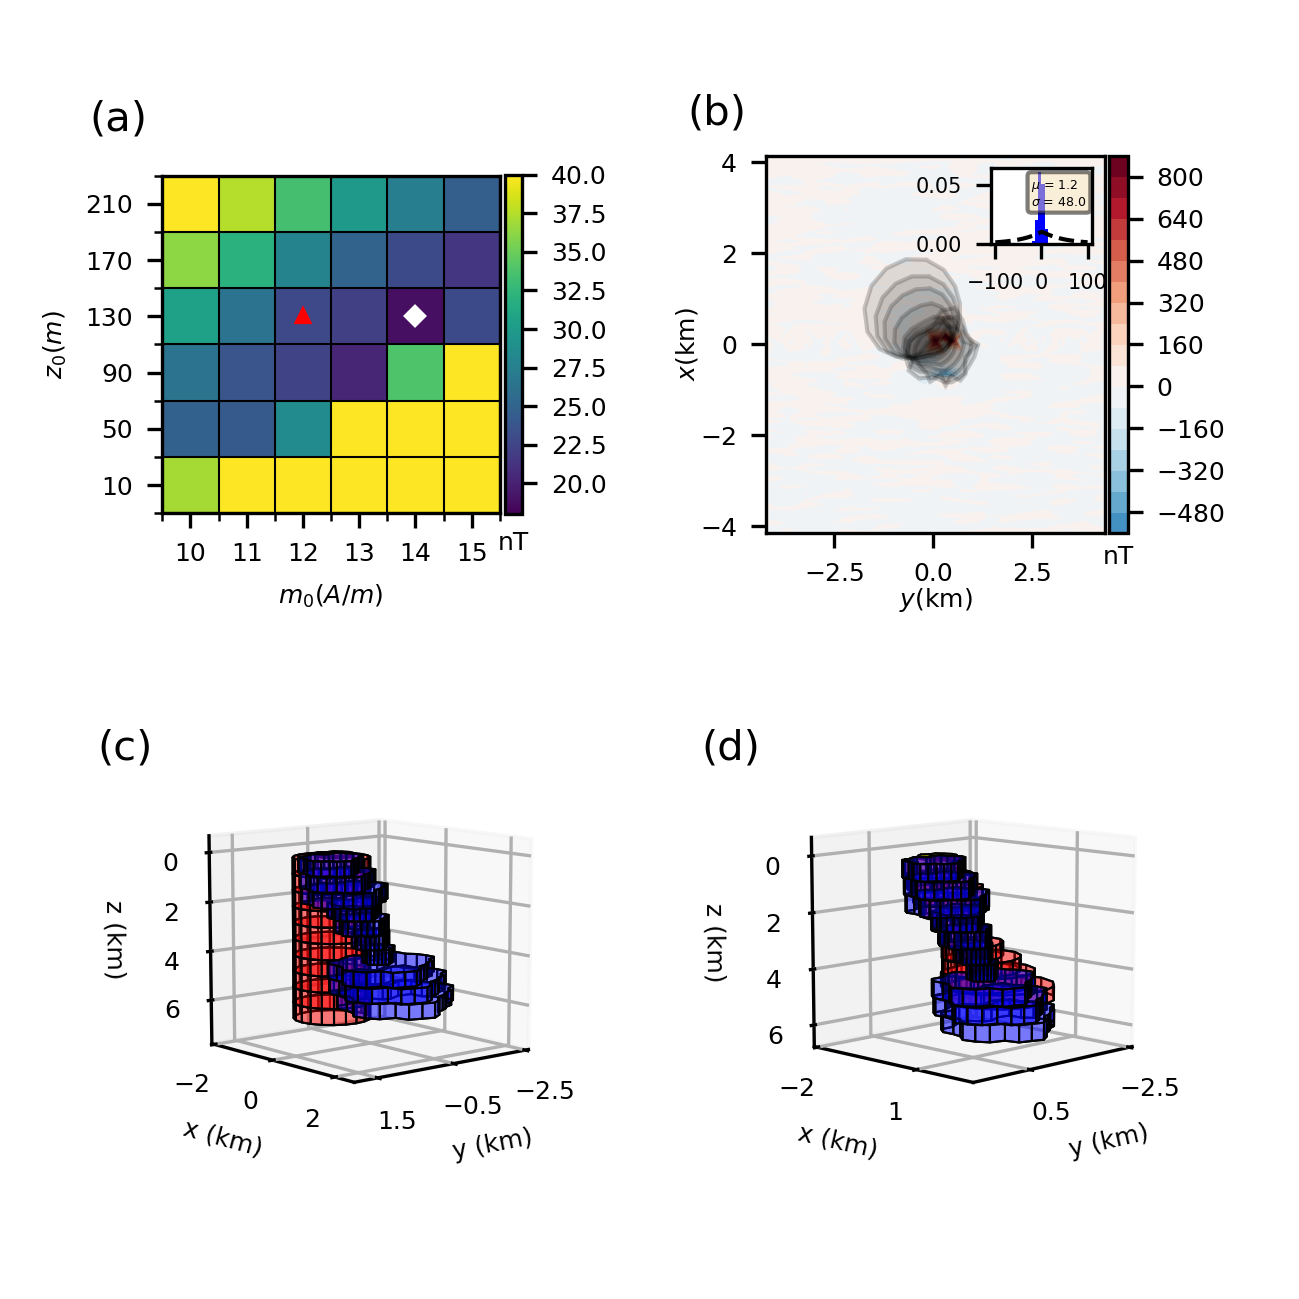
\includegraphics[width=\textwidth]{small-l1-solution.png}
	\caption{Soluções L1 obtidas para o modelo da fonte alvo com uma fonte não-alvo pequena. 
		(a) Mapa discreto da função objetivo produzida pelos modelos da malha de varredura para valores de profundidade do topo $z_{0}$ e intensidade de magnetização total $m_{0}$. 
		Os valores verdadeiros de $m_{0}$ e $z_{0})$ e aqueles que definem a melhor solução L1 são representados pelo triângulo vermelho e pelo losango branco, respectivamente.
		(b) Resíduos entre os dados contaminados com ruído (Figura \ref{fig:target_model}a) 
		e os dados preditos (não mostrados) produzidos pela melhor solução L1 (prismas vermelhos no painel d). 
		O histograma dos resíduos inserido em (b) mostra a curva Gaussiana ajustada (linha tracejada).
		Os polígonos cinzas representam as projeções horizontais de todos os prismas que compõe a melhor solução. 
		(c) e (d) Visualização em perspectiva da aproximação inicial (prismas vermelhos) e 
		a melhor solução (prismas vermelhos), respectivamente. Os prismas azuis são o modelo da fonte alvo. 
	}
	\label{fig:small_l1_result}
\end{figure}
\pagebreak
\section{Modelo complexo com uma fonte não-alvo grande}
\label{sec:target_source_with_large_interference}

O mapa da Figura \ref{fig:thick_model}a representa a soma entre as anomalias de campo total produzidas pela fonte não-alvo pequena (Figura \ref{fig:thick_model}b), cuja forma é exibida nas Figuras \ref{fig:thick_model}c e \ref{fig:thick_model}d, e aquela produzida pela fonte alvo simulada (Figura \ref{fig:target_model}a).
A fonte não-alvo possui profundidade do topo em $0$ m, profundidade da base em $500$ m, 
centro em $(x, y) = (500, 1500)$, ao lado do topo da fonte alvo, e o mesmo vetor magnetização total da fonte alvo.
Neste caso, a fonte não-alvo estende consideravelmente a área positiva da anomalia RTP (Figura \ref{fig:thick_model_rtp}) em comparação com a da fonte alvo isolada (Figura \ref{fig:target_model_rtp}). Entretanto, ainda é possível identificar os limites laterais da fonte alvo e gerar a mesma aproximação inicial usada nos testes anteriores.


A Figura \ref{fig:thick_l2_result} mostra as soluções L2 obtidas pela inversão da anomalia de campo total na Figura \ref{fig:thick_model}a
com os seguintes pesos normalizados $\tilde{\alpha}_{\ell}$ (Equação \ref{eq:alphas}):
$\tilde{\alpha}_{1} = 10^{-4}$, $\tilde{\alpha}_{2} = 10^{-5}$, 
$\tilde{\alpha}_{3} = 10^{-4}$, $\tilde{\alpha}_{4} = 10^{-7}$, e 
$\tilde{\alpha}_{5} = 10^{-7}$.
Como podemos ver, a melhor solução L2 não recupera os valores da profundidade do topo $z_{0}$ e nem da intensidade de magnetização total $m_{0}$, assim como não recuperou a forma da fonte alvo.
A estimativa da profundidade da base ($2010.1$ m) é muito distante da verdadeira ($6130$ m).
Comparado ao valor verdadeiro, a profundidade do topo estimada $z_{0}$ está deslocada em direção à da fonte não-alvo.
Nesse caso, a fonte não-alvo induz severamente ao erro da estimativa da geometria do corpo (Figura \ref{fig:thick_l2_result}d).

A Figura \ref{fig:thick_l1_result} mostra as soluções L1 obtidas pela inversão da anomalia de campo total mostrada na Figura \ref{fig:thick_model}a
com os seguintes pesos normalizados $\tilde{\alpha}_{\ell}$ (Equação \ref{eq:alphas}):
$\tilde{\alpha}_{1} = 10^{-4}$, $\tilde{\alpha}_{2} = 10^{-5}$, 
$\tilde{\alpha}_{3} = 10^{-4}$, $\tilde{\alpha}_{4} = 10^{-7}$, e 
$\tilde{\alpha}_{5} = 10^{-7}$.
A melhor solução L1 (Figura \ref{fig:thick_l1_result}) filtra parcialmente a anomalia de campo total não-alvo (Figura \ref{fig:thick_model}b) e recupera as principais feições da fonte alvo sintética, assim como a profundidade do topo $z_{0}$ e a intensidade de magnetização total $m_{0}$ verdadeiras.
Essa solução estima a profundidade da base ($5840.9$ m) melhor do que a do teste anterior, no entanto, a solução é inferior à mostrada no teste anterior em filtrar a anomalia de campo total não-alvo e também em recuperar a geometria da fonte alvo.
Apesar disso, ela é significativamente superior à melhor solução L2 (Figura \ref{fig:thick_l2_result}) obtida pela inversão do mesmo dado, uma vez que é muito menos afetada pela presença de uma grande fonte não-alvo.
\pagebreak
\begin{figure}[!htb]
	\centering
	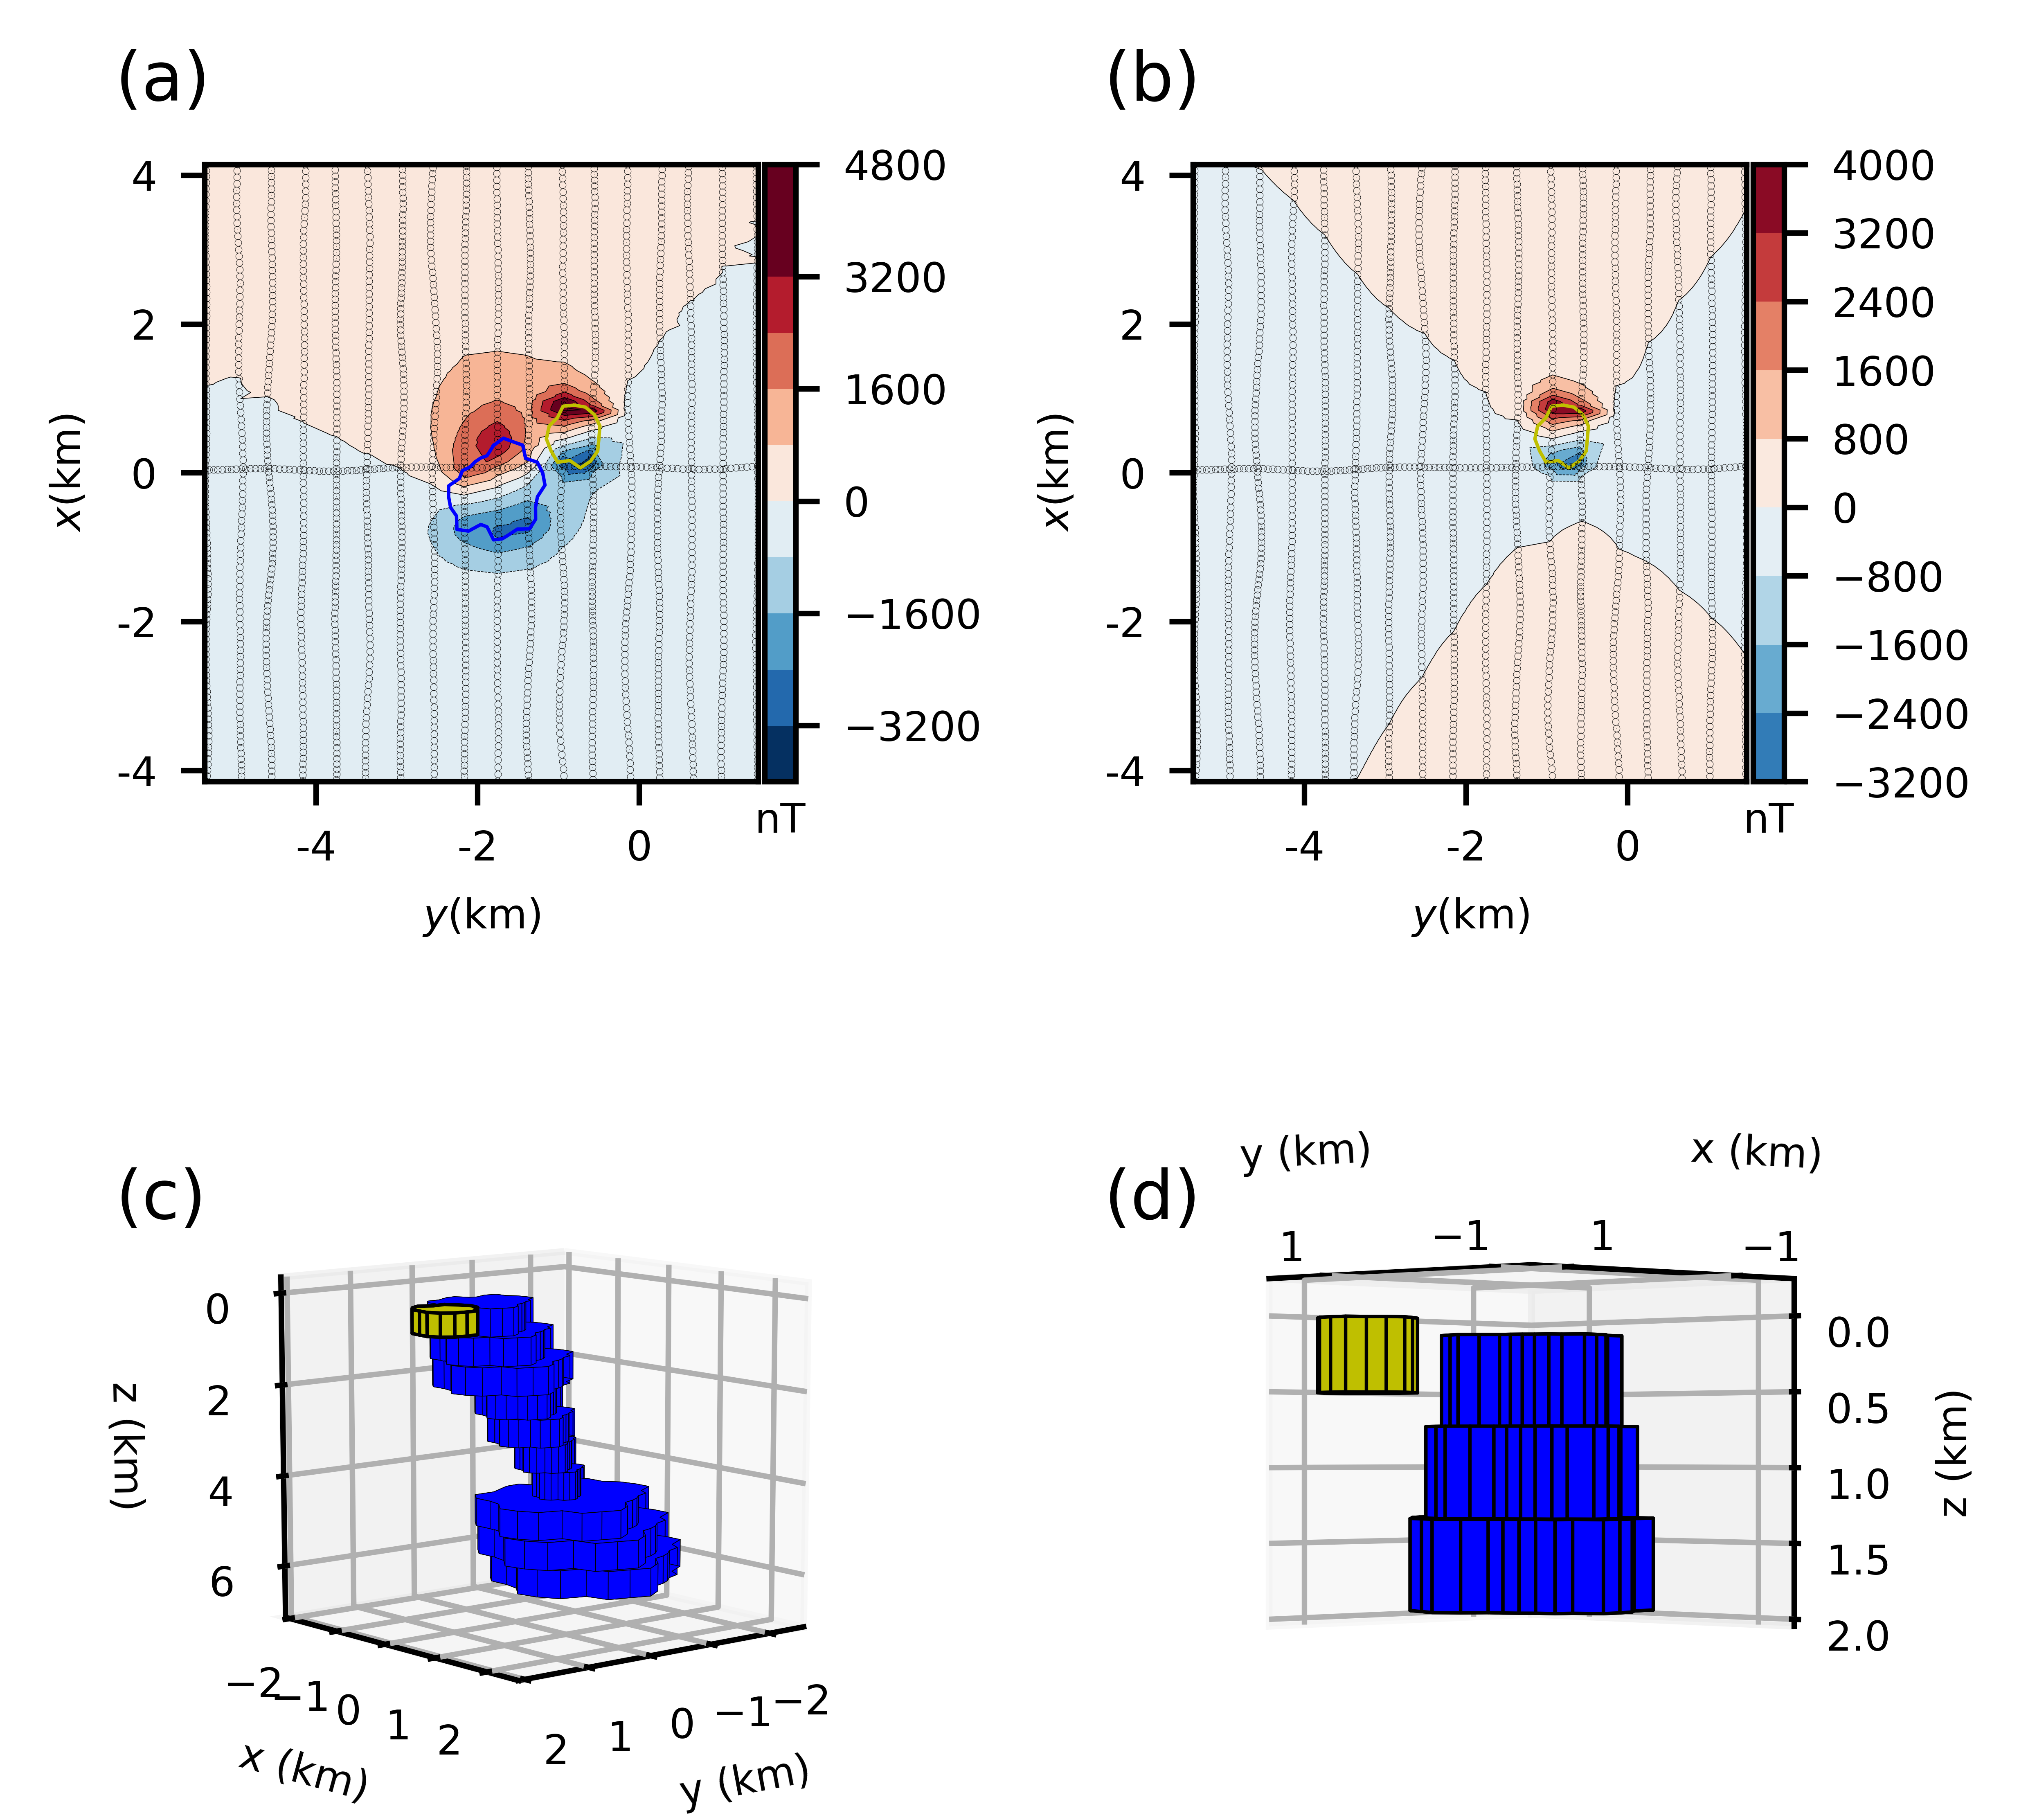
\includegraphics[width=\textwidth]{thick_model_data.png}
	\caption{Modelo da fonte alvo com uma fonte não-alvo grande.
		(a) Anomalia de campo total produzida pelas fontes alvo e não-alvo
		(prismas azuis e amarelos nos painéis c e d). Os pontos pretos representam os pontos de observação. Os polígonos azul e amarelo são as projeções horizontais das fontes alvo e não-alvo, respectivamente.
		(b) A anomalia de campo total produzida pela fonte não-alvo. 
		(c) Visualização em perspectiva da fonte alvo (prismas azuis) e da fonte não-alvo (prisma amarelo). 
		(d) Visualização em perspectiva aproximada das fontes alvo (prismas azuis) e não-alvo (prisma amarelo).
	}
	\label{fig:thick_model}
\end{figure}
\pagebreak

\begin{figure}[!htb]
	\centering
	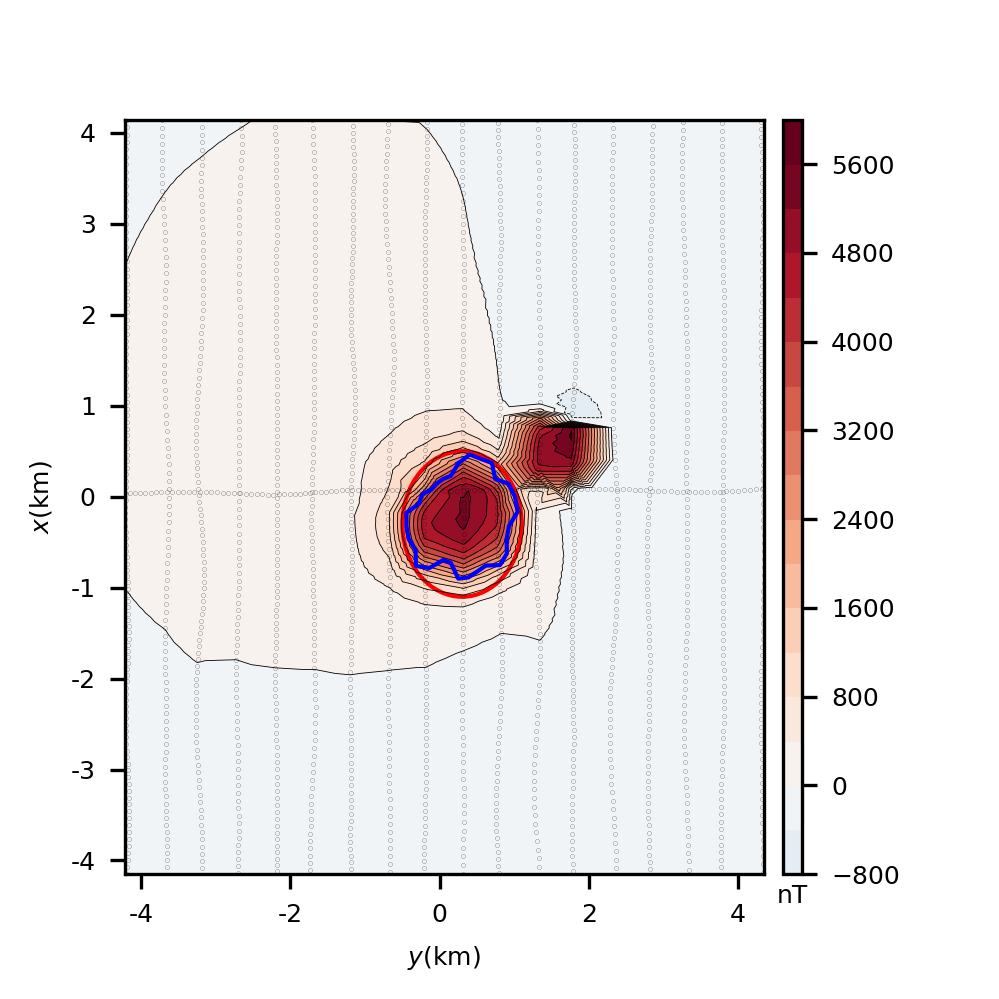
\includegraphics[width=\textwidth]{thick_rtp.png}
	\caption{Anomalia RTP estimada produzida pela fonte alvo com uma fonte não-alvo grande. 
		A anomalia RTP mostra valores predominantemente positivos logo acima das fontes alvo e não-alvo. Os pontos pretos representam os pontos de observação. As linhas azuis e vermelhas correspondem, respectivamente, às projeções horizontais da porção mais rasa da fonte alvo e da aproximação inicial utilizada nas inversões subsequentes (prismas vermelhos nas Figuras \ref{fig:thick_l2_result}c e 
		\ref{fig:thick_l1_result}c).
	}
	\label{fig:thick_model_rtp}
\end{figure}
\pagebreak
\begin{figure}[!htb]
	\centering
	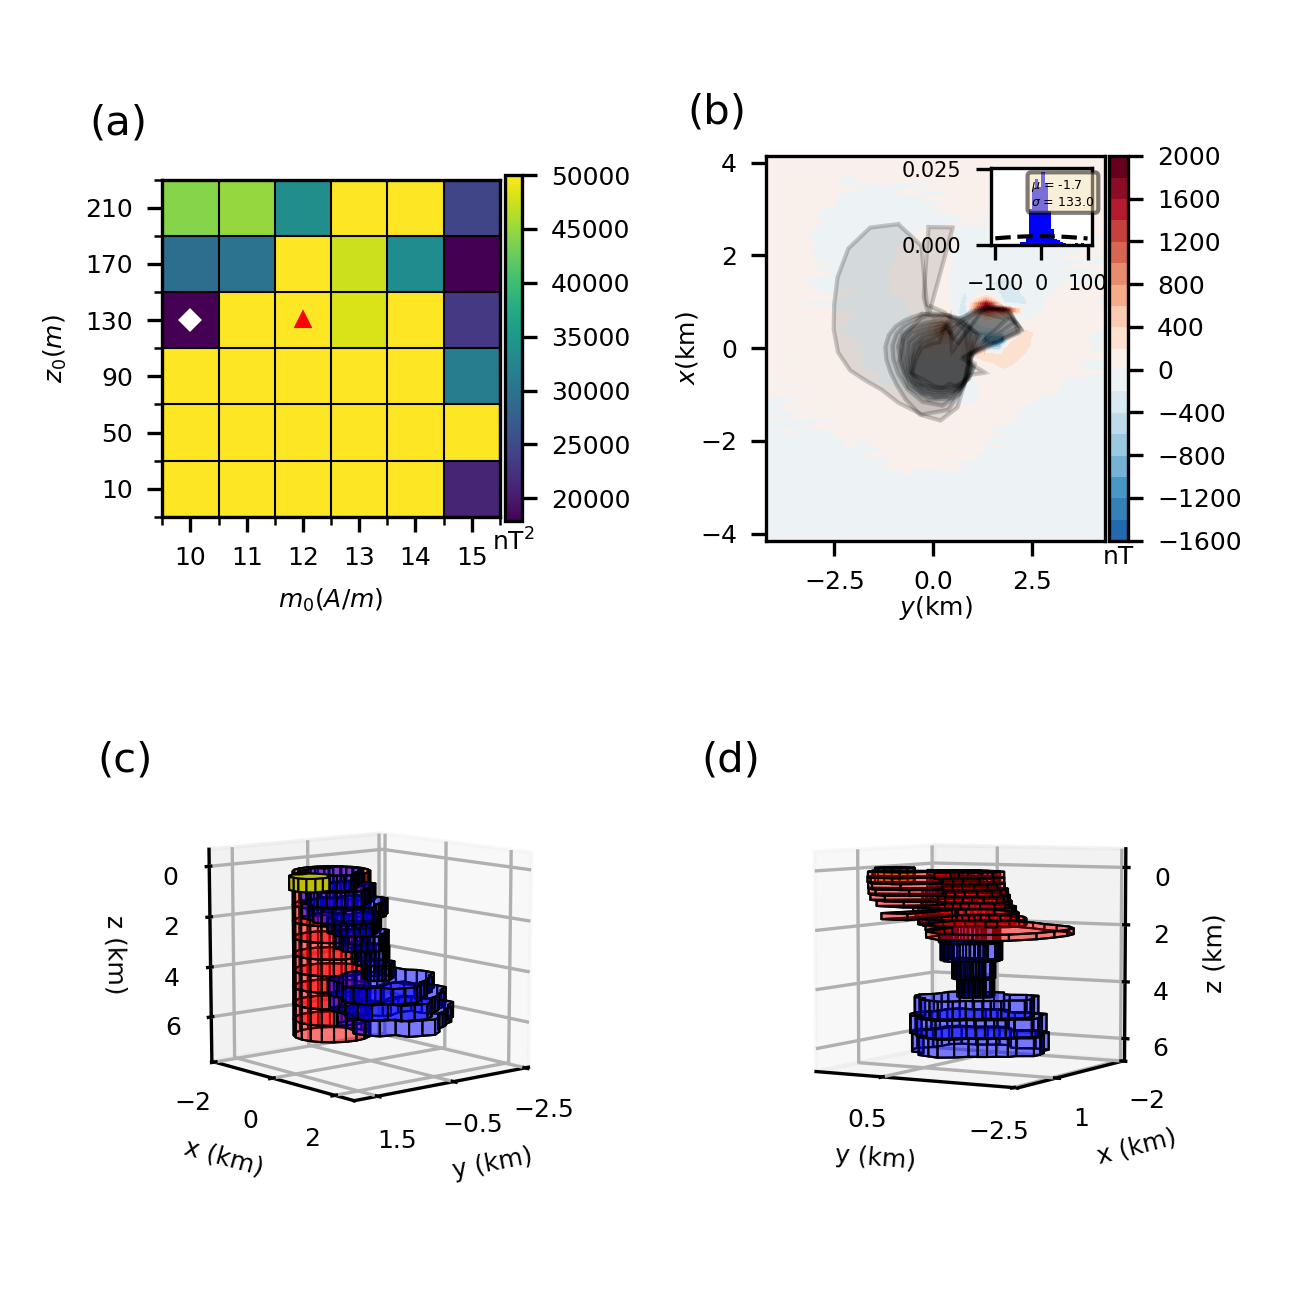
\includegraphics[width=\textwidth]{thick-l2-solution.png}
	\caption{Soluções L2 obtidas para o modelo da fonte alvo com uma fonte não-alvo grande. 
	(a) Mapa discreto da função objetivo produzida pelos modelos da malha de varredura para valores de profundidade do topo $z_{0}$ e intensidade de magnetização total $m_{0}$. 
	Os valores verdadeiros de $m_{0}$ e $z_{0})$ e aqueles que definem a melhor solução L2 são representados pelo triângulo vermelho e pelo losango branco, respectivamente.
	(b) Resíduos entre os dados contaminados com ruído (Figura \ref{fig:target_model}a) 
	e os dados preditos (não mostrados) produzidos pela melhor solução L2 (prismas vermelhos no painel d). 
	O histograma dos resíduos inserido em (b) mostra a curva Gaussiana ajustada (linha tracejada).
	Os polígonos cinzas representam as projeções horizontais de todos os prismas que compõe a melhor solução. 
	(c) e (d) Visualização em perspectiva da aproximação inicial (prismas vermelhos) e 
	a melhor solução (prismas vermelhos), respectivamente. Os prismas azuis são o modelo da fonte alvo. 
	}
	\label{fig:thick_l2_result}
\end{figure}
\pagebreak
\begin{figure}[!htb]
	\centering
	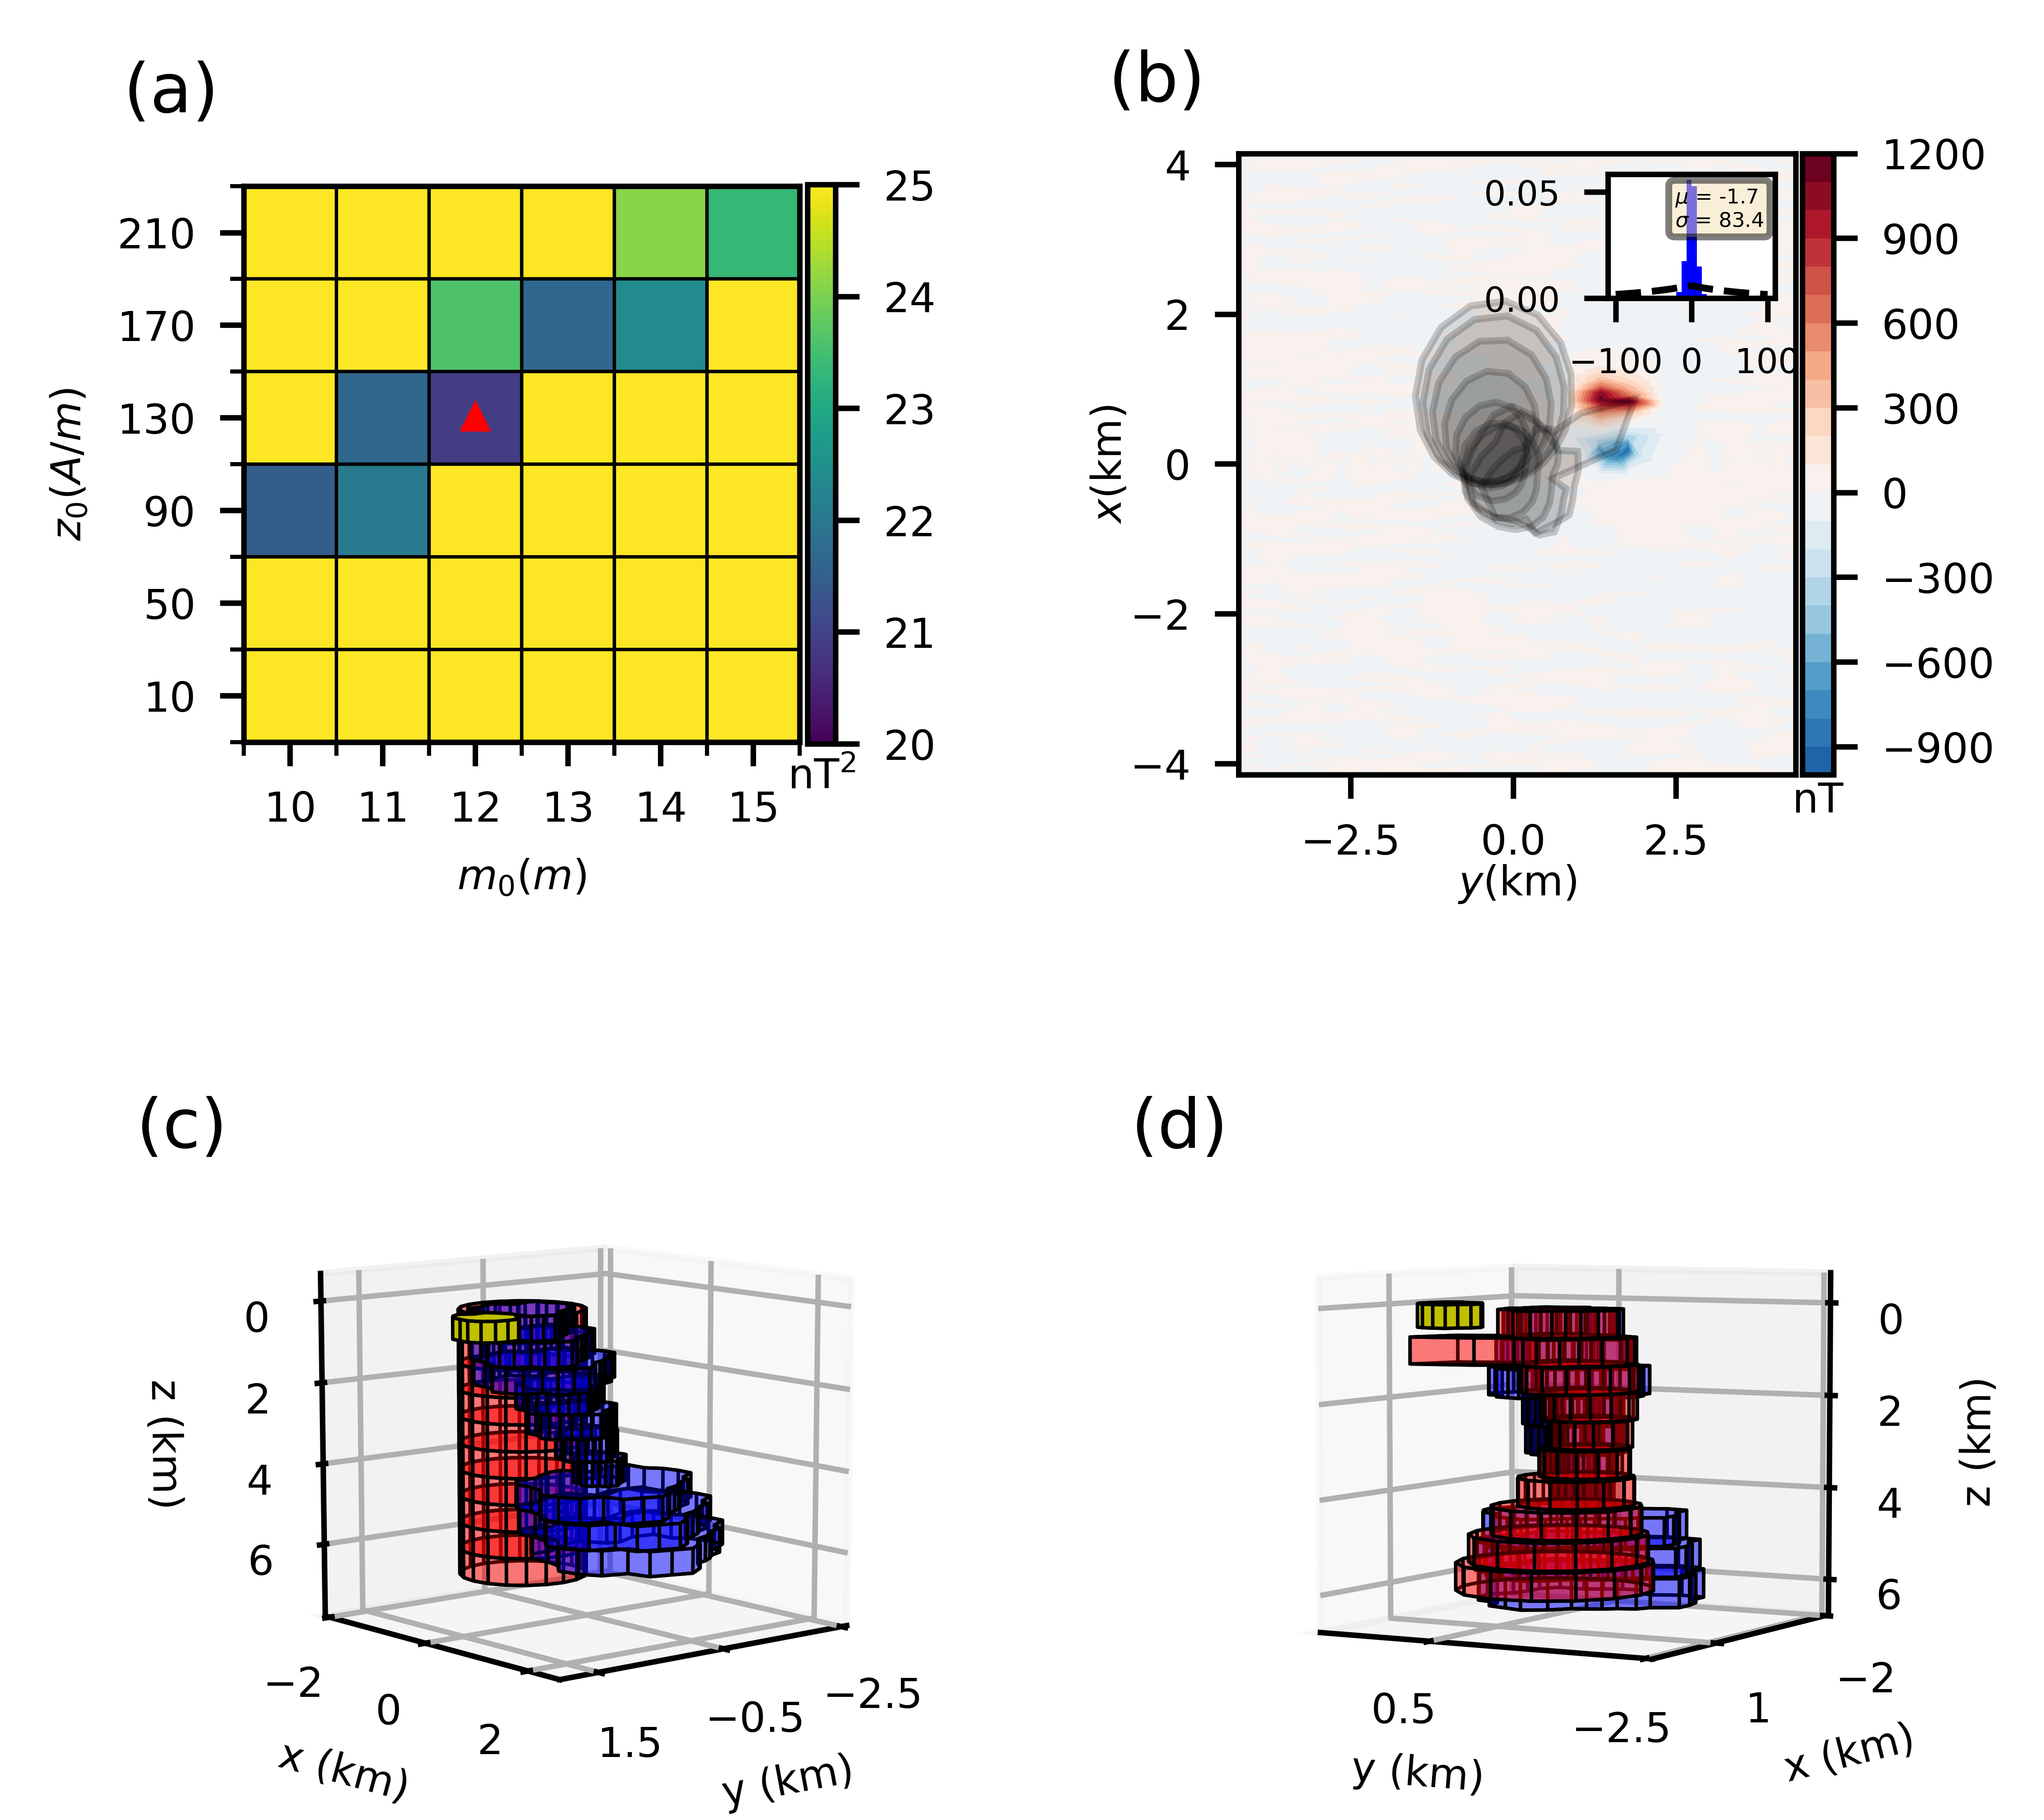
\includegraphics[width=\textwidth]{thick-l1-solution.png}
	\caption{Soluções L1 obtidas para o modelo da fonte alvo com uma fonte não-alvo grande. 
		(a) Mapa discreto da função objetivo produzida pelos modelos da malha de varredura para valores de profundidade do topo $z_{0}$ e intensidade de magnetização total $m_{0}$. 
		Ambos valores verdadeiros de $m_{0}$ e $z_{0})$ e aqueles que definem a melhor solução L1 são representados pelo triângulo vermelho.
		(b) Resíduos entre os dados contaminados com ruído (Figura \ref{fig:target_model}a) 
		e os dados preditos (não mostrados) produzidos pela melhor solução L1 (prismas vermelhos no painel d). 
		O histograma dos resíduos inserido em (b) mostra a curva Gaussiana ajustada (linha tracejada).
		Os polígonos cinzas representam as projeções horizontais de todos os prismas que compõe a melhor solução. 
		(c) e (d) Visualização em perspectiva da aproximação inicial (prismas vermelhos) e 
		a melhor solução (prismas vermelhos), respectivamente. Os prismas azuis são o modelo da fonte alvo. 
	}
	\label{fig:thick_l1_result}
\end{figure}
\pagebreak